\documentclass[twoside]{book}

% Packages required by doxygen
\usepackage{calc}
\usepackage{doxygen}
\usepackage{graphicx}
\usepackage[utf8]{inputenc}
\usepackage{makeidx}
\usepackage{multicol}
\usepackage{multirow}
\usepackage{textcomp}
\usepackage[table]{xcolor}

% Font selection
\usepackage[T1]{fontenc}
\usepackage{mathptmx}
\usepackage[scaled=.90]{helvet}
\usepackage{courier}
\usepackage{amssymb}
\usepackage{sectsty}
\renewcommand{\familydefault}{\sfdefault}
\allsectionsfont{%
  \fontseries{bc}\selectfont%
  \color{darkgray}%
}
\renewcommand{\DoxyLabelFont}{%
  \fontseries{bc}\selectfont%
  \color{darkgray}%
}

% Page & text layout
\usepackage{geometry}
\geometry{%
  a4paper,%
  top=2.5cm,%
  bottom=2.5cm,%
  left=2.5cm,%
  right=2.5cm%
}
\tolerance=750
\hfuzz=15pt
\hbadness=750
\setlength{\emergencystretch}{15pt}
\setlength{\parindent}{0cm}
\setlength{\parskip}{0.2cm}
\makeatletter
\renewcommand{\paragraph}{%
  \@startsection{paragraph}{4}{0ex}{-1.0ex}{1.0ex}{%
    \normalfont\normalsize\bfseries\SS@parafont%
  }%
}
\renewcommand{\subparagraph}{%
  \@startsection{subparagraph}{5}{0ex}{-1.0ex}{1.0ex}{%
    \normalfont\normalsize\bfseries\SS@subparafont%
  }%
}
\makeatother

% Headers & footers
\usepackage{fancyhdr}
\pagestyle{fancyplain}
\fancyhead[LE]{\fancyplain{}{\bfseries\thepage}}
\fancyhead[CE]{\fancyplain{}{}}
\fancyhead[RE]{\fancyplain{}{\bfseries\leftmark}}
\fancyhead[LO]{\fancyplain{}{\bfseries\rightmark}}
\fancyhead[CO]{\fancyplain{}{}}
\fancyhead[RO]{\fancyplain{}{\bfseries\thepage}}
\fancyfoot[LE]{\fancyplain{}{}}
\fancyfoot[CE]{\fancyplain{}{}}
\fancyfoot[RE]{\fancyplain{}{\bfseries\scriptsize Generated on Sun Jun 15 2014 14\-:59\-:46 for U\-T\-Profiler by Doxygen }}
\fancyfoot[LO]{\fancyplain{}{\bfseries\scriptsize Generated on Sun Jun 15 2014 14\-:59\-:46 for U\-T\-Profiler by Doxygen }}
\fancyfoot[CO]{\fancyplain{}{}}
\fancyfoot[RO]{\fancyplain{}{}}
\renewcommand{\footrulewidth}{0.4pt}
\renewcommand{\chaptermark}[1]{%
  \markboth{#1}{}%
}
\renewcommand{\sectionmark}[1]{%
  \markright{\thesection\ #1}%
}

% Indices & bibliography
\usepackage{natbib}
\usepackage[titles]{tocloft}
\setcounter{tocdepth}{3}
\setcounter{secnumdepth}{5}
\makeindex

% Hyperlinks (required, but should be loaded last)
\usepackage{ifpdf}
\ifpdf
  \usepackage[pdftex,pagebackref=true]{hyperref}
\else
  \usepackage[ps2pdf,pagebackref=true]{hyperref}
\fi
\hypersetup{%
  colorlinks=true,%
  linkcolor=blue,%
  citecolor=blue,%
  unicode%
}

% Custom commands
\newcommand{\clearemptydoublepage}{%
  \newpage{\pagestyle{empty}\cleardoublepage}%
}


%===== C O N T E N T S =====

\begin{document}

% Titlepage & ToC
\hypersetup{pageanchor=false}
\pagenumbering{roman}
\begin{titlepage}
\vspace*{7cm}
\begin{center}%
{\Large U\-T\-Profiler \\[1ex]\large 0.\-1 }\\
\vspace*{1cm}
{\large Generated by Doxygen 1.8.6}\\
\vspace*{0.5cm}
{\small Sun Jun 15 2014 14:59:46}\\
\end{center}
\end{titlepage}
\clearemptydoublepage
\tableofcontents
\clearemptydoublepage
\pagenumbering{arabic}
\hypersetup{pageanchor=true}

%--- Begin generated contents ---
\chapter{U\-T\-Profiler}
\label{md__home_timothee__documents__l_o21__u_t_profiler__r_e_a_d_m_e}
\hypertarget{md__home_timothee__documents__l_o21__u_t_profiler__r_e_a_d_m_e}{}
Module de Gestion des U\-Vs de l'U\-T\-C 
\chapter{Hierarchical Index}
\section{Class Hierarchy}
This inheritance list is sorted roughly, but not completely, alphabetically\-:\begin{DoxyCompactList}
\item \contentsline{section}{Dossier}{\pageref{class_dossier}}{}
\item \contentsline{section}{Formation}{\pageref{class_formation}}{}
\item \contentsline{section}{Formation\-Exterieure}{\pageref{class_formation_exterieure}}{}
\item \contentsline{section}{Inscription}{\pageref{class_inscription}}{}
\item \contentsline{section}{Interface\-S\-Q\-L}{\pageref{class_interface_s_q_l}}{}
\item \contentsline{section}{qt\-\_\-meta\-\_\-stringdata\-\_\-\-Associer\-Filiere\-Window\-\_\-t}{\pageref{structqt__meta__stringdata___associer_filiere_window__t}}{}
\item \contentsline{section}{qt\-\_\-meta\-\_\-stringdata\-\_\-\-Associer\-U\-V\-Window\-\_\-t}{\pageref{structqt__meta__stringdata___associer_u_v_window__t}}{}
\item \contentsline{section}{qt\-\_\-meta\-\_\-stringdata\-\_\-\-Completion\-Profil\-Window\-\_\-t}{\pageref{structqt__meta__stringdata___completion_profil_window__t}}{}
\item \contentsline{section}{qt\-\_\-meta\-\_\-stringdata\-\_\-\-Dossier\-Window\-\_\-t}{\pageref{structqt__meta__stringdata___dossier_window__t}}{}
\item \contentsline{section}{qt\-\_\-meta\-\_\-stringdata\-\_\-\-Formation\-Ext\-Window\-\_\-t}{\pageref{structqt__meta__stringdata___formation_ext_window__t}}{}
\item \contentsline{section}{qt\-\_\-meta\-\_\-stringdata\-\_\-\-Formation\-Window\-\_\-t}{\pageref{structqt__meta__stringdata___formation_window__t}}{}
\item \contentsline{section}{qt\-\_\-meta\-\_\-stringdata\-\_\-\-Home\-Window\-\_\-t}{\pageref{structqt__meta__stringdata___home_window__t}}{}
\item \contentsline{section}{qt\-\_\-meta\-\_\-stringdata\-\_\-\-New\-Formation\-Window\-\_\-t}{\pageref{structqt__meta__stringdata___new_formation_window__t}}{}
\item \contentsline{section}{qt\-\_\-meta\-\_\-stringdata\-\_\-\-New\-U\-V\-Window\-\_\-t}{\pageref{structqt__meta__stringdata___new_u_v_window__t}}{}
\item \contentsline{section}{qt\-\_\-meta\-\_\-stringdata\-\_\-\-Retrouver\-Completion\-Window\-\_\-t}{\pageref{structqt__meta__stringdata___retrouver_completion_window__t}}{}
\item \contentsline{section}{qt\-\_\-meta\-\_\-stringdata\-\_\-\-Search\-Dossier\-Window\-\_\-t}{\pageref{structqt__meta__stringdata___search_dossier_window__t}}{}
\item \contentsline{section}{qt\-\_\-meta\-\_\-stringdata\-\_\-\-Semestre\-Window\-\_\-t}{\pageref{structqt__meta__stringdata___semestre_window__t}}{}
\item \contentsline{section}{qt\-\_\-meta\-\_\-stringdata\-\_\-\-U\-V\-Window\-\_\-t}{\pageref{structqt__meta__stringdata___u_v_window__t}}{}
\item Q\-Widget\begin{DoxyCompactList}
\item \contentsline{section}{Associer\-Filiere\-Window}{\pageref{class_associer_filiere_window}}{}
\item \contentsline{section}{Associer\-U\-V\-Window}{\pageref{class_associer_u_v_window}}{}
\item \contentsline{section}{Completion\-Profil\-Window}{\pageref{class_completion_profil_window}}{}
\item \contentsline{section}{Dossier\-Window}{\pageref{class_dossier_window}}{}
\item \contentsline{section}{Formation\-Ext\-Window}{\pageref{class_formation_ext_window}}{}
\item \contentsline{section}{Formation\-Window}{\pageref{class_formation_window}}{}
\item \contentsline{section}{Home\-Window}{\pageref{class_home_window}}{}
\item \contentsline{section}{New\-Formation\-Window}{\pageref{class_new_formation_window}}{}
\item \contentsline{section}{New\-U\-V\-Window}{\pageref{class_new_u_v_window}}{}
\item \contentsline{section}{Retrouver\-Completion\-Window}{\pageref{class_retrouver_completion_window}}{}
\item \contentsline{section}{Search\-Dossier\-Window}{\pageref{class_search_dossier_window}}{}
\item \contentsline{section}{Semestre\-Window}{\pageref{class_semestre_window}}{}
\item \contentsline{section}{U\-V\-Window}{\pageref{class_u_v_window}}{}
\end{DoxyCompactList}
\item \contentsline{section}{Semestre}{\pageref{class_semestre}}{}
\item \contentsline{section}{U\-T\-Profiler\-Exception}{\pageref{class_u_t_profiler_exception}}{}
\item \contentsline{section}{U\-V}{\pageref{class_u_v}}{}
\end{DoxyCompactList}

\chapter{Class Index}
\section{Class List}
Here are the classes, structs, unions and interfaces with brief descriptions\-:\begin{DoxyCompactList}
\item\contentsline{section}{\hyperlink{class_associer_filiere_window}{Associer\-Filiere\-Window} \\*Classe de la fenêtre pour associer une filière à une branche }{\pageref{class_associer_filiere_window}}{}
\item\contentsline{section}{\hyperlink{class_associer_u_v_window}{Associer\-U\-V\-Window} \\*Classe de la fenêtre pour associer une uv à une formation }{\pageref{class_associer_u_v_window}}{}
\item\contentsline{section}{\hyperlink{class_completion_profil_window}{Completion\-Profil\-Window} }{\pageref{class_completion_profil_window}}{}
\item\contentsline{section}{\hyperlink{class_dossier}{Dossier} \\*Classe représentant un dossier }{\pageref{class_dossier}}{}
\item\contentsline{section}{\hyperlink{class_dossier_window}{Dossier\-Window} \\*Classe pour la fenêtre qui permet de consulter, modifier, ajouter, supprimer un dossier }{\pageref{class_dossier_window}}{}
\item\contentsline{section}{\hyperlink{class_formation}{Formation} \\*Classe représentant une formation }{\pageref{class_formation}}{}
\item\contentsline{section}{\hyperlink{class_formation_exterieure}{Formation\-Exterieure} \\*Classe permettant de décrire une formation extérieure à l'U\-T\-C mais rapportant un certain nombre de crédits par équivalence }{\pageref{class_formation_exterieure}}{}
\item\contentsline{section}{\hyperlink{class_formation_ext_window}{Formation\-Ext\-Window} \\*Classe qui permet d'ajouter une formation extérieure à un login existant }{\pageref{class_formation_ext_window}}{}
\item\contentsline{section}{\hyperlink{class_formation_window}{Formation\-Window} \\*Classe de la fenêtre pour la gestion des formations }{\pageref{class_formation_window}}{}
\item\contentsline{section}{\hyperlink{class_home_window}{Home\-Window} \\*Classe de la fenêtre d'accueil de U\-T\-Profiler }{\pageref{class_home_window}}{}
\item\contentsline{section}{\hyperlink{class_inscription}{Inscription} \\*Classe permettant de décrire l'inscription d'un étudiant à une \hyperlink{class_u_v}{U\-V} de l'U\-T\-C }{\pageref{class_inscription}}{}
\item\contentsline{section}{\hyperlink{class_interface_s_q_l}{Interface\-S\-Q\-L} \\*Classe permettant la communication avec la base de données }{\pageref{class_interface_s_q_l}}{}
\item\contentsline{section}{\hyperlink{class_new_formation_window}{New\-Formation\-Window} \\*Classe qui permet d'ajouter une nouvelle formation }{\pageref{class_new_formation_window}}{}
\item\contentsline{section}{\hyperlink{class_new_u_v_window}{New\-U\-V\-Window} }{\pageref{class_new_u_v_window}}{}
\item\contentsline{section}{\hyperlink{structqt__meta__stringdata___associer_filiere_window__t}{qt\-\_\-meta\-\_\-stringdata\-\_\-\-Associer\-Filiere\-Window\-\_\-t} }{\pageref{structqt__meta__stringdata___associer_filiere_window__t}}{}
\item\contentsline{section}{\hyperlink{structqt__meta__stringdata___associer_u_v_window__t}{qt\-\_\-meta\-\_\-stringdata\-\_\-\-Associer\-U\-V\-Window\-\_\-t} }{\pageref{structqt__meta__stringdata___associer_u_v_window__t}}{}
\item\contentsline{section}{\hyperlink{structqt__meta__stringdata___completion_profil_window__t}{qt\-\_\-meta\-\_\-stringdata\-\_\-\-Completion\-Profil\-Window\-\_\-t} }{\pageref{structqt__meta__stringdata___completion_profil_window__t}}{}
\item\contentsline{section}{\hyperlink{structqt__meta__stringdata___dossier_window__t}{qt\-\_\-meta\-\_\-stringdata\-\_\-\-Dossier\-Window\-\_\-t} }{\pageref{structqt__meta__stringdata___dossier_window__t}}{}
\item\contentsline{section}{\hyperlink{structqt__meta__stringdata___formation_ext_window__t}{qt\-\_\-meta\-\_\-stringdata\-\_\-\-Formation\-Ext\-Window\-\_\-t} }{\pageref{structqt__meta__stringdata___formation_ext_window__t}}{}
\item\contentsline{section}{\hyperlink{structqt__meta__stringdata___formation_window__t}{qt\-\_\-meta\-\_\-stringdata\-\_\-\-Formation\-Window\-\_\-t} }{\pageref{structqt__meta__stringdata___formation_window__t}}{}
\item\contentsline{section}{\hyperlink{structqt__meta__stringdata___home_window__t}{qt\-\_\-meta\-\_\-stringdata\-\_\-\-Home\-Window\-\_\-t} }{\pageref{structqt__meta__stringdata___home_window__t}}{}
\item\contentsline{section}{\hyperlink{structqt__meta__stringdata___new_formation_window__t}{qt\-\_\-meta\-\_\-stringdata\-\_\-\-New\-Formation\-Window\-\_\-t} }{\pageref{structqt__meta__stringdata___new_formation_window__t}}{}
\item\contentsline{section}{\hyperlink{structqt__meta__stringdata___new_u_v_window__t}{qt\-\_\-meta\-\_\-stringdata\-\_\-\-New\-U\-V\-Window\-\_\-t} }{\pageref{structqt__meta__stringdata___new_u_v_window__t}}{}
\item\contentsline{section}{\hyperlink{structqt__meta__stringdata___retrouver_completion_window__t}{qt\-\_\-meta\-\_\-stringdata\-\_\-\-Retrouver\-Completion\-Window\-\_\-t} }{\pageref{structqt__meta__stringdata___retrouver_completion_window__t}}{}
\item\contentsline{section}{\hyperlink{structqt__meta__stringdata___search_dossier_window__t}{qt\-\_\-meta\-\_\-stringdata\-\_\-\-Search\-Dossier\-Window\-\_\-t} }{\pageref{structqt__meta__stringdata___search_dossier_window__t}}{}
\item\contentsline{section}{\hyperlink{structqt__meta__stringdata___semestre_window__t}{qt\-\_\-meta\-\_\-stringdata\-\_\-\-Semestre\-Window\-\_\-t} }{\pageref{structqt__meta__stringdata___semestre_window__t}}{}
\item\contentsline{section}{\hyperlink{structqt__meta__stringdata___u_v_window__t}{qt\-\_\-meta\-\_\-stringdata\-\_\-\-U\-V\-Window\-\_\-t} }{\pageref{structqt__meta__stringdata___u_v_window__t}}{}
\item\contentsline{section}{\hyperlink{class_retrouver_completion_window}{Retrouver\-Completion\-Window} }{\pageref{class_retrouver_completion_window}}{}
\item\contentsline{section}{\hyperlink{class_search_dossier_window}{Search\-Dossier\-Window} }{\pageref{class_search_dossier_window}}{}
\item\contentsline{section}{\hyperlink{class_semestre}{Semestre} \\*Classe permettant de décrire un semestre d'un étudiant de l'U\-T\-C }{\pageref{class_semestre}}{}
\item\contentsline{section}{\hyperlink{class_semestre_window}{Semestre\-Window} \\*Classe qui permet d'ajouter un semestre/une inscription à un uv, à un login existant }{\pageref{class_semestre_window}}{}
\item\contentsline{section}{\hyperlink{class_u_t_profiler_exception}{U\-T\-Profiler\-Exception} \\*Classe permettant de gérer l'ensemble des exceptions de l'application }{\pageref{class_u_t_profiler_exception}}{}
\item\contentsline{section}{\hyperlink{class_u_v}{U\-V} \\*Classe permettant de décrire une des U\-Vs de l'U\-T\-C }{\pageref{class_u_v}}{}
\item\contentsline{section}{\hyperlink{class_u_v_window}{U\-V\-Window} }{\pageref{class_u_v_window}}{}
\end{DoxyCompactList}

\chapter{File Index}
\section{File List}
Here is a list of all documented files with brief descriptions\-:\begin{DoxyCompactList}
\item\contentsline{section}{/home/timothee/\-Documents/\-L\-O21/\-U\-T\-Profiler/build-\/\-U\-T\-Profiler-\/\-Desktop-\/\-Debug/{\bfseries moc\-\_\-\-U\-T\-Profiler.\-cpp} }{\pageref{moc___u_t_profiler_8cpp}}{}
\item\contentsline{section}{{\bfseries Completion\-Profil\-Window.\-cpp} }{\pageref{_completion_profil_window_8cpp}}{}
\item\contentsline{section}{\hyperlink{_dossier_window_8cpp}{Dossier\-Window.\-cpp} \\*Fenêtre de gestion des dossiers }{\pageref{_dossier_window_8cpp}}{}
\item\contentsline{section}{\hyperlink{_formation_window_8cpp}{Formation\-Window.\-cpp} \\*Fenêtre de gestion des formations }{\pageref{_formation_window_8cpp}}{}
\item\contentsline{section}{\hyperlink{_home_window_8cpp}{Home\-Window.\-cpp} \\*Fenêtre d'accueil de U\-T\-Profiler }{\pageref{_home_window_8cpp}}{}
\item\contentsline{section}{\hyperlink{_interface_s_q_l_8cpp}{Interface\-S\-Q\-L.\-cpp} \\*Fichier source où sont implémentées les méthodes de la classe \hyperlink{class_interface_s_q_l}{Interface\-S\-Q\-L} }{\pageref{_interface_s_q_l_8cpp}}{}
\item\contentsline{section}{{\bfseries main.\-cpp} }{\pageref{main_8cpp}}{}
\item\contentsline{section}{{\bfseries U\-T\-Profiler.\-cpp} }{\pageref{_u_t_profiler_8cpp}}{}
\item\contentsline{section}{\hyperlink{_u_t_profiler_8h}{U\-T\-Profiler.\-h} \\*Ce header recense les déclarations de toutes nos classes }{\pageref{_u_t_profiler_8h}}{}
\item\contentsline{section}{{\bfseries U\-V\-Window.\-cpp} }{\pageref{_u_v_window_8cpp}}{}
\end{DoxyCompactList}

\chapter{Class Documentation}
\hypertarget{class_associer_filiere_window}{\section{Associer\-Filiere\-Window Class Reference}
\label{class_associer_filiere_window}\index{Associer\-Filiere\-Window@{Associer\-Filiere\-Window}}
}


Classe de la fenêtre pour associer une filière à une branche.  




{\ttfamily \#include $<$U\-T\-Profiler.\-h$>$}



Inheritance diagram for Associer\-Filiere\-Window\-:
\nopagebreak
\begin{figure}[H]
\begin{center}
\leavevmode
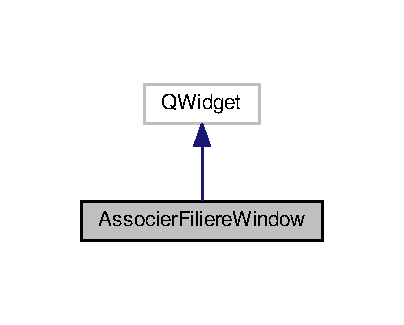
\includegraphics[width=194pt]{class_associer_filiere_window__inherit__graph}
\end{center}
\end{figure}


Collaboration diagram for Associer\-Filiere\-Window\-:
\nopagebreak
\begin{figure}[H]
\begin{center}
\leavevmode
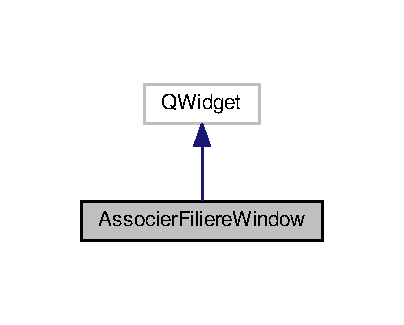
\includegraphics[width=194pt]{class_associer_filiere_window__coll__graph}
\end{center}
\end{figure}
\subsection*{Public Slots}
\begin{DoxyCompactItemize}
\item 
\hypertarget{class_associer_filiere_window_ae5b2e89b675c54c9a797368d6b4f7b8c}{void \hyperlink{class_associer_filiere_window_ae5b2e89b675c54c9a797368d6b4f7b8c}{ajouter} ()}\label{class_associer_filiere_window_ae5b2e89b675c54c9a797368d6b4f7b8c}

\begin{DoxyCompactList}\small\item\em Association d'une filière à une branche. \end{DoxyCompactList}\end{DoxyCompactItemize}
\subsection*{Public Member Functions}
\begin{DoxyCompactItemize}
\item 
\hyperlink{class_associer_filiere_window_ae970aceb1a4b9fdfbf2e12ff630478a0}{Associer\-Filiere\-Window} (const Q\-String \&b)
\begin{DoxyCompactList}\small\item\em Constructeur de \hyperlink{class_associer_filiere_window}{Associer\-Filiere\-Window}. \end{DoxyCompactList}\item 
Q\-String \hyperlink{class_associer_filiere_window_aeb96bfea5e2dcc59cc49b47196a2298f}{get\-Branche} () const 
\begin{DoxyCompactList}\small\item\em Accès en lecture à la branche. \end{DoxyCompactList}\end{DoxyCompactItemize}


\subsection{Detailed Description}
Classe de la fenêtre pour associer une filière à une branche. 

Definition at line 1449 of file U\-T\-Profiler.\-h.



\subsection{Constructor \& Destructor Documentation}
\hypertarget{class_associer_filiere_window_ae970aceb1a4b9fdfbf2e12ff630478a0}{\index{Associer\-Filiere\-Window@{Associer\-Filiere\-Window}!Associer\-Filiere\-Window@{Associer\-Filiere\-Window}}
\index{Associer\-Filiere\-Window@{Associer\-Filiere\-Window}!AssocierFiliereWindow@{Associer\-Filiere\-Window}}
\subsubsection[{Associer\-Filiere\-Window}]{\setlength{\rightskip}{0pt plus 5cm}Associer\-Filiere\-Window\-::\-Associer\-Filiere\-Window (
\begin{DoxyParamCaption}
\item[{const Q\-String \&}]{b}
\end{DoxyParamCaption}
)}}\label{class_associer_filiere_window_ae970aceb1a4b9fdfbf2e12ff630478a0}


Constructeur de \hyperlink{class_associer_filiere_window}{Associer\-Filiere\-Window}. 


\begin{DoxyParams}{Parameters}
{\em b} & \-: branche pour laquelle on associe une filière \\
\hline
\end{DoxyParams}


Definition at line 689 of file Formation\-Window.\-cpp.



\subsection{Member Function Documentation}
\hypertarget{class_associer_filiere_window_aeb96bfea5e2dcc59cc49b47196a2298f}{\index{Associer\-Filiere\-Window@{Associer\-Filiere\-Window}!get\-Branche@{get\-Branche}}
\index{get\-Branche@{get\-Branche}!AssocierFiliereWindow@{Associer\-Filiere\-Window}}
\subsubsection[{get\-Branche}]{\setlength{\rightskip}{0pt plus 5cm}Q\-String Associer\-Filiere\-Window\-::get\-Branche (
\begin{DoxyParamCaption}
{}
\end{DoxyParamCaption}
) const\hspace{0.3cm}{\ttfamily [inline]}}}\label{class_associer_filiere_window_aeb96bfea5e2dcc59cc49b47196a2298f}


Accès en lecture à la branche. 

\begin{DoxyReturn}{Returns}
l'attribut branche 
\end{DoxyReturn}


Definition at line 1468 of file U\-T\-Profiler.\-h.



The documentation for this class was generated from the following files\-:\begin{DoxyCompactItemize}
\item 
\hyperlink{_u_t_profiler_8h}{U\-T\-Profiler.\-h}\item 
\hyperlink{_formation_window_8cpp}{Formation\-Window.\-cpp}\end{DoxyCompactItemize}

\hypertarget{class_associer_u_v_window}{\section{Associer\-U\-V\-Window Class Reference}
\label{class_associer_u_v_window}\index{Associer\-U\-V\-Window@{Associer\-U\-V\-Window}}
}


Classe de la fenêtre pour associer une uv à une formation.  




{\ttfamily \#include $<$U\-T\-Profiler.\-h$>$}



Inheritance diagram for Associer\-U\-V\-Window\-:
\nopagebreak
\begin{figure}[H]
\begin{center}
\leavevmode
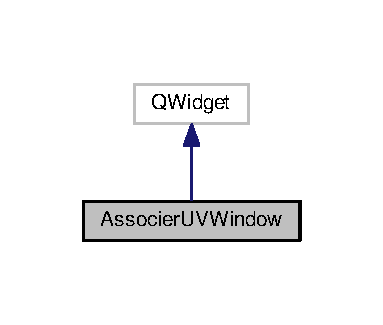
\includegraphics[width=184pt]{class_associer_u_v_window__inherit__graph}
\end{center}
\end{figure}


Collaboration diagram for Associer\-U\-V\-Window\-:
\nopagebreak
\begin{figure}[H]
\begin{center}
\leavevmode
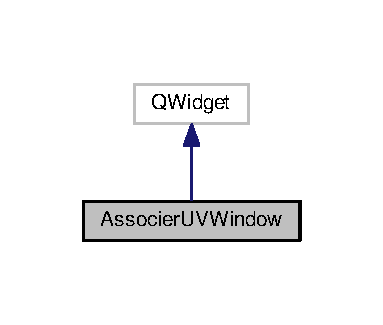
\includegraphics[width=184pt]{class_associer_u_v_window__coll__graph}
\end{center}
\end{figure}
\subsection*{Public Slots}
\begin{DoxyCompactItemize}
\item 
\hypertarget{class_associer_u_v_window_a0a317e5f5fc2a182d181d642a7cd8d6d}{void \hyperlink{class_associer_u_v_window_a0a317e5f5fc2a182d181d642a7cd8d6d}{ajouter} ()}\label{class_associer_u_v_window_a0a317e5f5fc2a182d181d642a7cd8d6d}

\begin{DoxyCompactList}\small\item\em Association d'une uv à une formation. \end{DoxyCompactList}\end{DoxyCompactItemize}
\subsection*{Public Member Functions}
\begin{DoxyCompactItemize}
\item 
\hyperlink{class_associer_u_v_window_a7576d2e8d391e83db75a05885b39af9e}{Associer\-U\-V\-Window} (const Q\-String \&f)
\begin{DoxyCompactList}\small\item\em Constructeur de \hyperlink{class_associer_u_v_window}{Associer\-U\-V\-Window}. \end{DoxyCompactList}\item 
Q\-String \hyperlink{class_associer_u_v_window_a457cac65cea8a0ef928207f5061aaeb2}{get\-Formation} () const 
\begin{DoxyCompactList}\small\item\em Accès en lecture à la formation. \end{DoxyCompactList}\end{DoxyCompactItemize}


\subsection{Detailed Description}
Classe de la fenêtre pour associer une uv à une formation. 

Definition at line 1421 of file U\-T\-Profiler.\-h.



\subsection{Constructor \& Destructor Documentation}
\hypertarget{class_associer_u_v_window_a7576d2e8d391e83db75a05885b39af9e}{\index{Associer\-U\-V\-Window@{Associer\-U\-V\-Window}!Associer\-U\-V\-Window@{Associer\-U\-V\-Window}}
\index{Associer\-U\-V\-Window@{Associer\-U\-V\-Window}!AssocierUVWindow@{Associer\-U\-V\-Window}}
\subsubsection[{Associer\-U\-V\-Window}]{\setlength{\rightskip}{0pt plus 5cm}Associer\-U\-V\-Window\-::\-Associer\-U\-V\-Window (
\begin{DoxyParamCaption}
\item[{const Q\-String \&}]{f}
\end{DoxyParamCaption}
)}}\label{class_associer_u_v_window_a7576d2e8d391e83db75a05885b39af9e}


Constructeur de \hyperlink{class_associer_u_v_window}{Associer\-U\-V\-Window}. 


\begin{DoxyParams}{Parameters}
{\em f} & \-: formation pour laquelle on associe une uv \\
\hline
\end{DoxyParams}


Definition at line 608 of file Formation\-Window.\-cpp.



\subsection{Member Function Documentation}
\hypertarget{class_associer_u_v_window_a457cac65cea8a0ef928207f5061aaeb2}{\index{Associer\-U\-V\-Window@{Associer\-U\-V\-Window}!get\-Formation@{get\-Formation}}
\index{get\-Formation@{get\-Formation}!AssocierUVWindow@{Associer\-U\-V\-Window}}
\subsubsection[{get\-Formation}]{\setlength{\rightskip}{0pt plus 5cm}Q\-String Associer\-U\-V\-Window\-::get\-Formation (
\begin{DoxyParamCaption}
{}
\end{DoxyParamCaption}
) const\hspace{0.3cm}{\ttfamily [inline]}}}\label{class_associer_u_v_window_a457cac65cea8a0ef928207f5061aaeb2}


Accès en lecture à la formation. 

\begin{DoxyReturn}{Returns}
l'attribut formation 
\end{DoxyReturn}


Definition at line 1440 of file U\-T\-Profiler.\-h.



The documentation for this class was generated from the following files\-:\begin{DoxyCompactItemize}
\item 
\hyperlink{_u_t_profiler_8h}{U\-T\-Profiler.\-h}\item 
\hyperlink{_formation_window_8cpp}{Formation\-Window.\-cpp}\end{DoxyCompactItemize}

\hypertarget{class_completion_profil_window}{\section{Completion\-Profil\-Window Class Reference}
\label{class_completion_profil_window}\index{Completion\-Profil\-Window@{Completion\-Profil\-Window}}
}


Inheritance diagram for Completion\-Profil\-Window\-:
\nopagebreak
\begin{figure}[H]
\begin{center}
\leavevmode
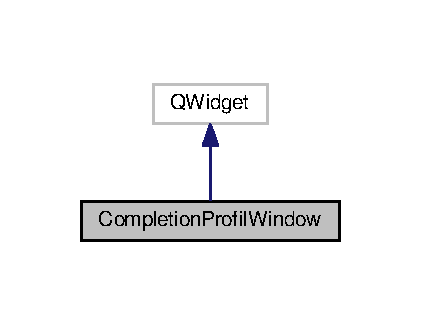
\includegraphics[width=202pt]{class_completion_profil_window__inherit__graph}
\end{center}
\end{figure}


Collaboration diagram for Completion\-Profil\-Window\-:
\nopagebreak
\begin{figure}[H]
\begin{center}
\leavevmode
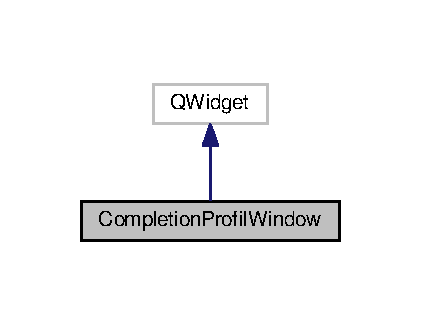
\includegraphics[width=202pt]{class_completion_profil_window__coll__graph}
\end{center}
\end{figure}
\subsection*{Public Slots}
\begin{DoxyCompactItemize}
\item 
\hypertarget{class_completion_profil_window_ac0be1871923bef6992015e5a63d47c3b}{void \hyperlink{class_completion_profil_window_ac0be1871923bef6992015e5a63d47c3b}{rechercher} ()}\label{class_completion_profil_window_ac0be1871923bef6992015e5a63d47c3b}

\begin{DoxyCompactList}\small\item\em Slot ouvrant la fenetre de recherche de dossier. \end{DoxyCompactList}\item 
\hypertarget{class_completion_profil_window_a76e6fa43ca5d053ca5c61a2b5f85d550}{void \hyperlink{class_completion_profil_window_a76e6fa43ca5d053ca5c61a2b5f85d550}{enregistrer} ()}\label{class_completion_profil_window_a76e6fa43ca5d053ca5c61a2b5f85d550}

\begin{DoxyCompactList}\small\item\em Slot permettant d'enregistrer une completion dont toutes les U\-Vs sont confirmées dans la base de données pour qu'elle puisse être reconsultée plus tard. \end{DoxyCompactList}\item 
\hypertarget{class_completion_profil_window_a2d9eafb639de00df21045450fc622ec6}{void \hyperlink{class_completion_profil_window_a2d9eafb639de00df21045450fc622ec6}{confirmer1} ()}\label{class_completion_profil_window_a2d9eafb639de00df21045450fc622ec6}

\begin{DoxyCompactList}\small\item\em Slot permettant de valider une \hyperlink{class_u_v}{U\-V} parmi les suggestions. \end{DoxyCompactList}\item 
\hypertarget{class_completion_profil_window_a279a78595903d7d6be1ff0b175345391}{void \hyperlink{class_completion_profil_window_a279a78595903d7d6be1ff0b175345391}{confirmer2} ()}\label{class_completion_profil_window_a279a78595903d7d6be1ff0b175345391}

\begin{DoxyCompactList}\small\item\em Slot permettant de valider une \hyperlink{class_u_v}{U\-V} parmi les suggestions. \end{DoxyCompactList}\item 
\hypertarget{class_completion_profil_window_a073eb07059b6e57b4318759daf61db44}{void \hyperlink{class_completion_profil_window_a073eb07059b6e57b4318759daf61db44}{confirmer3} ()}\label{class_completion_profil_window_a073eb07059b6e57b4318759daf61db44}

\begin{DoxyCompactList}\small\item\em Slot permettant de valider une \hyperlink{class_u_v}{U\-V} parmi les suggestions. \end{DoxyCompactList}\item 
\hypertarget{class_completion_profil_window_a45c8313e38ff50eda2f2953e04ff22cb}{void \hyperlink{class_completion_profil_window_a45c8313e38ff50eda2f2953e04ff22cb}{confirmer4} ()}\label{class_completion_profil_window_a45c8313e38ff50eda2f2953e04ff22cb}

\begin{DoxyCompactList}\small\item\em Slot permettant de valider une \hyperlink{class_u_v}{U\-V} parmi les suggestions. \end{DoxyCompactList}\item 
\hypertarget{class_completion_profil_window_aebfd868d226674cb60a98cd418e9657e}{void {\bfseries confirmer5} ()}\label{class_completion_profil_window_aebfd868d226674cb60a98cd418e9657e}

\item 
\hypertarget{class_completion_profil_window_a83b5e31dcf228301a0c1ae1bf887c0c7}{void \hyperlink{class_completion_profil_window_a83b5e31dcf228301a0c1ae1bf887c0c7}{confirmer6} ()}\label{class_completion_profil_window_a83b5e31dcf228301a0c1ae1bf887c0c7}

\begin{DoxyCompactList}\small\item\em Slot permettant de valider une \hyperlink{class_u_v}{U\-V} parmi les suggestions. \end{DoxyCompactList}\item 
\hypertarget{class_completion_profil_window_a214d3561805bff336fa67967d22c0b68}{void \hyperlink{class_completion_profil_window_a214d3561805bff336fa67967d22c0b68}{refuser1} ()}\label{class_completion_profil_window_a214d3561805bff336fa67967d22c0b68}

\begin{DoxyCompactList}\small\item\em Slot permettant de refuser une \hyperlink{class_u_v}{U\-V} parmi les suggestions, et de demander à l'algorithme d'en proposer une autre à la place. \end{DoxyCompactList}\item 
\hypertarget{class_completion_profil_window_ac441db2632b8506ad4399f722b5bb159}{void \hyperlink{class_completion_profil_window_ac441db2632b8506ad4399f722b5bb159}{refuser2} ()}\label{class_completion_profil_window_ac441db2632b8506ad4399f722b5bb159}

\begin{DoxyCompactList}\small\item\em Slot permettant de refuser une \hyperlink{class_u_v}{U\-V} parmi les suggestions, et de demander à l'algorithme d'en proposer une autre à la place. \end{DoxyCompactList}\item 
\hypertarget{class_completion_profil_window_ad30b74a40d832022170ec38bf933465a}{void \hyperlink{class_completion_profil_window_ad30b74a40d832022170ec38bf933465a}{refuser3} ()}\label{class_completion_profil_window_ad30b74a40d832022170ec38bf933465a}

\begin{DoxyCompactList}\small\item\em Slot permettant de refuser une \hyperlink{class_u_v}{U\-V} parmi les suggestions, et de demander à l'algorithme d'en proposer une autre à la place. \end{DoxyCompactList}\item 
\hypertarget{class_completion_profil_window_ac9f7cdc86e6a4891898f5b6c34e9e3c1}{void \hyperlink{class_completion_profil_window_ac9f7cdc86e6a4891898f5b6c34e9e3c1}{refuser4} ()}\label{class_completion_profil_window_ac9f7cdc86e6a4891898f5b6c34e9e3c1}

\begin{DoxyCompactList}\small\item\em Slot permettant de refuser une \hyperlink{class_u_v}{U\-V} parmi les suggestions, et de demander à l'algorithme d'en proposer une autre à la place. \end{DoxyCompactList}\item 
\hypertarget{class_completion_profil_window_abeca09ee116c6960e5535ab724d6ad8a}{void \hyperlink{class_completion_profil_window_abeca09ee116c6960e5535ab724d6ad8a}{refuser5} ()}\label{class_completion_profil_window_abeca09ee116c6960e5535ab724d6ad8a}

\begin{DoxyCompactList}\small\item\em Slot permettant de refuser une \hyperlink{class_u_v}{U\-V} parmi les suggestions, et de demander à l'algorithme d'en proposer une autre à la place. \end{DoxyCompactList}\item 
\hypertarget{class_completion_profil_window_ad1dd6d8ba2e161d2cf8bc0deaeddb46b}{void \hyperlink{class_completion_profil_window_ad1dd6d8ba2e161d2cf8bc0deaeddb46b}{refuser6} ()}\label{class_completion_profil_window_ad1dd6d8ba2e161d2cf8bc0deaeddb46b}

\begin{DoxyCompactList}\small\item\em Slot permettant de refuser une \hyperlink{class_u_v}{U\-V} parmi les suggestions, et de demander à l'algorithme d'en proposer une autre à la place. \end{DoxyCompactList}\end{DoxyCompactItemize}
\subsection*{Public Member Functions}
\begin{DoxyCompactItemize}
\item 
\hypertarget{class_completion_profil_window_a41997a68d2025526bb8b7e44a2d0fd95}{\hyperlink{class_completion_profil_window_a41997a68d2025526bb8b7e44a2d0fd95}{Completion\-Profil\-Window} ()}\label{class_completion_profil_window_a41997a68d2025526bb8b7e44a2d0fd95}

\begin{DoxyCompactList}\small\item\em Constructeur Ce constructeur initialise toutes les fonctions de l'Interface Graphique de cette fenêtre \-: créer et organiser les objets graphiques, et les connecter avec les bons slots. \end{DoxyCompactList}\item 
void \hyperlink{class_completion_profil_window_a217a870ed07c3b7157422195e21e1422}{Completion\-Profil} (\hyperlink{class_dossier}{Dossier} $\ast$dossier, Q\-String $\ast$$\ast$souhaits, Q\-String $\ast$$\ast$rejets)
\begin{DoxyCompactList}\small\item\em Algorithme de Completion de Profil. \end{DoxyCompactList}\item 
\hypertarget{class_completion_profil_window_a895aed548c69ea5c5953165ef4b11c3b}{void {\bfseries associercompletion} (\hyperlink{class_u_v}{U\-V} $\ast$$\ast$uvs)}\label{class_completion_profil_window_a895aed548c69ea5c5953165ef4b11c3b}

\end{DoxyCompactItemize}
\subsection*{Friends}
\begin{DoxyCompactItemize}
\item 
\hypertarget{class_completion_profil_window_a89f0e38a39f054c26a0ab852f8a79b18}{class {\bfseries Home\-Window}}\label{class_completion_profil_window_a89f0e38a39f054c26a0ab852f8a79b18}

\end{DoxyCompactItemize}


\subsection{Detailed Description}


Definition at line 1328 of file U\-T\-Profiler.\-h.



\subsection{Member Function Documentation}
\hypertarget{class_completion_profil_window_a217a870ed07c3b7157422195e21e1422}{\index{Completion\-Profil\-Window@{Completion\-Profil\-Window}!Completion\-Profil@{Completion\-Profil}}
\index{Completion\-Profil@{Completion\-Profil}!CompletionProfilWindow@{Completion\-Profil\-Window}}
\subsubsection[{Completion\-Profil}]{\setlength{\rightskip}{0pt plus 5cm}void Completion\-Profil\-Window\-::\-Completion\-Profil (
\begin{DoxyParamCaption}
\item[{{\bf Dossier} $\ast$}]{dossier, }
\item[{Q\-String $\ast$$\ast$}]{souhaits, }
\item[{Q\-String $\ast$$\ast$}]{rejets}
\end{DoxyParamCaption}
)}}\label{class_completion_profil_window_a217a870ed07c3b7157422195e21e1422}


Algorithme de Completion de Profil. 

Cette méthode est l'algorithme de completion de profil. S'il devait être modifié, il n'y aurait que cette méthode à changer. Il cherche et récupère 2 C\-S, 2 T\-M et 2 T\-S\-H diplomantes selon la branche et disponible au prochain semestre et se charge de les afficher dans la fenetre, en tenant compte des souhaits et des rejets de l'utilisateur 
\begin{DoxyParams}{Parameters}
{\em dossier} & \-: Etudiant dont le profil est à compléter \\
\hline
{\em souhaits} & \-: Liste des U\-Vs souhaitées par l'étudiant pour le prochain semestre \\
\hline
{\em rejets} & \-: Liste des U\-Vs non souhaitées par l'étudiant pour le prochain semestre \\
\hline
\end{DoxyParams}


Definition at line 107 of file Completion\-Profil\-Window.\-cpp.



The documentation for this class was generated from the following files\-:\begin{DoxyCompactItemize}
\item 
\hyperlink{_u_t_profiler_8h}{U\-T\-Profiler.\-h}\item 
Completion\-Profil\-Window.\-cpp\end{DoxyCompactItemize}

\hypertarget{class_dossier}{\section{Dossier Class Reference}
\label{class_dossier}\index{Dossier@{Dossier}}
}


Classe représentant un dossier.  




{\ttfamily \#include $<$U\-T\-Profiler.\-h$>$}

\subsection*{Public Member Functions}
\begin{DoxyCompactItemize}
\item 
\hyperlink{class_dossier_a1515244d31ad29cf612ed2c57087e5b4}{Dossier} (const Q\-String \&l, const Q\-String \&n, const Q\-String \&p, const Q\-String \&c, bool A\-E\-U, const Q\-String \&b)
\begin{DoxyCompactList}\small\item\em Constructeur. \end{DoxyCompactList}\item 
\hyperlink{class_dossier_a4bf1904d4f2dfe7ddbcf38171fc661c0}{$\sim$\-Dossier} ()
\begin{DoxyCompactList}\small\item\em Destructeur. \end{DoxyCompactList}\item 
Q\-String \hyperlink{class_dossier_ae6e2044f4bb8202a5a9adce367c5e599}{get\-Login} () const 
\begin{DoxyCompactList}\small\item\em Accès en lecture au login du dossier. \end{DoxyCompactList}\item 
Q\-String \hyperlink{class_dossier_a30808ae53f1600719be62fab9365b032}{get\-Nom} () const 
\begin{DoxyCompactList}\small\item\em Accès en lecture au nom de l'étudiant. \end{DoxyCompactList}\item 
Q\-String \hyperlink{class_dossier_a7991a5fe62363f3a72cdbc7b4b8e7aa5}{get\-Prenom} () const 
\begin{DoxyCompactList}\small\item\em Accès en lecture au prénom de l'étudiant. \end{DoxyCompactList}\item 
Q\-String \hyperlink{class_dossier_ab40652445c64094021520d1e14ddbd71}{get\-Conseiller} () const 
\begin{DoxyCompactList}\small\item\em Accès en lecture au conseiller de l'étudiant. \end{DoxyCompactList}\item 
Q\-String \hyperlink{class_dossier_a0fab522247cd17b1dcd3d7dbcb250bd5}{get\-Branche} () const 
\begin{DoxyCompactList}\small\item\em Accès en lecture à la branche de l'étudiant. \end{DoxyCompactList}\item 
bool \hyperlink{class_dossier_acd5dd169bf306eef92b8f56933f4e5c3}{get\-Validation\-A\-E\-U} () const 
\begin{DoxyCompactList}\small\item\em Accès en lecture à la validation d'activité extra universiatire de l'étudiant. \end{DoxyCompactList}\item 
void \hyperlink{class_dossier_af0977386c8ccd466aa799204a359fdeb}{set\-Login} (const Q\-String \&s)
\begin{DoxyCompactList}\small\item\em Accès en écriture au login du dossier. \end{DoxyCompactList}\item 
void \hyperlink{class_dossier_a917390a59f17ed04e4abce7ef658774c}{set\-Nom} (const Q\-String \&s)
\begin{DoxyCompactList}\small\item\em Accès en écriture au nom de l'étudiant. \end{DoxyCompactList}\item 
void \hyperlink{class_dossier_a3cb417ca1c4f1858d1240e5ab07bfa56}{set\-Prenom} (const Q\-String \&s)
\begin{DoxyCompactList}\small\item\em Accès en écriture au prénom de l'étudiant. \end{DoxyCompactList}\item 
void \hyperlink{class_dossier_a44a2f33a01787922e6604fe7e14de1e2}{set\-Conseiller} (const Q\-String \&s)
\begin{DoxyCompactList}\small\item\em Accès en écriture au conseiller de l'étudiant. \end{DoxyCompactList}\item 
void \hyperlink{class_dossier_aed577cc66b49b8ca8d362f24f45688e0}{set\-Branche} (const Q\-String \&s)
\begin{DoxyCompactList}\small\item\em Accès en écriture à la branche de l'étudiant. \end{DoxyCompactList}\item 
void \hyperlink{class_dossier_a0c0c7bdfa3a4cb8639cbaaaa4730ad96}{set\-Validation\-A\-E\-U} (bool b)
\begin{DoxyCompactList}\small\item\em Accès en écriture à la validation d'activité extra universiatire de l'étudiant. \end{DoxyCompactList}\item 
bool \hyperlink{class_dossier_aa6c9b60422b039741017fb47be117c68}{check\-Mineur\-C\-C\-T} () const 
\begin{DoxyCompactList}\small\item\em Vérifie si l'étudiant a validé le mineur C\-C\-T. \end{DoxyCompactList}\item 
bool \hyperlink{class_dossier_abdac9bb5e0dda2922188d1b2eaeef512}{check\-Mineur\-D\-D\-R\-E\-S\-E\-T} () const 
\begin{DoxyCompactList}\small\item\em Vérifie si l'étudiant a validé le mineur D\-D-\/\-R\-E\-S\-E\-T. \end{DoxyCompactList}\item 
bool \hyperlink{class_dossier_afff6564a0f1ed856dd10029f02a20e72}{check\-Mineur\-F\-I\-R\-M\-E} () const 
\begin{DoxyCompactList}\small\item\em Vérifie si l'étudiant a validé le mineur F\-I\-R\-M\-E. \end{DoxyCompactList}\item 
bool \hyperlink{class_dossier_a8e25d35b689637c3d5f1a23bdf5d1dff}{check\-Mineur\-I\-N\-T\-E\-N\-T} () const 
\begin{DoxyCompactList}\small\item\em Vérifie si l'étudiant a validé le mineur I\-N\-T\-E\-N\-T. \end{DoxyCompactList}\item 
bool \hyperlink{class_dossier_acaaaaae68efbb84e0cbc49b9de57e0d0}{check\-Mineur\-P\-H\-I\-T\-E\-C\-O} () const 
\begin{DoxyCompactList}\small\item\em Vérifie si l'étudiant a validé le mineur P\-H\-I\-T\-E\-C\-O. \end{DoxyCompactList}\item 
bool \hyperlink{class_dossier_a17f062900ee3200dbf39fdc600853e7f}{check\-Mineur\-S\-T} () const 
\begin{DoxyCompactList}\small\item\em Vérifie si l'étudiant a validé le mineur S\-T. \end{DoxyCompactList}\item 
bool \hyperlink{class_dossier_aa2f814f3e4980960cc9c6a0be1f9e090}{check\-Mineur\-T\-C\-N} () const 
\begin{DoxyCompactList}\small\item\em Vérifie si l'étudiant a validé le mineur T\-C\-N. \end{DoxyCompactList}\item 
bool \hyperlink{class_dossier_a2b47261df07a11eb2925d4a2f10d161d}{check\-G\-I} () const 
\begin{DoxyCompactList}\small\item\em Vérifie la branche de l'étudiant. \end{DoxyCompactList}\item 
bool \hyperlink{class_dossier_aaa4bd55702b759f013674027431965e7}{check\-G\-M} () const 
\begin{DoxyCompactList}\small\item\em Vérifie la branche de l'étudiant. \end{DoxyCompactList}\item 
bool \hyperlink{class_dossier_a1de20945ed4b24f32d39a056e93da8d7}{check\-G\-P} () const 
\begin{DoxyCompactList}\small\item\em Vérifie la branche de l'étudiant. \end{DoxyCompactList}\item 
bool \hyperlink{class_dossier_a9467e9e3512b81393af80b47f7f67b10}{check\-G\-S\-M} () const 
\begin{DoxyCompactList}\small\item\em Vérifie la branche de l'étudiant. \end{DoxyCompactList}\item 
bool \hyperlink{class_dossier_a395f52632ee83f26de3943fbec232834}{check\-G\-S\-U} () const 
\begin{DoxyCompactList}\small\item\em Vérifie la branche de l'étudiant. \end{DoxyCompactList}\item 
bool \hyperlink{class_dossier_afb067c27f077ef6c68f87a058e947cd4}{check\-G\-B} () const 
\begin{DoxyCompactList}\small\item\em Vérifie la branche de l'étudiant. \end{DoxyCompactList}\item 
bool \hyperlink{class_dossier_a61c7318212cc5b1022f47593054667bd}{check\-T\-C} () const 
\begin{DoxyCompactList}\small\item\em Vérifie la branche de l'étudiant. \end{DoxyCompactList}\item 
bool \hyperlink{class_dossier_aa8b190391bf5b72c2856eb19d35c7961}{check\-Hutech} () const 
\begin{DoxyCompactList}\small\item\em Vérifie la branche de l'étudiant. \end{DoxyCompactList}\end{DoxyCompactItemize}


\subsection{Detailed Description}
Classe représentant un dossier. 

Definition at line 495 of file U\-T\-Profiler.\-h.



\subsection{Constructor \& Destructor Documentation}
\hypertarget{class_dossier_a1515244d31ad29cf612ed2c57087e5b4}{\index{Dossier@{Dossier}!Dossier@{Dossier}}
\index{Dossier@{Dossier}!Dossier@{Dossier}}
\subsubsection[{Dossier}]{\setlength{\rightskip}{0pt plus 5cm}Dossier\-::\-Dossier (
\begin{DoxyParamCaption}
\item[{const Q\-String \&}]{l, }
\item[{const Q\-String \&}]{n, }
\item[{const Q\-String \&}]{p, }
\item[{const Q\-String \&}]{c, }
\item[{bool}]{A\-E\-U, }
\item[{const Q\-String \&}]{b}
\end{DoxyParamCaption}
)\hspace{0.3cm}{\ttfamily [inline]}}}\label{class_dossier_a1515244d31ad29cf612ed2c57087e5b4}


Constructeur. 

Constructeur de la classe \hyperlink{class_dossier}{Dossier}


\begin{DoxyParams}{Parameters}
{\em l} & \-: login du dossier \\
\hline
{\em n} & \-: Nom de l'étudiant \\
\hline
{\em p} & \-: Prénom de l'étudiant \\
\hline
{\em c} & \-: Conseiller de l'étudiant \\
\hline
{\em A\-E\-U} & \-: Booléen représentant si l'étudiant a validé son Activité Extra Universitaire \\
\hline
{\em b} & \-: Branche de l'étudiant \\
\hline
\end{DoxyParams}


Definition at line 524 of file U\-T\-Profiler.\-h.

\hypertarget{class_dossier_a4bf1904d4f2dfe7ddbcf38171fc661c0}{\index{Dossier@{Dossier}!$\sim$\-Dossier@{$\sim$\-Dossier}}
\index{$\sim$\-Dossier@{$\sim$\-Dossier}!Dossier@{Dossier}}
\subsubsection[{$\sim$\-Dossier}]{\setlength{\rightskip}{0pt plus 5cm}Dossier\-::$\sim$\-Dossier (
\begin{DoxyParamCaption}
{}
\end{DoxyParamCaption}
)}}\label{class_dossier_a4bf1904d4f2dfe7ddbcf38171fc661c0}


Destructeur. 

Destructeur de la classe \hyperlink{class_dossier}{Dossier} 

\subsection{Member Function Documentation}
\hypertarget{class_dossier_afb067c27f077ef6c68f87a058e947cd4}{\index{Dossier@{Dossier}!check\-G\-B@{check\-G\-B}}
\index{check\-G\-B@{check\-G\-B}!Dossier@{Dossier}}
\subsubsection[{check\-G\-B}]{\setlength{\rightskip}{0pt plus 5cm}bool Dossier\-::check\-G\-B (
\begin{DoxyParamCaption}
{}
\end{DoxyParamCaption}
) const\hspace{0.3cm}{\ttfamily [inline]}}}\label{class_dossier_afb067c27f077ef6c68f87a058e947cd4}


Vérifie la branche de l'étudiant. 

\begin{DoxyReturn}{Returns}
vrai si l'étudiant est en G\-B, faux sinon 
\end{DoxyReturn}


Definition at line 723 of file U\-T\-Profiler.\-h.

\hypertarget{class_dossier_a2b47261df07a11eb2925d4a2f10d161d}{\index{Dossier@{Dossier}!check\-G\-I@{check\-G\-I}}
\index{check\-G\-I@{check\-G\-I}!Dossier@{Dossier}}
\subsubsection[{check\-G\-I}]{\setlength{\rightskip}{0pt plus 5cm}bool Dossier\-::check\-G\-I (
\begin{DoxyParamCaption}
{}
\end{DoxyParamCaption}
) const\hspace{0.3cm}{\ttfamily [inline]}}}\label{class_dossier_a2b47261df07a11eb2925d4a2f10d161d}


Vérifie la branche de l'étudiant. 

\begin{DoxyReturn}{Returns}
vrai si l'étudiant est en G\-I, faux sinon 
\end{DoxyReturn}


Definition at line 673 of file U\-T\-Profiler.\-h.

\hypertarget{class_dossier_aaa4bd55702b759f013674027431965e7}{\index{Dossier@{Dossier}!check\-G\-M@{check\-G\-M}}
\index{check\-G\-M@{check\-G\-M}!Dossier@{Dossier}}
\subsubsection[{check\-G\-M}]{\setlength{\rightskip}{0pt plus 5cm}bool Dossier\-::check\-G\-M (
\begin{DoxyParamCaption}
{}
\end{DoxyParamCaption}
) const\hspace{0.3cm}{\ttfamily [inline]}}}\label{class_dossier_aaa4bd55702b759f013674027431965e7}


Vérifie la branche de l'étudiant. 

\begin{DoxyReturn}{Returns}
vrai si l'étudiant est en G\-M, faux sinon 
\end{DoxyReturn}


Definition at line 683 of file U\-T\-Profiler.\-h.

\hypertarget{class_dossier_a1de20945ed4b24f32d39a056e93da8d7}{\index{Dossier@{Dossier}!check\-G\-P@{check\-G\-P}}
\index{check\-G\-P@{check\-G\-P}!Dossier@{Dossier}}
\subsubsection[{check\-G\-P}]{\setlength{\rightskip}{0pt plus 5cm}bool Dossier\-::check\-G\-P (
\begin{DoxyParamCaption}
{}
\end{DoxyParamCaption}
) const\hspace{0.3cm}{\ttfamily [inline]}}}\label{class_dossier_a1de20945ed4b24f32d39a056e93da8d7}


Vérifie la branche de l'étudiant. 

\begin{DoxyReturn}{Returns}
vrai si l'étudiant est en G\-P, faux sinon 
\end{DoxyReturn}


Definition at line 693 of file U\-T\-Profiler.\-h.

\hypertarget{class_dossier_a9467e9e3512b81393af80b47f7f67b10}{\index{Dossier@{Dossier}!check\-G\-S\-M@{check\-G\-S\-M}}
\index{check\-G\-S\-M@{check\-G\-S\-M}!Dossier@{Dossier}}
\subsubsection[{check\-G\-S\-M}]{\setlength{\rightskip}{0pt plus 5cm}bool Dossier\-::check\-G\-S\-M (
\begin{DoxyParamCaption}
{}
\end{DoxyParamCaption}
) const\hspace{0.3cm}{\ttfamily [inline]}}}\label{class_dossier_a9467e9e3512b81393af80b47f7f67b10}


Vérifie la branche de l'étudiant. 

\begin{DoxyReturn}{Returns}
vrai si l'étudiant est en G\-S\-M, faux sinon 
\end{DoxyReturn}


Definition at line 703 of file U\-T\-Profiler.\-h.

\hypertarget{class_dossier_a395f52632ee83f26de3943fbec232834}{\index{Dossier@{Dossier}!check\-G\-S\-U@{check\-G\-S\-U}}
\index{check\-G\-S\-U@{check\-G\-S\-U}!Dossier@{Dossier}}
\subsubsection[{check\-G\-S\-U}]{\setlength{\rightskip}{0pt plus 5cm}bool Dossier\-::check\-G\-S\-U (
\begin{DoxyParamCaption}
{}
\end{DoxyParamCaption}
) const\hspace{0.3cm}{\ttfamily [inline]}}}\label{class_dossier_a395f52632ee83f26de3943fbec232834}


Vérifie la branche de l'étudiant. 

\begin{DoxyReturn}{Returns}
vrai si l'étudiant est en G\-S\-U, faux sinon 
\end{DoxyReturn}


Definition at line 713 of file U\-T\-Profiler.\-h.

\hypertarget{class_dossier_aa8b190391bf5b72c2856eb19d35c7961}{\index{Dossier@{Dossier}!check\-Hutech@{check\-Hutech}}
\index{check\-Hutech@{check\-Hutech}!Dossier@{Dossier}}
\subsubsection[{check\-Hutech}]{\setlength{\rightskip}{0pt plus 5cm}bool Dossier\-::check\-Hutech (
\begin{DoxyParamCaption}
{}
\end{DoxyParamCaption}
) const\hspace{0.3cm}{\ttfamily [inline]}}}\label{class_dossier_aa8b190391bf5b72c2856eb19d35c7961}


Vérifie la branche de l'étudiant. 

\begin{DoxyReturn}{Returns}
vrai si l'étudiant est en H\-U\-T\-E\-C\-H, faux sinon 
\end{DoxyReturn}


Definition at line 743 of file U\-T\-Profiler.\-h.

\hypertarget{class_dossier_aa6c9b60422b039741017fb47be117c68}{\index{Dossier@{Dossier}!check\-Mineur\-C\-C\-T@{check\-Mineur\-C\-C\-T}}
\index{check\-Mineur\-C\-C\-T@{check\-Mineur\-C\-C\-T}!Dossier@{Dossier}}
\subsubsection[{check\-Mineur\-C\-C\-T}]{\setlength{\rightskip}{0pt plus 5cm}bool Dossier\-::check\-Mineur\-C\-C\-T (
\begin{DoxyParamCaption}
{}
\end{DoxyParamCaption}
) const}}\label{class_dossier_aa6c9b60422b039741017fb47be117c68}


Vérifie si l'étudiant a validé le mineur C\-C\-T. 

\begin{DoxyReturn}{Returns}
vrai si l'étudiant a validé le mineur C\-C\-T, faux sinon 
\end{DoxyReturn}


Definition at line 46 of file U\-T\-Profiler.\-cpp.

\hypertarget{class_dossier_abdac9bb5e0dda2922188d1b2eaeef512}{\index{Dossier@{Dossier}!check\-Mineur\-D\-D\-R\-E\-S\-E\-T@{check\-Mineur\-D\-D\-R\-E\-S\-E\-T}}
\index{check\-Mineur\-D\-D\-R\-E\-S\-E\-T@{check\-Mineur\-D\-D\-R\-E\-S\-E\-T}!Dossier@{Dossier}}
\subsubsection[{check\-Mineur\-D\-D\-R\-E\-S\-E\-T}]{\setlength{\rightskip}{0pt plus 5cm}bool Dossier\-::check\-Mineur\-D\-D\-R\-E\-S\-E\-T (
\begin{DoxyParamCaption}
{}
\end{DoxyParamCaption}
) const}}\label{class_dossier_abdac9bb5e0dda2922188d1b2eaeef512}


Vérifie si l'étudiant a validé le mineur D\-D-\/\-R\-E\-S\-E\-T. 

\begin{DoxyReturn}{Returns}
vrai si l'étudiant a validé le mineur D\-D-\/\-R\-E\-S\-E\-T, faux sinon 
\end{DoxyReturn}


Definition at line 73 of file U\-T\-Profiler.\-cpp.

\hypertarget{class_dossier_afff6564a0f1ed856dd10029f02a20e72}{\index{Dossier@{Dossier}!check\-Mineur\-F\-I\-R\-M\-E@{check\-Mineur\-F\-I\-R\-M\-E}}
\index{check\-Mineur\-F\-I\-R\-M\-E@{check\-Mineur\-F\-I\-R\-M\-E}!Dossier@{Dossier}}
\subsubsection[{check\-Mineur\-F\-I\-R\-M\-E}]{\setlength{\rightskip}{0pt plus 5cm}bool Dossier\-::check\-Mineur\-F\-I\-R\-M\-E (
\begin{DoxyParamCaption}
{}
\end{DoxyParamCaption}
) const}}\label{class_dossier_afff6564a0f1ed856dd10029f02a20e72}


Vérifie si l'étudiant a validé le mineur F\-I\-R\-M\-E. 

\begin{DoxyReturn}{Returns}
vrai si l'étudiant a validé le mineur F\-I\-R\-M\-E, faux sinon 
\end{DoxyReturn}


Definition at line 106 of file U\-T\-Profiler.\-cpp.

\hypertarget{class_dossier_a8e25d35b689637c3d5f1a23bdf5d1dff}{\index{Dossier@{Dossier}!check\-Mineur\-I\-N\-T\-E\-N\-T@{check\-Mineur\-I\-N\-T\-E\-N\-T}}
\index{check\-Mineur\-I\-N\-T\-E\-N\-T@{check\-Mineur\-I\-N\-T\-E\-N\-T}!Dossier@{Dossier}}
\subsubsection[{check\-Mineur\-I\-N\-T\-E\-N\-T}]{\setlength{\rightskip}{0pt plus 5cm}bool Dossier\-::check\-Mineur\-I\-N\-T\-E\-N\-T (
\begin{DoxyParamCaption}
{}
\end{DoxyParamCaption}
) const}}\label{class_dossier_a8e25d35b689637c3d5f1a23bdf5d1dff}


Vérifie si l'étudiant a validé le mineur I\-N\-T\-E\-N\-T. 

\begin{DoxyReturn}{Returns}
vrai si l'étudiant a validé le mineur I\-N\-T\-E\-N\-T, faux sinon 
\end{DoxyReturn}


Definition at line 134 of file U\-T\-Profiler.\-cpp.

\hypertarget{class_dossier_acaaaaae68efbb84e0cbc49b9de57e0d0}{\index{Dossier@{Dossier}!check\-Mineur\-P\-H\-I\-T\-E\-C\-O@{check\-Mineur\-P\-H\-I\-T\-E\-C\-O}}
\index{check\-Mineur\-P\-H\-I\-T\-E\-C\-O@{check\-Mineur\-P\-H\-I\-T\-E\-C\-O}!Dossier@{Dossier}}
\subsubsection[{check\-Mineur\-P\-H\-I\-T\-E\-C\-O}]{\setlength{\rightskip}{0pt plus 5cm}bool Dossier\-::check\-Mineur\-P\-H\-I\-T\-E\-C\-O (
\begin{DoxyParamCaption}
{}
\end{DoxyParamCaption}
) const}}\label{class_dossier_acaaaaae68efbb84e0cbc49b9de57e0d0}


Vérifie si l'étudiant a validé le mineur P\-H\-I\-T\-E\-C\-O. 

\begin{DoxyReturn}{Returns}
vrai si l'étudiant a validé le mineur P\-H\-I\-T\-E\-C\-O, faux sinon 
\end{DoxyReturn}


Definition at line 160 of file U\-T\-Profiler.\-cpp.

\hypertarget{class_dossier_a17f062900ee3200dbf39fdc600853e7f}{\index{Dossier@{Dossier}!check\-Mineur\-S\-T@{check\-Mineur\-S\-T}}
\index{check\-Mineur\-S\-T@{check\-Mineur\-S\-T}!Dossier@{Dossier}}
\subsubsection[{check\-Mineur\-S\-T}]{\setlength{\rightskip}{0pt plus 5cm}bool Dossier\-::check\-Mineur\-S\-T (
\begin{DoxyParamCaption}
{}
\end{DoxyParamCaption}
) const}}\label{class_dossier_a17f062900ee3200dbf39fdc600853e7f}


Vérifie si l'étudiant a validé le mineur S\-T. 

\begin{DoxyReturn}{Returns}
vrai si l'étudiant a validé le mineur S\-T, faux sinon 
\end{DoxyReturn}


Definition at line 190 of file U\-T\-Profiler.\-cpp.

\hypertarget{class_dossier_aa2f814f3e4980960cc9c6a0be1f9e090}{\index{Dossier@{Dossier}!check\-Mineur\-T\-C\-N@{check\-Mineur\-T\-C\-N}}
\index{check\-Mineur\-T\-C\-N@{check\-Mineur\-T\-C\-N}!Dossier@{Dossier}}
\subsubsection[{check\-Mineur\-T\-C\-N}]{\setlength{\rightskip}{0pt plus 5cm}bool Dossier\-::check\-Mineur\-T\-C\-N (
\begin{DoxyParamCaption}
{}
\end{DoxyParamCaption}
) const}}\label{class_dossier_aa2f814f3e4980960cc9c6a0be1f9e090}


Vérifie si l'étudiant a validé le mineur T\-C\-N. 

\begin{DoxyReturn}{Returns}
vrai si l'étudiant a validé le mineur T\-C\-N, faux sinon 
\end{DoxyReturn}


Definition at line 218 of file U\-T\-Profiler.\-cpp.

\hypertarget{class_dossier_a61c7318212cc5b1022f47593054667bd}{\index{Dossier@{Dossier}!check\-T\-C@{check\-T\-C}}
\index{check\-T\-C@{check\-T\-C}!Dossier@{Dossier}}
\subsubsection[{check\-T\-C}]{\setlength{\rightskip}{0pt plus 5cm}bool Dossier\-::check\-T\-C (
\begin{DoxyParamCaption}
{}
\end{DoxyParamCaption}
) const\hspace{0.3cm}{\ttfamily [inline]}}}\label{class_dossier_a61c7318212cc5b1022f47593054667bd}


Vérifie la branche de l'étudiant. 

\begin{DoxyReturn}{Returns}
vrai si l'étudiant est en T\-C, faux sinon 
\end{DoxyReturn}


Definition at line 733 of file U\-T\-Profiler.\-h.

\hypertarget{class_dossier_a0fab522247cd17b1dcd3d7dbcb250bd5}{\index{Dossier@{Dossier}!get\-Branche@{get\-Branche}}
\index{get\-Branche@{get\-Branche}!Dossier@{Dossier}}
\subsubsection[{get\-Branche}]{\setlength{\rightskip}{0pt plus 5cm}Q\-String Dossier\-::get\-Branche (
\begin{DoxyParamCaption}
{}
\end{DoxyParamCaption}
) const\hspace{0.3cm}{\ttfamily [inline]}}}\label{class_dossier_a0fab522247cd17b1dcd3d7dbcb250bd5}


Accès en lecture à la branche de l'étudiant. 

\begin{DoxyReturn}{Returns}
la branche de l'étudiant 
\end{DoxyReturn}


Definition at line 568 of file U\-T\-Profiler.\-h.

\hypertarget{class_dossier_ab40652445c64094021520d1e14ddbd71}{\index{Dossier@{Dossier}!get\-Conseiller@{get\-Conseiller}}
\index{get\-Conseiller@{get\-Conseiller}!Dossier@{Dossier}}
\subsubsection[{get\-Conseiller}]{\setlength{\rightskip}{0pt plus 5cm}Q\-String Dossier\-::get\-Conseiller (
\begin{DoxyParamCaption}
{}
\end{DoxyParamCaption}
) const\hspace{0.3cm}{\ttfamily [inline]}}}\label{class_dossier_ab40652445c64094021520d1e14ddbd71}


Accès en lecture au conseiller de l'étudiant. 

\begin{DoxyReturn}{Returns}
le conseiller de l'étudiant 
\end{DoxyReturn}


Definition at line 561 of file U\-T\-Profiler.\-h.

\hypertarget{class_dossier_ae6e2044f4bb8202a5a9adce367c5e599}{\index{Dossier@{Dossier}!get\-Login@{get\-Login}}
\index{get\-Login@{get\-Login}!Dossier@{Dossier}}
\subsubsection[{get\-Login}]{\setlength{\rightskip}{0pt plus 5cm}Q\-String Dossier\-::get\-Login (
\begin{DoxyParamCaption}
{}
\end{DoxyParamCaption}
) const\hspace{0.3cm}{\ttfamily [inline]}}}\label{class_dossier_ae6e2044f4bb8202a5a9adce367c5e599}


Accès en lecture au login du dossier. 

\begin{DoxyReturn}{Returns}
le login du dossier 
\end{DoxyReturn}


Definition at line 540 of file U\-T\-Profiler.\-h.

\hypertarget{class_dossier_a30808ae53f1600719be62fab9365b032}{\index{Dossier@{Dossier}!get\-Nom@{get\-Nom}}
\index{get\-Nom@{get\-Nom}!Dossier@{Dossier}}
\subsubsection[{get\-Nom}]{\setlength{\rightskip}{0pt plus 5cm}Q\-String Dossier\-::get\-Nom (
\begin{DoxyParamCaption}
{}
\end{DoxyParamCaption}
) const\hspace{0.3cm}{\ttfamily [inline]}}}\label{class_dossier_a30808ae53f1600719be62fab9365b032}


Accès en lecture au nom de l'étudiant. 

\begin{DoxyReturn}{Returns}
le nom de l'étudiant 
\end{DoxyReturn}


Definition at line 547 of file U\-T\-Profiler.\-h.

\hypertarget{class_dossier_a7991a5fe62363f3a72cdbc7b4b8e7aa5}{\index{Dossier@{Dossier}!get\-Prenom@{get\-Prenom}}
\index{get\-Prenom@{get\-Prenom}!Dossier@{Dossier}}
\subsubsection[{get\-Prenom}]{\setlength{\rightskip}{0pt plus 5cm}Q\-String Dossier\-::get\-Prenom (
\begin{DoxyParamCaption}
{}
\end{DoxyParamCaption}
) const\hspace{0.3cm}{\ttfamily [inline]}}}\label{class_dossier_a7991a5fe62363f3a72cdbc7b4b8e7aa5}


Accès en lecture au prénom de l'étudiant. 

\begin{DoxyReturn}{Returns}
le prénom de l'étudiant 
\end{DoxyReturn}


Definition at line 554 of file U\-T\-Profiler.\-h.

\hypertarget{class_dossier_acd5dd169bf306eef92b8f56933f4e5c3}{\index{Dossier@{Dossier}!get\-Validation\-A\-E\-U@{get\-Validation\-A\-E\-U}}
\index{get\-Validation\-A\-E\-U@{get\-Validation\-A\-E\-U}!Dossier@{Dossier}}
\subsubsection[{get\-Validation\-A\-E\-U}]{\setlength{\rightskip}{0pt plus 5cm}bool Dossier\-::get\-Validation\-A\-E\-U (
\begin{DoxyParamCaption}
{}
\end{DoxyParamCaption}
) const\hspace{0.3cm}{\ttfamily [inline]}}}\label{class_dossier_acd5dd169bf306eef92b8f56933f4e5c3}


Accès en lecture à la validation d'activité extra universiatire de l'étudiant. 

\begin{DoxyReturn}{Returns}
la validation d'activité extra universiatire de l'étudiant 
\end{DoxyReturn}


Definition at line 575 of file U\-T\-Profiler.\-h.

\hypertarget{class_dossier_aed577cc66b49b8ca8d362f24f45688e0}{\index{Dossier@{Dossier}!set\-Branche@{set\-Branche}}
\index{set\-Branche@{set\-Branche}!Dossier@{Dossier}}
\subsubsection[{set\-Branche}]{\setlength{\rightskip}{0pt plus 5cm}void Dossier\-::set\-Branche (
\begin{DoxyParamCaption}
\item[{const Q\-String \&}]{s}
\end{DoxyParamCaption}
)\hspace{0.3cm}{\ttfamily [inline]}}}\label{class_dossier_aed577cc66b49b8ca8d362f24f45688e0}


Accès en écriture à la branche de l'étudiant. 

\begin{DoxyReturn}{Returns}
la branche de l'étudiant 
\end{DoxyReturn}


Definition at line 610 of file U\-T\-Profiler.\-h.

\hypertarget{class_dossier_a44a2f33a01787922e6604fe7e14de1e2}{\index{Dossier@{Dossier}!set\-Conseiller@{set\-Conseiller}}
\index{set\-Conseiller@{set\-Conseiller}!Dossier@{Dossier}}
\subsubsection[{set\-Conseiller}]{\setlength{\rightskip}{0pt plus 5cm}void Dossier\-::set\-Conseiller (
\begin{DoxyParamCaption}
\item[{const Q\-String \&}]{s}
\end{DoxyParamCaption}
)\hspace{0.3cm}{\ttfamily [inline]}}}\label{class_dossier_a44a2f33a01787922e6604fe7e14de1e2}


Accès en écriture au conseiller de l'étudiant. 

\begin{DoxyReturn}{Returns}
le conseiller de l'étudiant 
\end{DoxyReturn}


Definition at line 603 of file U\-T\-Profiler.\-h.

\hypertarget{class_dossier_af0977386c8ccd466aa799204a359fdeb}{\index{Dossier@{Dossier}!set\-Login@{set\-Login}}
\index{set\-Login@{set\-Login}!Dossier@{Dossier}}
\subsubsection[{set\-Login}]{\setlength{\rightskip}{0pt plus 5cm}void Dossier\-::set\-Login (
\begin{DoxyParamCaption}
\item[{const Q\-String \&}]{s}
\end{DoxyParamCaption}
)\hspace{0.3cm}{\ttfamily [inline]}}}\label{class_dossier_af0977386c8ccd466aa799204a359fdeb}


Accès en écriture au login du dossier. 

\begin{DoxyReturn}{Returns}
le login du dossier 
\end{DoxyReturn}


Definition at line 582 of file U\-T\-Profiler.\-h.

\hypertarget{class_dossier_a917390a59f17ed04e4abce7ef658774c}{\index{Dossier@{Dossier}!set\-Nom@{set\-Nom}}
\index{set\-Nom@{set\-Nom}!Dossier@{Dossier}}
\subsubsection[{set\-Nom}]{\setlength{\rightskip}{0pt plus 5cm}void Dossier\-::set\-Nom (
\begin{DoxyParamCaption}
\item[{const Q\-String \&}]{s}
\end{DoxyParamCaption}
)\hspace{0.3cm}{\ttfamily [inline]}}}\label{class_dossier_a917390a59f17ed04e4abce7ef658774c}


Accès en écriture au nom de l'étudiant. 

\begin{DoxyReturn}{Returns}
le nom de l'étudiant 
\end{DoxyReturn}


Definition at line 589 of file U\-T\-Profiler.\-h.

\hypertarget{class_dossier_a3cb417ca1c4f1858d1240e5ab07bfa56}{\index{Dossier@{Dossier}!set\-Prenom@{set\-Prenom}}
\index{set\-Prenom@{set\-Prenom}!Dossier@{Dossier}}
\subsubsection[{set\-Prenom}]{\setlength{\rightskip}{0pt plus 5cm}void Dossier\-::set\-Prenom (
\begin{DoxyParamCaption}
\item[{const Q\-String \&}]{s}
\end{DoxyParamCaption}
)\hspace{0.3cm}{\ttfamily [inline]}}}\label{class_dossier_a3cb417ca1c4f1858d1240e5ab07bfa56}


Accès en écriture au prénom de l'étudiant. 

\begin{DoxyReturn}{Returns}
le prénom de l'étudiant 
\end{DoxyReturn}


Definition at line 596 of file U\-T\-Profiler.\-h.

\hypertarget{class_dossier_a0c0c7bdfa3a4cb8639cbaaaa4730ad96}{\index{Dossier@{Dossier}!set\-Validation\-A\-E\-U@{set\-Validation\-A\-E\-U}}
\index{set\-Validation\-A\-E\-U@{set\-Validation\-A\-E\-U}!Dossier@{Dossier}}
\subsubsection[{set\-Validation\-A\-E\-U}]{\setlength{\rightskip}{0pt plus 5cm}void Dossier\-::set\-Validation\-A\-E\-U (
\begin{DoxyParamCaption}
\item[{bool}]{b}
\end{DoxyParamCaption}
)\hspace{0.3cm}{\ttfamily [inline]}}}\label{class_dossier_a0c0c7bdfa3a4cb8639cbaaaa4730ad96}


Accès en écriture à la validation d'activité extra universiatire de l'étudiant. 

\begin{DoxyReturn}{Returns}
la validation d'activité extra universiatire de l'étudiant 
\end{DoxyReturn}


Definition at line 617 of file U\-T\-Profiler.\-h.



The documentation for this class was generated from the following files\-:\begin{DoxyCompactItemize}
\item 
\hyperlink{_u_t_profiler_8h}{U\-T\-Profiler.\-h}\item 
U\-T\-Profiler.\-cpp\end{DoxyCompactItemize}

\hypertarget{class_dossier_window}{\section{Dossier\-Window Class Reference}
\label{class_dossier_window}\index{Dossier\-Window@{Dossier\-Window}}
}


Classe pour la fenêtre qui permet de consulter, modifier, ajouter, supprimer un dossier.  




{\ttfamily \#include $<$U\-T\-Profiler.\-h$>$}



Inheritance diagram for Dossier\-Window\-:
\nopagebreak
\begin{figure}[H]
\begin{center}
\leavevmode
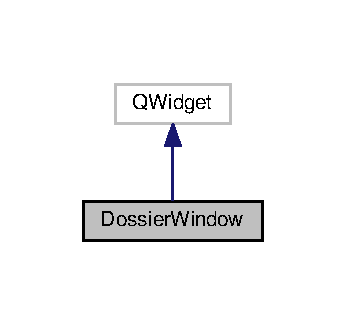
\includegraphics[width=166pt]{class_dossier_window__inherit__graph}
\end{center}
\end{figure}


Collaboration diagram for Dossier\-Window\-:
\nopagebreak
\begin{figure}[H]
\begin{center}
\leavevmode
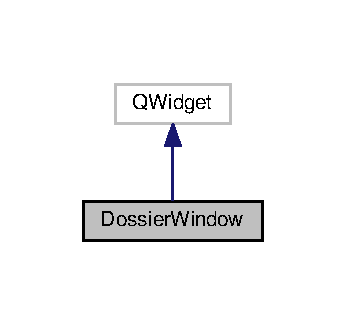
\includegraphics[width=166pt]{class_dossier_window__coll__graph}
\end{center}
\end{figure}
\subsection*{Public Slots}
\begin{DoxyCompactItemize}
\item 
\hypertarget{class_dossier_window_ace55d79178ee85a8cee7203fc555d65b}{void \hyperlink{class_dossier_window_ace55d79178ee85a8cee7203fc555d65b}{sauver} ()}\label{class_dossier_window_ace55d79178ee85a8cee7203fc555d65b}

\begin{DoxyCompactList}\small\item\em Sauvegarde ou ajout d'un dossier. \end{DoxyCompactList}\item 
void \hyperlink{class_dossier_window_a39e3bf3b53585c4e0619f05ef1cb2ba9}{pbsauver\-Enable} ()
\begin{DoxyCompactList}\small\item\em Activation du bouton Sauver. \end{DoxyCompactList}\item 
\hypertarget{class_dossier_window_a585664fe2ceb7da9b4cc3a250b1bcf51}{void \hyperlink{class_dossier_window_a585664fe2ceb7da9b4cc3a250b1bcf51}{rechercher} ()}\label{class_dossier_window_a585664fe2ceb7da9b4cc3a250b1bcf51}

\begin{DoxyCompactList}\small\item\em Recherche d'un dossier existant. \end{DoxyCompactList}\item 
void \hyperlink{class_dossier_window_a7b9d5a609e9838dc9f7eacd72d196e5e}{ajouter\-Form\-Ext} ()
\begin{DoxyCompactList}\small\item\em Ajout d'une formation extérieure. \end{DoxyCompactList}\item 
void \hyperlink{class_dossier_window_a7f5a0e6640ef760f57866c2cd58995a7}{suppr\-Form\-Ext} (int r, int c)
\begin{DoxyCompactList}\small\item\em Suppression d'une formation extérieure. \end{DoxyCompactList}\item 
void \hyperlink{class_dossier_window_a7d408ef7ea4239b0c9a0c7a16446105b}{ajouter\-Semestre} ()
\begin{DoxyCompactList}\small\item\em Ajout d'un semestre. \end{DoxyCompactList}\item 
void \hyperlink{class_dossier_window_a16be820f96498f8f8240ac683541e93a}{suppr\-Semestre} (int r, int c)
\begin{DoxyCompactList}\small\item\em Suppression d'une inscription à un semestre. \end{DoxyCompactList}\item 
void \hyperlink{class_dossier_window_a9a14055702b38bac1ea675a364a24277}{supprimer} ()
\begin{DoxyCompactList}\small\item\em Suppression d'un dossier existant. \end{DoxyCompactList}\end{DoxyCompactItemize}
\subsection*{Public Member Functions}
\begin{DoxyCompactItemize}
\item 
\hypertarget{class_dossier_window_abec87a1dfb4230a3b70a3de10852cfca}{\hyperlink{class_dossier_window_abec87a1dfb4230a3b70a3de10852cfca}{Dossier\-Window} ()}\label{class_dossier_window_abec87a1dfb4230a3b70a3de10852cfca}

\begin{DoxyCompactList}\small\item\em Constructeur de la classe \hyperlink{class_dossier_window}{Dossier\-Window}. \end{DoxyCompactList}\item 
void \hyperlink{class_dossier_window_aa5ef7660c92f59adbadc44bd7aa7f64d}{associer\-Dossier} (\hyperlink{class_dossier}{Dossier} $\ast$d)
\begin{DoxyCompactList}\small\item\em Association d'un dossier aux champs de la fenêtre. \end{DoxyCompactList}\end{DoxyCompactItemize}
\subsection*{Friends}
\begin{DoxyCompactItemize}
\item 
\hypertarget{class_dossier_window_a89f0e38a39f054c26a0ab852f8a79b18}{class {\bfseries Home\-Window}}\label{class_dossier_window_a89f0e38a39f054c26a0ab852f8a79b18}

\end{DoxyCompactItemize}


\subsection{Detailed Description}
Classe pour la fenêtre qui permet de consulter, modifier, ajouter, supprimer un dossier. 

Definition at line 1012 of file U\-T\-Profiler.\-h.



\subsection{Member Function Documentation}
\hypertarget{class_dossier_window_a7b9d5a609e9838dc9f7eacd72d196e5e}{\index{Dossier\-Window@{Dossier\-Window}!ajouter\-Form\-Ext@{ajouter\-Form\-Ext}}
\index{ajouter\-Form\-Ext@{ajouter\-Form\-Ext}!DossierWindow@{Dossier\-Window}}
\subsubsection[{ajouter\-Form\-Ext}]{\setlength{\rightskip}{0pt plus 5cm}void Dossier\-Window\-::ajouter\-Form\-Ext (
\begin{DoxyParamCaption}
{}
\end{DoxyParamCaption}
)\hspace{0.3cm}{\ttfamily [slot]}}}\label{class_dossier_window_a7b9d5a609e9838dc9f7eacd72d196e5e}


Ajout d'une formation extérieure. 

Affiche une fenêtre \hyperlink{class_formation_ext_window}{Formation\-Ext\-Window} pour ajouter une formation extérieure au dossier en cours de visualisation. Cette méthode est appelée par le bouton Ajouter lorsqu'il est cliqué. 

Definition at line 489 of file Dossier\-Window.\-cpp.

\hypertarget{class_dossier_window_a7d408ef7ea4239b0c9a0c7a16446105b}{\index{Dossier\-Window@{Dossier\-Window}!ajouter\-Semestre@{ajouter\-Semestre}}
\index{ajouter\-Semestre@{ajouter\-Semestre}!DossierWindow@{Dossier\-Window}}
\subsubsection[{ajouter\-Semestre}]{\setlength{\rightskip}{0pt plus 5cm}void Dossier\-Window\-::ajouter\-Semestre (
\begin{DoxyParamCaption}
{}
\end{DoxyParamCaption}
)\hspace{0.3cm}{\ttfamily [slot]}}}\label{class_dossier_window_a7d408ef7ea4239b0c9a0c7a16446105b}


Ajout d'un semestre. 

Cette fonction ouvre une \hyperlink{class_semestre_window}{Semestre\-Window} pour pouvoir ajouter une inscription à un \hyperlink{class_u_v}{U\-V} pour le dossier en cours de visualisation. 

Definition at line 526 of file Dossier\-Window.\-cpp.

\hypertarget{class_dossier_window_aa5ef7660c92f59adbadc44bd7aa7f64d}{\index{Dossier\-Window@{Dossier\-Window}!associer\-Dossier@{associer\-Dossier}}
\index{associer\-Dossier@{associer\-Dossier}!DossierWindow@{Dossier\-Window}}
\subsubsection[{associer\-Dossier}]{\setlength{\rightskip}{0pt plus 5cm}void Dossier\-Window\-::associer\-Dossier (
\begin{DoxyParamCaption}
\item[{{\bf Dossier} $\ast$}]{d}
\end{DoxyParamCaption}
)}}\label{class_dossier_window_aa5ef7660c92f59adbadc44bd7aa7f64d}


Association d'un dossier aux champs de la fenêtre. 


\begin{DoxyParams}{Parameters}
{\em d} & \-: le dossier à associer aux champs de la fenêtre \hyperlink{class_dossier_window}{Dossier\-Window} \\
\hline
\end{DoxyParams}


Definition at line 296 of file Dossier\-Window.\-cpp.

\hypertarget{class_dossier_window_a39e3bf3b53585c4e0619f05ef1cb2ba9}{\index{Dossier\-Window@{Dossier\-Window}!pbsauver\-Enable@{pbsauver\-Enable}}
\index{pbsauver\-Enable@{pbsauver\-Enable}!DossierWindow@{Dossier\-Window}}
\subsubsection[{pbsauver\-Enable}]{\setlength{\rightskip}{0pt plus 5cm}void Dossier\-Window\-::pbsauver\-Enable (
\begin{DoxyParamCaption}
{}
\end{DoxyParamCaption}
)\hspace{0.3cm}{\ttfamily [slot]}}}\label{class_dossier_window_a39e3bf3b53585c4e0619f05ef1cb2ba9}


Activation du bouton Sauver. 

Chaque changement au sein de la fenêtre \hyperlink{class_dossier_window}{Dossier\-Window} appelle cette fonction 

Definition at line 286 of file Dossier\-Window.\-cpp.

\hypertarget{class_dossier_window_a7f5a0e6640ef760f57866c2cd58995a7}{\index{Dossier\-Window@{Dossier\-Window}!suppr\-Form\-Ext@{suppr\-Form\-Ext}}
\index{suppr\-Form\-Ext@{suppr\-Form\-Ext}!DossierWindow@{Dossier\-Window}}
\subsubsection[{suppr\-Form\-Ext}]{\setlength{\rightskip}{0pt plus 5cm}void Dossier\-Window\-::suppr\-Form\-Ext (
\begin{DoxyParamCaption}
\item[{int}]{r, }
\item[{int}]{c}
\end{DoxyParamCaption}
)\hspace{0.3cm}{\ttfamily [slot]}}}\label{class_dossier_window_a7f5a0e6640ef760f57866c2cd58995a7}


Suppression d'une formation extérieure. 

Lorsqu'on clique sur une cellule du tableau des formations extérieures, cette fonction est appelée. Si la cellule cliquée appartient à la 6ème colonne du tableau (cellule \char`\"{}\-Supprimer\char`\"{}), alors la ligne est supprimée.


\begin{DoxyParams}{Parameters}
{\em r} & \-: ligne de la cellule cliquée \\
\hline
{\em c} & \-: colonne de la cellule cliquée \\
\hline
\end{DoxyParams}


Definition at line 505 of file Dossier\-Window.\-cpp.

\hypertarget{class_dossier_window_a9a14055702b38bac1ea675a364a24277}{\index{Dossier\-Window@{Dossier\-Window}!supprimer@{supprimer}}
\index{supprimer@{supprimer}!DossierWindow@{Dossier\-Window}}
\subsubsection[{supprimer}]{\setlength{\rightskip}{0pt plus 5cm}void Dossier\-Window\-::supprimer (
\begin{DoxyParamCaption}
{}
\end{DoxyParamCaption}
)\hspace{0.3cm}{\ttfamily [slot]}}}\label{class_dossier_window_a9a14055702b38bac1ea675a364a24277}


Suppression d'un dossier existant. 

Cette fonction supprime un dossier existant et tout ce qui peut lui être relié (Formations extérieures, Semestres, Inscriptions). 

Definition at line 574 of file Dossier\-Window.\-cpp.

\hypertarget{class_dossier_window_a16be820f96498f8f8240ac683541e93a}{\index{Dossier\-Window@{Dossier\-Window}!suppr\-Semestre@{suppr\-Semestre}}
\index{suppr\-Semestre@{suppr\-Semestre}!DossierWindow@{Dossier\-Window}}
\subsubsection[{suppr\-Semestre}]{\setlength{\rightskip}{0pt plus 5cm}void Dossier\-Window\-::suppr\-Semestre (
\begin{DoxyParamCaption}
\item[{int}]{r, }
\item[{int}]{c}
\end{DoxyParamCaption}
)\hspace{0.3cm}{\ttfamily [slot]}}}\label{class_dossier_window_a16be820f96498f8f8240ac683541e93a}


Suppression d'une inscription à un semestre. 

Lorsqu'on clique sur une cellule du tableau des semestres, cette fonction est appelée. Si la cellule cliquée appartient à la 7ème colonne du tableau (cellule \char`\"{}\-Supprimer\char`\"{}), alors la ligne est supprimée.


\begin{DoxyParams}{Parameters}
{\em r} & \-: ligne de la cellule cliquée \\
\hline
{\em c} & \-: colonne de la cellule cliquée \\
\hline
\end{DoxyParams}


Definition at line 542 of file Dossier\-Window.\-cpp.



The documentation for this class was generated from the following files\-:\begin{DoxyCompactItemize}
\item 
\hyperlink{_u_t_profiler_8h}{U\-T\-Profiler.\-h}\item 
\hyperlink{_dossier_window_8cpp}{Dossier\-Window.\-cpp}\end{DoxyCompactItemize}

\hypertarget{class_formation}{\section{Formation Class Reference}
\label{class_formation}\index{Formation@{Formation}}
}


Classe représentant une formation.  




{\ttfamily \#include $<$U\-T\-Profiler.\-h$>$}

\subsection*{Public Member Functions}
\begin{DoxyCompactItemize}
\item 
\hyperlink{class_formation_a845d387195dc1ee6c9da35b7acbd9c75}{Formation} (const Q\-String \&n, const Q\-String \&r, const Q\-String \&t, unsigned int tot, unsigned int cs, unsigned int tm, unsigned int cstm, unsigned int tsh, unsigned int sp)
\begin{DoxyCompactList}\small\item\em Constructeur. \end{DoxyCompactList}\item 
\hyperlink{class_formation_a60c3058dd353550d89183ec529909cb6}{Formation} ()
\begin{DoxyCompactList}\small\item\em Constructeur. \end{DoxyCompactList}\item 
Q\-String \hyperlink{class_formation_ae6a675062709e29c5bfc4f2da7b6ccf2}{get\-Nom} () const 
\begin{DoxyCompactList}\small\item\em Accès en lecture au nom de la formation. \end{DoxyCompactList}\item 
Q\-String \hyperlink{class_formation_ad2e117bb6b0f33dbe35014e5e1904a89}{get\-Responsable} () const 
\begin{DoxyCompactList}\small\item\em Accès en lecture au responsable de la formation. \end{DoxyCompactList}\item 
Q\-String \hyperlink{class_formation_a54006f84fbbd0591527f5036ba8c9b53}{get\-Type} () const 
\begin{DoxyCompactList}\small\item\em Accès en lecture au type de la formation. \end{DoxyCompactList}\item 
\hyperlink{class_u_v}{U\-V} $\ast$ \hyperlink{class_formation_ac0d4ca05416a8f09b1dd011e61a58ce9}{get\-U\-Vs} () const 
\begin{DoxyCompactList}\small\item\em Accès en lecture aux uvs associées à la formation. \end{DoxyCompactList}\item 
unsigned int \hyperlink{class_formation_a68bdd93c31f5aa091729aee3a16061be}{get\-Nb\-Credits\-Tot} () const 
\begin{DoxyCompactList}\small\item\em Accès en lecture au nombre de crédits total requis pour valider la formation. \end{DoxyCompactList}\item 
unsigned int \hyperlink{class_formation_a906d4493dc3de651618e34e7386c1952}{get\-Nb\-Credits\-C\-S} () const 
\begin{DoxyCompactList}\small\item\em Accès en lecture au nombre de crédits C\-S requis pour valider la formation. \end{DoxyCompactList}\item 
unsigned int \hyperlink{class_formation_aa71fe058c17323a5ed1e47714da68657}{get\-Nb\-Credits\-T\-M} () const 
\begin{DoxyCompactList}\small\item\em Accès en lecture au nombre de crédits T\-M requis pour valider la formation. \end{DoxyCompactList}\item 
unsigned int \hyperlink{class_formation_a7be30b6d06a72cb64d1d2163a632be59}{get\-Nb\-Credits\-C\-S\-T\-M} () const 
\begin{DoxyCompactList}\small\item\em Accès en lecture au nombre de crédits C\-S + T\-M requis pour valider la formation. \end{DoxyCompactList}\item 
unsigned int \hyperlink{class_formation_ac7dc1e1c6c8daecd85ae61e71987174b}{get\-Nb\-Credits\-T\-S\-H} () const 
\begin{DoxyCompactList}\small\item\em Accès en lecture au nombre de crédits T\-S\-H requis pour valider la formation. \end{DoxyCompactList}\item 
unsigned int \hyperlink{class_formation_a8c0730ec60fa46b4d5fd1d25ee073741}{get\-Nb\-Credits\-S\-P} () const 
\begin{DoxyCompactList}\small\item\em Accès en lecture au nombre de crédits S\-P requis pour valider la formation. \end{DoxyCompactList}\end{DoxyCompactItemize}


\subsection{Detailed Description}
Classe représentant une formation. 

Definition at line 758 of file U\-T\-Profiler.\-h.



\subsection{Constructor \& Destructor Documentation}
\hypertarget{class_formation_a845d387195dc1ee6c9da35b7acbd9c75}{\index{Formation@{Formation}!Formation@{Formation}}
\index{Formation@{Formation}!Formation@{Formation}}
\subsubsection[{Formation}]{\setlength{\rightskip}{0pt plus 5cm}Formation\-::\-Formation (
\begin{DoxyParamCaption}
\item[{const Q\-String \&}]{n, }
\item[{const Q\-String \&}]{r, }
\item[{const Q\-String \&}]{t, }
\item[{unsigned int}]{tot, }
\item[{unsigned int}]{cs, }
\item[{unsigned int}]{tm, }
\item[{unsigned int}]{cstm, }
\item[{unsigned int}]{tsh, }
\item[{unsigned int}]{sp}
\end{DoxyParamCaption}
)\hspace{0.3cm}{\ttfamily [inline]}}}\label{class_formation_a845d387195dc1ee6c9da35b7acbd9c75}


Constructeur. 

Constructeur de la classe \hyperlink{class_formation}{Formation}


\begin{DoxyParams}{Parameters}
{\em n} & \-: nom de la formation \\
\hline
{\em r} & \-: responsable de la formation \\
\hline
{\em t} & \-: type de la formation \\
\hline
{\em tot} & \-: nombre de crédits total requis pour valider la formation \\
\hline
{\em cs} & \-: nombre de crédits C\-S requis pour valider la formation \\
\hline
{\em tm} & \-: nombre de crédits T\-M requis pour valider la formation \\
\hline
{\em cstm} & \-: nombre de crédits C\-S + T\-M requis pour valider la formation \\
\hline
{\em tsh} & \-: nombre de crédits T\-S\-H requis pour valider la formation \\
\hline
{\em sp} & \-: nombre de crédits S\-P requis pour valider la formation \\
\hline
\end{DoxyParams}


Definition at line 785 of file U\-T\-Profiler.\-h.

\hypertarget{class_formation_a60c3058dd353550d89183ec529909cb6}{\index{Formation@{Formation}!Formation@{Formation}}
\index{Formation@{Formation}!Formation@{Formation}}
\subsubsection[{Formation}]{\setlength{\rightskip}{0pt plus 5cm}Formation\-::\-Formation (
\begin{DoxyParamCaption}
{}
\end{DoxyParamCaption}
)\hspace{0.3cm}{\ttfamily [inline]}}}\label{class_formation_a60c3058dd353550d89183ec529909cb6}


Constructeur. 

Constructeur sans arguments de la classe \hyperlink{class_formation}{Formation} 

Definition at line 792 of file U\-T\-Profiler.\-h.



\subsection{Member Function Documentation}
\hypertarget{class_formation_a906d4493dc3de651618e34e7386c1952}{\index{Formation@{Formation}!get\-Nb\-Credits\-C\-S@{get\-Nb\-Credits\-C\-S}}
\index{get\-Nb\-Credits\-C\-S@{get\-Nb\-Credits\-C\-S}!Formation@{Formation}}
\subsubsection[{get\-Nb\-Credits\-C\-S}]{\setlength{\rightskip}{0pt plus 5cm}unsigned int Formation\-::get\-Nb\-Credits\-C\-S (
\begin{DoxyParamCaption}
{}
\end{DoxyParamCaption}
) const\hspace{0.3cm}{\ttfamily [inline]}}}\label{class_formation_a906d4493dc3de651618e34e7386c1952}


Accès en lecture au nombre de crédits C\-S requis pour valider la formation. 

\begin{DoxyReturn}{Returns}
le nom de crédits C\-S requis pour valider la formation 
\end{DoxyReturn}


Definition at line 834 of file U\-T\-Profiler.\-h.

\hypertarget{class_formation_a7be30b6d06a72cb64d1d2163a632be59}{\index{Formation@{Formation}!get\-Nb\-Credits\-C\-S\-T\-M@{get\-Nb\-Credits\-C\-S\-T\-M}}
\index{get\-Nb\-Credits\-C\-S\-T\-M@{get\-Nb\-Credits\-C\-S\-T\-M}!Formation@{Formation}}
\subsubsection[{get\-Nb\-Credits\-C\-S\-T\-M}]{\setlength{\rightskip}{0pt plus 5cm}unsigned int Formation\-::get\-Nb\-Credits\-C\-S\-T\-M (
\begin{DoxyParamCaption}
{}
\end{DoxyParamCaption}
) const\hspace{0.3cm}{\ttfamily [inline]}}}\label{class_formation_a7be30b6d06a72cb64d1d2163a632be59}


Accès en lecture au nombre de crédits C\-S + T\-M requis pour valider la formation. 

\begin{DoxyReturn}{Returns}
le nom de crédits C\-S + T\-M requis pour valider la formation 
\end{DoxyReturn}


Definition at line 848 of file U\-T\-Profiler.\-h.

\hypertarget{class_formation_a8c0730ec60fa46b4d5fd1d25ee073741}{\index{Formation@{Formation}!get\-Nb\-Credits\-S\-P@{get\-Nb\-Credits\-S\-P}}
\index{get\-Nb\-Credits\-S\-P@{get\-Nb\-Credits\-S\-P}!Formation@{Formation}}
\subsubsection[{get\-Nb\-Credits\-S\-P}]{\setlength{\rightskip}{0pt plus 5cm}unsigned int Formation\-::get\-Nb\-Credits\-S\-P (
\begin{DoxyParamCaption}
{}
\end{DoxyParamCaption}
) const\hspace{0.3cm}{\ttfamily [inline]}}}\label{class_formation_a8c0730ec60fa46b4d5fd1d25ee073741}


Accès en lecture au nombre de crédits S\-P requis pour valider la formation. 

\begin{DoxyReturn}{Returns}
le nom de crédits S\-P requis pour valider la formation 
\end{DoxyReturn}


Definition at line 862 of file U\-T\-Profiler.\-h.

\hypertarget{class_formation_aa71fe058c17323a5ed1e47714da68657}{\index{Formation@{Formation}!get\-Nb\-Credits\-T\-M@{get\-Nb\-Credits\-T\-M}}
\index{get\-Nb\-Credits\-T\-M@{get\-Nb\-Credits\-T\-M}!Formation@{Formation}}
\subsubsection[{get\-Nb\-Credits\-T\-M}]{\setlength{\rightskip}{0pt plus 5cm}unsigned int Formation\-::get\-Nb\-Credits\-T\-M (
\begin{DoxyParamCaption}
{}
\end{DoxyParamCaption}
) const\hspace{0.3cm}{\ttfamily [inline]}}}\label{class_formation_aa71fe058c17323a5ed1e47714da68657}


Accès en lecture au nombre de crédits T\-M requis pour valider la formation. 

\begin{DoxyReturn}{Returns}
le nom de crédits T\-M requis pour valider la formation 
\end{DoxyReturn}


Definition at line 841 of file U\-T\-Profiler.\-h.

\hypertarget{class_formation_a68bdd93c31f5aa091729aee3a16061be}{\index{Formation@{Formation}!get\-Nb\-Credits\-Tot@{get\-Nb\-Credits\-Tot}}
\index{get\-Nb\-Credits\-Tot@{get\-Nb\-Credits\-Tot}!Formation@{Formation}}
\subsubsection[{get\-Nb\-Credits\-Tot}]{\setlength{\rightskip}{0pt plus 5cm}unsigned int Formation\-::get\-Nb\-Credits\-Tot (
\begin{DoxyParamCaption}
{}
\end{DoxyParamCaption}
) const\hspace{0.3cm}{\ttfamily [inline]}}}\label{class_formation_a68bdd93c31f5aa091729aee3a16061be}


Accès en lecture au nombre de crédits total requis pour valider la formation. 

\begin{DoxyReturn}{Returns}
le nom de crédits total requis pour valider la formation 
\end{DoxyReturn}


Definition at line 827 of file U\-T\-Profiler.\-h.

\hypertarget{class_formation_ac7dc1e1c6c8daecd85ae61e71987174b}{\index{Formation@{Formation}!get\-Nb\-Credits\-T\-S\-H@{get\-Nb\-Credits\-T\-S\-H}}
\index{get\-Nb\-Credits\-T\-S\-H@{get\-Nb\-Credits\-T\-S\-H}!Formation@{Formation}}
\subsubsection[{get\-Nb\-Credits\-T\-S\-H}]{\setlength{\rightskip}{0pt plus 5cm}unsigned int Formation\-::get\-Nb\-Credits\-T\-S\-H (
\begin{DoxyParamCaption}
{}
\end{DoxyParamCaption}
) const\hspace{0.3cm}{\ttfamily [inline]}}}\label{class_formation_ac7dc1e1c6c8daecd85ae61e71987174b}


Accès en lecture au nombre de crédits T\-S\-H requis pour valider la formation. 

\begin{DoxyReturn}{Returns}
le nom de crédits T\-S\-H requis pour valider la formation 
\end{DoxyReturn}


Definition at line 855 of file U\-T\-Profiler.\-h.

\hypertarget{class_formation_ae6a675062709e29c5bfc4f2da7b6ccf2}{\index{Formation@{Formation}!get\-Nom@{get\-Nom}}
\index{get\-Nom@{get\-Nom}!Formation@{Formation}}
\subsubsection[{get\-Nom}]{\setlength{\rightskip}{0pt plus 5cm}Q\-String Formation\-::get\-Nom (
\begin{DoxyParamCaption}
{}
\end{DoxyParamCaption}
) const\hspace{0.3cm}{\ttfamily [inline]}}}\label{class_formation_ae6a675062709e29c5bfc4f2da7b6ccf2}


Accès en lecture au nom de la formation. 

\begin{DoxyReturn}{Returns}
le nom de la formation 
\end{DoxyReturn}


Definition at line 799 of file U\-T\-Profiler.\-h.

\hypertarget{class_formation_ad2e117bb6b0f33dbe35014e5e1904a89}{\index{Formation@{Formation}!get\-Responsable@{get\-Responsable}}
\index{get\-Responsable@{get\-Responsable}!Formation@{Formation}}
\subsubsection[{get\-Responsable}]{\setlength{\rightskip}{0pt plus 5cm}Q\-String Formation\-::get\-Responsable (
\begin{DoxyParamCaption}
{}
\end{DoxyParamCaption}
) const\hspace{0.3cm}{\ttfamily [inline]}}}\label{class_formation_ad2e117bb6b0f33dbe35014e5e1904a89}


Accès en lecture au responsable de la formation. 

\begin{DoxyReturn}{Returns}
le responsable de la formation 
\end{DoxyReturn}


Definition at line 806 of file U\-T\-Profiler.\-h.

\hypertarget{class_formation_a54006f84fbbd0591527f5036ba8c9b53}{\index{Formation@{Formation}!get\-Type@{get\-Type}}
\index{get\-Type@{get\-Type}!Formation@{Formation}}
\subsubsection[{get\-Type}]{\setlength{\rightskip}{0pt plus 5cm}Q\-String Formation\-::get\-Type (
\begin{DoxyParamCaption}
{}
\end{DoxyParamCaption}
) const\hspace{0.3cm}{\ttfamily [inline]}}}\label{class_formation_a54006f84fbbd0591527f5036ba8c9b53}


Accès en lecture au type de la formation. 

\begin{DoxyReturn}{Returns}
le type de la formation 
\end{DoxyReturn}


Definition at line 813 of file U\-T\-Profiler.\-h.

\hypertarget{class_formation_ac0d4ca05416a8f09b1dd011e61a58ce9}{\index{Formation@{Formation}!get\-U\-Vs@{get\-U\-Vs}}
\index{get\-U\-Vs@{get\-U\-Vs}!Formation@{Formation}}
\subsubsection[{get\-U\-Vs}]{\setlength{\rightskip}{0pt plus 5cm}{\bf U\-V}$\ast$ Formation\-::get\-U\-Vs (
\begin{DoxyParamCaption}
{}
\end{DoxyParamCaption}
) const\hspace{0.3cm}{\ttfamily [inline]}}}\label{class_formation_ac0d4ca05416a8f09b1dd011e61a58ce9}


Accès en lecture aux uvs associées à la formation. 

\begin{DoxyReturn}{Returns}
les uvs associées à la formation 
\end{DoxyReturn}


Definition at line 820 of file U\-T\-Profiler.\-h.



The documentation for this class was generated from the following file\-:\begin{DoxyCompactItemize}
\item 
\hyperlink{_u_t_profiler_8h}{U\-T\-Profiler.\-h}\end{DoxyCompactItemize}

\hypertarget{class_formation_exterieure}{\section{Formation\-Exterieure Class Reference}
\label{class_formation_exterieure}\index{Formation\-Exterieure@{Formation\-Exterieure}}
}


Classe permettant de décrire une formation extérieure à l'U\-T\-C mais rapportant un certain nombre de crédits par équivalence.  




{\ttfamily \#include $<$U\-T\-Profiler.\-h$>$}

\subsection*{Public Member Functions}
\begin{DoxyCompactItemize}
\item 
\hyperlink{class_formation_exterieure_aaf1f0e33b9e862ccc2b4390e0e2424cd}{Formation\-Exterieure} (const string \&n, const string \&l, unsigned int cs, unsigned int tm, unsigned int tsh, unsigned int sp)
\begin{DoxyCompactList}\small\item\em Constructeur Permet de créer un nouvel objet \hyperlink{class_formation_exterieure}{Formation\-Exterieure} initialisé avec les valeurs passés en paramètre. \end{DoxyCompactList}\item 
\hyperlink{class_formation_exterieure_a64dede0a85be1c33cc477c93cc2a6fcf}{Formation\-Exterieure} (\hyperlink{class_formation_exterieure}{Formation\-Exterieure} \&other)
\begin{DoxyCompactList}\small\item\em Constructeur par recopie Permet de créer un nouvel objet \hyperlink{class_formation_exterieure}{Formation\-Exterieure} identique à un autre objet de la même classe déjà existant. \end{DoxyCompactList}\item 
\hypertarget{class_formation_exterieure_a887fa1d6f08d8ea04b716a9564732586}{\hyperlink{class_formation_exterieure_a887fa1d6f08d8ea04b716a9564732586}{$\sim$\-Formation\-Exterieure} ()}\label{class_formation_exterieure_a887fa1d6f08d8ea04b716a9564732586}

\begin{DoxyCompactList}\small\item\em Destructeur. \end{DoxyCompactList}\item 
string \hyperlink{class_formation_exterieure_a5051dbbbad4ac513e6947f8ec230629b}{get\-Nom} () const 
\begin{DoxyCompactList}\small\item\em Accesseur en lecture du nom de cette formation. \end{DoxyCompactList}\item 
string \hyperlink{class_formation_exterieure_a6ad4f9c7f6a74910dabe2df5be3a2583}{get\-Lieu} () const 
\begin{DoxyCompactList}\small\item\em Accesseur en lecture du lieu de cette formation. \end{DoxyCompactList}\item 
unsigned int \hyperlink{class_formation_exterieure_a10ae8cef1659fc8baec652f568f48008}{get\-Credits\-C\-S} () const 
\begin{DoxyCompactList}\small\item\em Accesseur en lecture du nombre de crédits C\-S validés par cette formation. \end{DoxyCompactList}\item 
unsigned int \hyperlink{class_formation_exterieure_a3ddcc11233eeac50dfe97124f2d7075f}{get\-Credits\-T\-M} () const 
\begin{DoxyCompactList}\small\item\em Accesseur en lecture du nombre de crédits T\-M validés par cette formation. \end{DoxyCompactList}\item 
unsigned int \hyperlink{class_formation_exterieure_abb62cc93c6853995a085d141f79d013f}{get\-Credits\-T\-S\-H} () const 
\begin{DoxyCompactList}\small\item\em Accesseur en lecture du nombre de crédits T\-S\-H validés par cette formation. \end{DoxyCompactList}\item 
unsigned int \hyperlink{class_formation_exterieure_ad9ddc5b335cb8cee7e86c8f83534112c}{get\-Credits\-S\-P} () const 
\begin{DoxyCompactList}\small\item\em Accesseur en lecture du nombre de crédits S\-P validés par cette formation. \end{DoxyCompactList}\item 
void \hyperlink{class_formation_exterieure_ad81e249506fdb1f104ef7474ff600220}{set\-Nom} (const string \&s)
\begin{DoxyCompactList}\small\item\em Accesseur en écriture du nom de cette formation. \end{DoxyCompactList}\item 
void \hyperlink{class_formation_exterieure_a9895b945b46b567648d8d31ede404c05}{set\-Lieu} (const string \&s)
\begin{DoxyCompactList}\small\item\em Accesseur en écriture du nouveau lieu de cette formation. \end{DoxyCompactList}\item 
void \hyperlink{class_formation_exterieure_af96fc3f4bd03c161ba4c09b4363917cd}{set\-Credits\-C\-S} (unsigned int i)
\begin{DoxyCompactList}\small\item\em Accesseur en écriture du nombre de crédits C\-S validés par cette formation. \end{DoxyCompactList}\item 
void \hyperlink{class_formation_exterieure_a2d2930c7cee5a173b2bfefd01136a1bd}{set\-Credits\-T\-M} (unsigned int i)
\begin{DoxyCompactList}\small\item\em Accesseur en écriture du nombre de crédits T\-M validés par cette formation. \end{DoxyCompactList}\item 
void \hyperlink{class_formation_exterieure_a8cd12ed44c76fcb439264e4e0c386de6}{set\-Credits\-T\-S\-H} (unsigned int i)
\begin{DoxyCompactList}\small\item\em Accesseur en écriture du nombre de crédits T\-S\-H validés par cette formation. \end{DoxyCompactList}\item 
void \hyperlink{class_formation_exterieure_a44e44569507d7afbb9c39d20975748b6}{set\-Credits\-S\-P} (unsigned int i)
\begin{DoxyCompactList}\small\item\em Accesseur en écriture du nombre de crédits S\-P validés par cette formation. \end{DoxyCompactList}\end{DoxyCompactItemize}


\subsection{Detailed Description}
Classe permettant de décrire une formation extérieure à l'U\-T\-C mais rapportant un certain nombre de crédits par équivalence. 

Cette classe permet de garder temporairement en mémoire une formation d'un étudiant à l'extérieur de l'U\-T\-C. Cependant, un objet de cette classe n'est que temporaire, puisque toutes nos Formations\-Exterieures sont stockées dans notre Base de Données. 

Definition at line 312 of file U\-T\-Profiler.\-h.



\subsection{Constructor \& Destructor Documentation}
\hypertarget{class_formation_exterieure_aaf1f0e33b9e862ccc2b4390e0e2424cd}{\index{Formation\-Exterieure@{Formation\-Exterieure}!Formation\-Exterieure@{Formation\-Exterieure}}
\index{Formation\-Exterieure@{Formation\-Exterieure}!FormationExterieure@{Formation\-Exterieure}}
\subsubsection[{Formation\-Exterieure}]{\setlength{\rightskip}{0pt plus 5cm}Formation\-Exterieure\-::\-Formation\-Exterieure (
\begin{DoxyParamCaption}
\item[{const string \&}]{n, }
\item[{const string \&}]{l, }
\item[{unsigned int}]{cs, }
\item[{unsigned int}]{tm, }
\item[{unsigned int}]{tsh, }
\item[{unsigned int}]{sp}
\end{DoxyParamCaption}
)\hspace{0.3cm}{\ttfamily [inline]}}}\label{class_formation_exterieure_aaf1f0e33b9e862ccc2b4390e0e2424cd}


Constructeur Permet de créer un nouvel objet \hyperlink{class_formation_exterieure}{Formation\-Exterieure} initialisé avec les valeurs passés en paramètre. 


\begin{DoxyParams}{Parameters}
{\em n} & \-: le nom de cette nouvelle formation \\
\hline
{\em l} & \-: le lieu de cette nouvelle formation \\
\hline
{\em cs} & \-: le nombre de crédits C\-S obtenus par cette nouvelle formation \\
\hline
{\em tm} & \-: le nombre de crédits T\-M obtenus par cette nouvelle formation \\
\hline
{\em tsh} & le nombre de crédits T\-S\-H obtenus par cette nouvelle formation \\
\hline
{\em sp} & le nombre de crédits S\-P obtenus par cette nouvelle formation \\
\hline
\end{DoxyParams}


Definition at line 330 of file U\-T\-Profiler.\-h.

\hypertarget{class_formation_exterieure_a64dede0a85be1c33cc477c93cc2a6fcf}{\index{Formation\-Exterieure@{Formation\-Exterieure}!Formation\-Exterieure@{Formation\-Exterieure}}
\index{Formation\-Exterieure@{Formation\-Exterieure}!FormationExterieure@{Formation\-Exterieure}}
\subsubsection[{Formation\-Exterieure}]{\setlength{\rightskip}{0pt plus 5cm}Formation\-Exterieure\-::\-Formation\-Exterieure (
\begin{DoxyParamCaption}
\item[{{\bf Formation\-Exterieure} \&}]{other}
\end{DoxyParamCaption}
)\hspace{0.3cm}{\ttfamily [inline]}}}\label{class_formation_exterieure_a64dede0a85be1c33cc477c93cc2a6fcf}


Constructeur par recopie Permet de créer un nouvel objet \hyperlink{class_formation_exterieure}{Formation\-Exterieure} identique à un autre objet de la même classe déjà existant. 


\begin{DoxyParams}{Parameters}
{\em other} & \-: l'objet à recopier \\
\hline
\end{DoxyParams}


Definition at line 336 of file U\-T\-Profiler.\-h.



\subsection{Member Function Documentation}
\hypertarget{class_formation_exterieure_a10ae8cef1659fc8baec652f568f48008}{\index{Formation\-Exterieure@{Formation\-Exterieure}!get\-Credits\-C\-S@{get\-Credits\-C\-S}}
\index{get\-Credits\-C\-S@{get\-Credits\-C\-S}!FormationExterieure@{Formation\-Exterieure}}
\subsubsection[{get\-Credits\-C\-S}]{\setlength{\rightskip}{0pt plus 5cm}unsigned int Formation\-Exterieure\-::get\-Credits\-C\-S (
\begin{DoxyParamCaption}
{}
\end{DoxyParamCaption}
) const\hspace{0.3cm}{\ttfamily [inline]}}}\label{class_formation_exterieure_a10ae8cef1659fc8baec652f568f48008}


Accesseur en lecture du nombre de crédits C\-S validés par cette formation. 

\begin{DoxyReturn}{Returns}
Le nombre de crédits C\-S validés par cette formation 
\end{DoxyReturn}


Definition at line 355 of file U\-T\-Profiler.\-h.

\hypertarget{class_formation_exterieure_ad9ddc5b335cb8cee7e86c8f83534112c}{\index{Formation\-Exterieure@{Formation\-Exterieure}!get\-Credits\-S\-P@{get\-Credits\-S\-P}}
\index{get\-Credits\-S\-P@{get\-Credits\-S\-P}!FormationExterieure@{Formation\-Exterieure}}
\subsubsection[{get\-Credits\-S\-P}]{\setlength{\rightskip}{0pt plus 5cm}unsigned int Formation\-Exterieure\-::get\-Credits\-S\-P (
\begin{DoxyParamCaption}
{}
\end{DoxyParamCaption}
) const\hspace{0.3cm}{\ttfamily [inline]}}}\label{class_formation_exterieure_ad9ddc5b335cb8cee7e86c8f83534112c}


Accesseur en lecture du nombre de crédits S\-P validés par cette formation. 

\begin{DoxyReturn}{Returns}
Le nombre de crédits S\-P validés par cette formation 
\end{DoxyReturn}


Definition at line 370 of file U\-T\-Profiler.\-h.

\hypertarget{class_formation_exterieure_a3ddcc11233eeac50dfe97124f2d7075f}{\index{Formation\-Exterieure@{Formation\-Exterieure}!get\-Credits\-T\-M@{get\-Credits\-T\-M}}
\index{get\-Credits\-T\-M@{get\-Credits\-T\-M}!FormationExterieure@{Formation\-Exterieure}}
\subsubsection[{get\-Credits\-T\-M}]{\setlength{\rightskip}{0pt plus 5cm}unsigned int Formation\-Exterieure\-::get\-Credits\-T\-M (
\begin{DoxyParamCaption}
{}
\end{DoxyParamCaption}
) const\hspace{0.3cm}{\ttfamily [inline]}}}\label{class_formation_exterieure_a3ddcc11233eeac50dfe97124f2d7075f}


Accesseur en lecture du nombre de crédits T\-M validés par cette formation. 

\begin{DoxyReturn}{Returns}
Le nombre de crédits T\-M validés par cette formation 
\end{DoxyReturn}


Definition at line 360 of file U\-T\-Profiler.\-h.

\hypertarget{class_formation_exterieure_abb62cc93c6853995a085d141f79d013f}{\index{Formation\-Exterieure@{Formation\-Exterieure}!get\-Credits\-T\-S\-H@{get\-Credits\-T\-S\-H}}
\index{get\-Credits\-T\-S\-H@{get\-Credits\-T\-S\-H}!FormationExterieure@{Formation\-Exterieure}}
\subsubsection[{get\-Credits\-T\-S\-H}]{\setlength{\rightskip}{0pt plus 5cm}unsigned int Formation\-Exterieure\-::get\-Credits\-T\-S\-H (
\begin{DoxyParamCaption}
{}
\end{DoxyParamCaption}
) const\hspace{0.3cm}{\ttfamily [inline]}}}\label{class_formation_exterieure_abb62cc93c6853995a085d141f79d013f}


Accesseur en lecture du nombre de crédits T\-S\-H validés par cette formation. 

\begin{DoxyReturn}{Returns}
Le nombre de crédits T\-S\-H validés par cette formation 
\end{DoxyReturn}


Definition at line 365 of file U\-T\-Profiler.\-h.

\hypertarget{class_formation_exterieure_a6ad4f9c7f6a74910dabe2df5be3a2583}{\index{Formation\-Exterieure@{Formation\-Exterieure}!get\-Lieu@{get\-Lieu}}
\index{get\-Lieu@{get\-Lieu}!FormationExterieure@{Formation\-Exterieure}}
\subsubsection[{get\-Lieu}]{\setlength{\rightskip}{0pt plus 5cm}string Formation\-Exterieure\-::get\-Lieu (
\begin{DoxyParamCaption}
{}
\end{DoxyParamCaption}
) const\hspace{0.3cm}{\ttfamily [inline]}}}\label{class_formation_exterieure_a6ad4f9c7f6a74910dabe2df5be3a2583}


Accesseur en lecture du lieu de cette formation. 

\begin{DoxyReturn}{Returns}
Le lieu de cette formation 
\end{DoxyReturn}


Definition at line 350 of file U\-T\-Profiler.\-h.

\hypertarget{class_formation_exterieure_a5051dbbbad4ac513e6947f8ec230629b}{\index{Formation\-Exterieure@{Formation\-Exterieure}!get\-Nom@{get\-Nom}}
\index{get\-Nom@{get\-Nom}!FormationExterieure@{Formation\-Exterieure}}
\subsubsection[{get\-Nom}]{\setlength{\rightskip}{0pt plus 5cm}string Formation\-Exterieure\-::get\-Nom (
\begin{DoxyParamCaption}
{}
\end{DoxyParamCaption}
) const\hspace{0.3cm}{\ttfamily [inline]}}}\label{class_formation_exterieure_a5051dbbbad4ac513e6947f8ec230629b}


Accesseur en lecture du nom de cette formation. 

\begin{DoxyReturn}{Returns}
Le nom de cette formation 
\end{DoxyReturn}


Definition at line 345 of file U\-T\-Profiler.\-h.

\hypertarget{class_formation_exterieure_af96fc3f4bd03c161ba4c09b4363917cd}{\index{Formation\-Exterieure@{Formation\-Exterieure}!set\-Credits\-C\-S@{set\-Credits\-C\-S}}
\index{set\-Credits\-C\-S@{set\-Credits\-C\-S}!FormationExterieure@{Formation\-Exterieure}}
\subsubsection[{set\-Credits\-C\-S}]{\setlength{\rightskip}{0pt plus 5cm}void Formation\-Exterieure\-::set\-Credits\-C\-S (
\begin{DoxyParamCaption}
\item[{unsigned int}]{i}
\end{DoxyParamCaption}
)\hspace{0.3cm}{\ttfamily [inline]}}}\label{class_formation_exterieure_af96fc3f4bd03c161ba4c09b4363917cd}


Accesseur en écriture du nombre de crédits C\-S validés par cette formation. 


\begin{DoxyParams}{Parameters}
{\em i} & \-: Nouveau nombre de crédits C\-S validés par cette formation \\
\hline
\end{DoxyParams}


Definition at line 385 of file U\-T\-Profiler.\-h.

\hypertarget{class_formation_exterieure_a44e44569507d7afbb9c39d20975748b6}{\index{Formation\-Exterieure@{Formation\-Exterieure}!set\-Credits\-S\-P@{set\-Credits\-S\-P}}
\index{set\-Credits\-S\-P@{set\-Credits\-S\-P}!FormationExterieure@{Formation\-Exterieure}}
\subsubsection[{set\-Credits\-S\-P}]{\setlength{\rightskip}{0pt plus 5cm}void Formation\-Exterieure\-::set\-Credits\-S\-P (
\begin{DoxyParamCaption}
\item[{unsigned int}]{i}
\end{DoxyParamCaption}
)\hspace{0.3cm}{\ttfamily [inline]}}}\label{class_formation_exterieure_a44e44569507d7afbb9c39d20975748b6}


Accesseur en écriture du nombre de crédits S\-P validés par cette formation. 


\begin{DoxyParams}{Parameters}
{\em i} & \-: Nouveau nombre de crédits S\-P validés par cette formation \\
\hline
\end{DoxyParams}


Definition at line 400 of file U\-T\-Profiler.\-h.

\hypertarget{class_formation_exterieure_a2d2930c7cee5a173b2bfefd01136a1bd}{\index{Formation\-Exterieure@{Formation\-Exterieure}!set\-Credits\-T\-M@{set\-Credits\-T\-M}}
\index{set\-Credits\-T\-M@{set\-Credits\-T\-M}!FormationExterieure@{Formation\-Exterieure}}
\subsubsection[{set\-Credits\-T\-M}]{\setlength{\rightskip}{0pt plus 5cm}void Formation\-Exterieure\-::set\-Credits\-T\-M (
\begin{DoxyParamCaption}
\item[{unsigned int}]{i}
\end{DoxyParamCaption}
)\hspace{0.3cm}{\ttfamily [inline]}}}\label{class_formation_exterieure_a2d2930c7cee5a173b2bfefd01136a1bd}


Accesseur en écriture du nombre de crédits T\-M validés par cette formation. 


\begin{DoxyParams}{Parameters}
{\em i} & \-: Nouveau nombre de crédits T\-M validés par cette formation \\
\hline
\end{DoxyParams}


Definition at line 390 of file U\-T\-Profiler.\-h.

\hypertarget{class_formation_exterieure_a8cd12ed44c76fcb439264e4e0c386de6}{\index{Formation\-Exterieure@{Formation\-Exterieure}!set\-Credits\-T\-S\-H@{set\-Credits\-T\-S\-H}}
\index{set\-Credits\-T\-S\-H@{set\-Credits\-T\-S\-H}!FormationExterieure@{Formation\-Exterieure}}
\subsubsection[{set\-Credits\-T\-S\-H}]{\setlength{\rightskip}{0pt plus 5cm}void Formation\-Exterieure\-::set\-Credits\-T\-S\-H (
\begin{DoxyParamCaption}
\item[{unsigned int}]{i}
\end{DoxyParamCaption}
)\hspace{0.3cm}{\ttfamily [inline]}}}\label{class_formation_exterieure_a8cd12ed44c76fcb439264e4e0c386de6}


Accesseur en écriture du nombre de crédits T\-S\-H validés par cette formation. 


\begin{DoxyParams}{Parameters}
{\em i} & \-: Nouveau nombre de crédits T\-S\-H validés par cette formation \\
\hline
\end{DoxyParams}


Definition at line 395 of file U\-T\-Profiler.\-h.

\hypertarget{class_formation_exterieure_a9895b945b46b567648d8d31ede404c05}{\index{Formation\-Exterieure@{Formation\-Exterieure}!set\-Lieu@{set\-Lieu}}
\index{set\-Lieu@{set\-Lieu}!FormationExterieure@{Formation\-Exterieure}}
\subsubsection[{set\-Lieu}]{\setlength{\rightskip}{0pt plus 5cm}void Formation\-Exterieure\-::set\-Lieu (
\begin{DoxyParamCaption}
\item[{const string \&}]{s}
\end{DoxyParamCaption}
)\hspace{0.3cm}{\ttfamily [inline]}}}\label{class_formation_exterieure_a9895b945b46b567648d8d31ede404c05}


Accesseur en écriture du nouveau lieu de cette formation. 


\begin{DoxyParams}{Parameters}
{\em s} & \-: Le nouveau lieu de cette formation \\
\hline
\end{DoxyParams}


Definition at line 380 of file U\-T\-Profiler.\-h.

\hypertarget{class_formation_exterieure_ad81e249506fdb1f104ef7474ff600220}{\index{Formation\-Exterieure@{Formation\-Exterieure}!set\-Nom@{set\-Nom}}
\index{set\-Nom@{set\-Nom}!FormationExterieure@{Formation\-Exterieure}}
\subsubsection[{set\-Nom}]{\setlength{\rightskip}{0pt plus 5cm}void Formation\-Exterieure\-::set\-Nom (
\begin{DoxyParamCaption}
\item[{const string \&}]{s}
\end{DoxyParamCaption}
)\hspace{0.3cm}{\ttfamily [inline]}}}\label{class_formation_exterieure_ad81e249506fdb1f104ef7474ff600220}


Accesseur en écriture du nom de cette formation. 


\begin{DoxyParams}{Parameters}
{\em s} & \-: Le nouveau nom de cette formation \\
\hline
\end{DoxyParams}


Definition at line 375 of file U\-T\-Profiler.\-h.



The documentation for this class was generated from the following file\-:\begin{DoxyCompactItemize}
\item 
\hyperlink{_u_t_profiler_8h}{U\-T\-Profiler.\-h}\end{DoxyCompactItemize}

\hypertarget{class_formation_ext_window}{\section{Formation\-Ext\-Window Class Reference}
\label{class_formation_ext_window}\index{Formation\-Ext\-Window@{Formation\-Ext\-Window}}
}


Classe qui permet d'ajouter une formation extérieure à un login existant.  




{\ttfamily \#include $<$U\-T\-Profiler.\-h$>$}



Inheritance diagram for Formation\-Ext\-Window\-:
\nopagebreak
\begin{figure}[H]
\begin{center}
\leavevmode
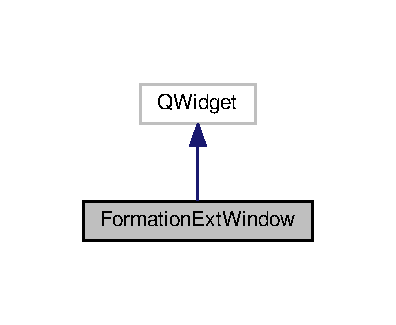
\includegraphics[width=190pt]{class_formation_ext_window__inherit__graph}
\end{center}
\end{figure}


Collaboration diagram for Formation\-Ext\-Window\-:
\nopagebreak
\begin{figure}[H]
\begin{center}
\leavevmode
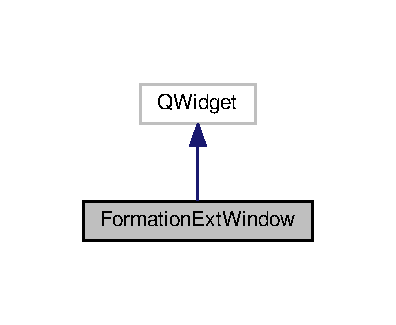
\includegraphics[width=190pt]{class_formation_ext_window__coll__graph}
\end{center}
\end{figure}
\subsection*{Public Slots}
\begin{DoxyCompactItemize}
\item 
void \hyperlink{class_formation_ext_window_a3125317a28eca3c336bd85318c9e335e}{ajouter} ()
\begin{DoxyCompactList}\small\item\em Ajout d'une formation extérieure. \end{DoxyCompactList}\end{DoxyCompactItemize}
\subsection*{Public Member Functions}
\begin{DoxyCompactItemize}
\item 
\hyperlink{class_formation_ext_window_a54279c13d4ad9a40f27954ea348b739a}{Formation\-Ext\-Window} (const Q\-String \&l)
\begin{DoxyCompactList}\small\item\em Constructeur de \hyperlink{class_formation_ext_window}{Formation\-Ext\-Window}. \end{DoxyCompactList}\item 
Q\-String \hyperlink{class_formation_ext_window_ad72d2207a8d27dac54431963e51057b4}{get\-Login} () const 
\begin{DoxyCompactList}\small\item\em Accès en lecture au login. \end{DoxyCompactList}\end{DoxyCompactItemize}


\subsection{Detailed Description}
Classe qui permet d'ajouter une formation extérieure à un login existant. 

Definition at line 1083 of file U\-T\-Profiler.\-h.



\subsection{Constructor \& Destructor Documentation}
\hypertarget{class_formation_ext_window_a54279c13d4ad9a40f27954ea348b739a}{\index{Formation\-Ext\-Window@{Formation\-Ext\-Window}!Formation\-Ext\-Window@{Formation\-Ext\-Window}}
\index{Formation\-Ext\-Window@{Formation\-Ext\-Window}!FormationExtWindow@{Formation\-Ext\-Window}}
\subsubsection[{Formation\-Ext\-Window}]{\setlength{\rightskip}{0pt plus 5cm}Formation\-Ext\-Window\-::\-Formation\-Ext\-Window (
\begin{DoxyParamCaption}
\item[{const Q\-String \&}]{l}
\end{DoxyParamCaption}
)}}\label{class_formation_ext_window_a54279c13d4ad9a40f27954ea348b739a}


Constructeur de \hyperlink{class_formation_ext_window}{Formation\-Ext\-Window}. 

Affiche une fenêtre pour ajouter une formation extérieure au dossier en cours de visualisation.


\begin{DoxyParams}{Parameters}
{\em l} & \-: login du dossier auquel on souhaite ajouter une formation extérieure \\
\hline
\end{DoxyParams}


Definition at line 634 of file Dossier\-Window.\-cpp.



\subsection{Member Function Documentation}
\hypertarget{class_formation_ext_window_a3125317a28eca3c336bd85318c9e335e}{\index{Formation\-Ext\-Window@{Formation\-Ext\-Window}!ajouter@{ajouter}}
\index{ajouter@{ajouter}!FormationExtWindow@{Formation\-Ext\-Window}}
\subsubsection[{ajouter}]{\setlength{\rightskip}{0pt plus 5cm}void Formation\-Ext\-Window\-::ajouter (
\begin{DoxyParamCaption}
{}
\end{DoxyParamCaption}
)\hspace{0.3cm}{\ttfamily [slot]}}}\label{class_formation_ext_window_a3125317a28eca3c336bd85318c9e335e}


Ajout d'une formation extérieure. 

Fonction appelée lorsque l'utilisateur clique sur le bouton Ajouter. 

Definition at line 692 of file Dossier\-Window.\-cpp.

\hypertarget{class_formation_ext_window_ad72d2207a8d27dac54431963e51057b4}{\index{Formation\-Ext\-Window@{Formation\-Ext\-Window}!get\-Login@{get\-Login}}
\index{get\-Login@{get\-Login}!FormationExtWindow@{Formation\-Ext\-Window}}
\subsubsection[{get\-Login}]{\setlength{\rightskip}{0pt plus 5cm}Q\-String Formation\-Ext\-Window\-::get\-Login (
\begin{DoxyParamCaption}
{}
\end{DoxyParamCaption}
) const\hspace{0.3cm}{\ttfamily [inline]}}}\label{class_formation_ext_window_ad72d2207a8d27dac54431963e51057b4}


Accès en lecture au login. 

\begin{DoxyReturn}{Returns}
l'attribut login 
\end{DoxyReturn}


Definition at line 1118 of file U\-T\-Profiler.\-h.



The documentation for this class was generated from the following files\-:\begin{DoxyCompactItemize}
\item 
\hyperlink{_u_t_profiler_8h}{U\-T\-Profiler.\-h}\item 
\hyperlink{_dossier_window_8cpp}{Dossier\-Window.\-cpp}\end{DoxyCompactItemize}

\hypertarget{class_formation_window}{\section{Formation\-Window Class Reference}
\label{class_formation_window}\index{Formation\-Window@{Formation\-Window}}
}


Classe de la fenêtre pour la gestion des formations.  




{\ttfamily \#include $<$U\-T\-Profiler.\-h$>$}



Inheritance diagram for Formation\-Window\-:
\nopagebreak
\begin{figure}[H]
\begin{center}
\leavevmode
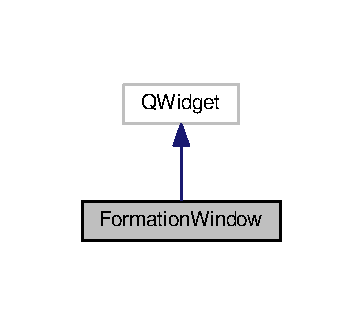
\includegraphics[width=174pt]{class_formation_window__inherit__graph}
\end{center}
\end{figure}


Collaboration diagram for Formation\-Window\-:
\nopagebreak
\begin{figure}[H]
\begin{center}
\leavevmode
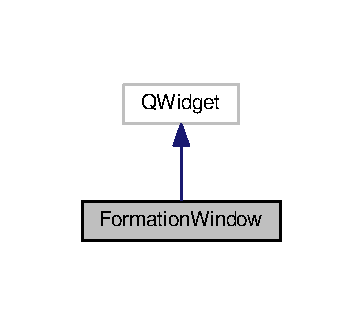
\includegraphics[width=174pt]{class_formation_window__coll__graph}
\end{center}
\end{figure}
\subsection*{Public Slots}
\begin{DoxyCompactItemize}
\item 
void \hyperlink{class_formation_window_afe595a0a344e7884a2199d49685b72c8}{setenabled} ()
\begin{DoxyCompactList}\small\item\em Activation du bouton Sauver. \end{DoxyCompactList}\item 
\hypertarget{class_formation_window_ab1bb1608745c98b9fb3d26df1dcd07cf}{void \hyperlink{class_formation_window_ab1bb1608745c98b9fb3d26df1dcd07cf}{rechercher} ()}\label{class_formation_window_ab1bb1608745c98b9fb3d26df1dcd07cf}

\begin{DoxyCompactList}\small\item\em Recherche d'une formation existante. \end{DoxyCompactList}\item 
void \hyperlink{class_formation_window_aa1a7bd64e46219b7751dc32322882f5e}{nouveau} ()
\begin{DoxyCompactList}\small\item\em Ajout d'une nouvelle formation. \end{DoxyCompactList}\item 
\hypertarget{class_formation_window_a5c6f76c574a7eb28810e718ce88faa40}{void \hyperlink{class_formation_window_a5c6f76c574a7eb28810e718ce88faa40}{supprimer} ()}\label{class_formation_window_a5c6f76c574a7eb28810e718ce88faa40}

\begin{DoxyCompactList}\small\item\em Suppression d'une formation existante. \end{DoxyCompactList}\item 
\hypertarget{class_formation_window_a9c6fb184cf96a862bd13cb30c17131d1}{void \hyperlink{class_formation_window_a9c6fb184cf96a862bd13cb30c17131d1}{sauver} ()}\label{class_formation_window_a9c6fb184cf96a862bd13cb30c17131d1}

\begin{DoxyCompactList}\small\item\em Sauvegarde d'une formation existante. \end{DoxyCompactList}\item 
void \hyperlink{class_formation_window_a6efc5f1397dda264a7044d909d8afeab}{sauveruv} (int r, int c)
\begin{DoxyCompactList}\small\item\em Sauvegarde ou suppression d'une uv associée. \end{DoxyCompactList}\item 
void \hyperlink{class_formation_window_a58b7866f8ef1242df39e33891bdd3dcc}{ajouteruv} ()
\begin{DoxyCompactList}\small\item\em Ajout d'une uv associée à une formation. \end{DoxyCompactList}\item 
void \hyperlink{class_formation_window_a9c5b19cd30fb56ddef12734a2ed68087}{sauverfil} (int r, int c)
\begin{DoxyCompactList}\small\item\em Sauvegarde ou suppression d'une filière associée à une branche. \end{DoxyCompactList}\item 
void \hyperlink{class_formation_window_a315bc4d9e13e94e0c03a778941afe0ea}{ajouterfil} ()
\begin{DoxyCompactList}\small\item\em Ajout d'une filière associée à une branche. \end{DoxyCompactList}\end{DoxyCompactItemize}
\subsection*{Public Member Functions}
\begin{DoxyCompactItemize}
\item 
\hypertarget{class_formation_window_aa440700b3980344aa7099bd3767c9b55}{\hyperlink{class_formation_window_aa440700b3980344aa7099bd3767c9b55}{Formation\-Window} ()}\label{class_formation_window_aa440700b3980344aa7099bd3767c9b55}

\begin{DoxyCompactList}\small\item\em Constructeur de \hyperlink{class_formation_window}{Formation\-Window}. \end{DoxyCompactList}\item 
void \hyperlink{class_formation_window_a0b0eefb2086fee1ac8250cd1aa1eacc5}{associer\-Formation} (\hyperlink{class_formation}{Formation} $\ast$formation)
\begin{DoxyCompactList}\small\item\em Association d'une formation aux champs de la fenêtre. \end{DoxyCompactList}\end{DoxyCompactItemize}
\subsection*{Friends}
\begin{DoxyCompactItemize}
\item 
\hypertarget{class_formation_window_a89f0e38a39f054c26a0ab852f8a79b18}{class {\bfseries Home\-Window}}\label{class_formation_window_a89f0e38a39f054c26a0ab852f8a79b18}

\end{DoxyCompactItemize}


\subsection{Detailed Description}
Classe de la fenêtre pour la gestion des formations. 

Definition at line 1195 of file U\-T\-Profiler.\-h.



\subsection{Member Function Documentation}
\hypertarget{class_formation_window_a315bc4d9e13e94e0c03a778941afe0ea}{\index{Formation\-Window@{Formation\-Window}!ajouterfil@{ajouterfil}}
\index{ajouterfil@{ajouterfil}!FormationWindow@{Formation\-Window}}
\subsubsection[{ajouterfil}]{\setlength{\rightskip}{0pt plus 5cm}void Formation\-Window\-::ajouterfil (
\begin{DoxyParamCaption}
{}
\end{DoxyParamCaption}
)\hspace{0.3cm}{\ttfamily [slot]}}}\label{class_formation_window_a315bc4d9e13e94e0c03a778941afe0ea}


Ajout d'une filière associée à une branche. 

Cette fonction affiche une \hyperlink{class_associer_filiere_window}{Associer\-Filiere\-Window} lorsque l'utilisateur clique sur Ajouter. 

Definition at line 595 of file Formation\-Window.\-cpp.

\hypertarget{class_formation_window_a58b7866f8ef1242df39e33891bdd3dcc}{\index{Formation\-Window@{Formation\-Window}!ajouteruv@{ajouteruv}}
\index{ajouteruv@{ajouteruv}!FormationWindow@{Formation\-Window}}
\subsubsection[{ajouteruv}]{\setlength{\rightskip}{0pt plus 5cm}void Formation\-Window\-::ajouteruv (
\begin{DoxyParamCaption}
{}
\end{DoxyParamCaption}
)\hspace{0.3cm}{\ttfamily [slot]}}}\label{class_formation_window_a58b7866f8ef1242df39e33891bdd3dcc}


Ajout d'une uv associée à une formation. 

Cette fonction affiche une \hyperlink{class_associer_u_v_window}{Associer\-U\-V\-Window} lorsque l'utilisateur clique sur Ajouter. 

Definition at line 582 of file Formation\-Window.\-cpp.

\hypertarget{class_formation_window_a0b0eefb2086fee1ac8250cd1aa1eacc5}{\index{Formation\-Window@{Formation\-Window}!associer\-Formation@{associer\-Formation}}
\index{associer\-Formation@{associer\-Formation}!FormationWindow@{Formation\-Window}}
\subsubsection[{associer\-Formation}]{\setlength{\rightskip}{0pt plus 5cm}void Formation\-Window\-::associer\-Formation (
\begin{DoxyParamCaption}
\item[{{\bf Formation} $\ast$}]{newformation}
\end{DoxyParamCaption}
)}}\label{class_formation_window_a0b0eefb2086fee1ac8250cd1aa1eacc5}


Association d'une formation aux champs de la fenêtre. 


\begin{DoxyParams}{Parameters}
{\em newformation} & \-: la formation à associer aux champs de la fenêtre \hyperlink{class_dossier_window}{Dossier\-Window} \\
\hline
\end{DoxyParams}


Definition at line 158 of file Formation\-Window.\-cpp.

\hypertarget{class_formation_window_aa1a7bd64e46219b7751dc32322882f5e}{\index{Formation\-Window@{Formation\-Window}!nouveau@{nouveau}}
\index{nouveau@{nouveau}!FormationWindow@{Formation\-Window}}
\subsubsection[{nouveau}]{\setlength{\rightskip}{0pt plus 5cm}void Formation\-Window\-::nouveau (
\begin{DoxyParamCaption}
{}
\end{DoxyParamCaption}
)\hspace{0.3cm}{\ttfamily [slot]}}}\label{class_formation_window_aa1a7bd64e46219b7751dc32322882f5e}


Ajout d'une nouvelle formation. 

Cette fonction est appelée lorsque l'utilisateur clique sur le bouton Nouveau. Elle ouvre une fenêtre \hyperlink{class_new_formation_window}{New\-Formation\-Window}. 

Definition at line 309 of file Formation\-Window.\-cpp.

\hypertarget{class_formation_window_a9c5b19cd30fb56ddef12734a2ed68087}{\index{Formation\-Window@{Formation\-Window}!sauverfil@{sauverfil}}
\index{sauverfil@{sauverfil}!FormationWindow@{Formation\-Window}}
\subsubsection[{sauverfil}]{\setlength{\rightskip}{0pt plus 5cm}void Formation\-Window\-::sauverfil (
\begin{DoxyParamCaption}
\item[{int}]{r, }
\item[{int}]{c}
\end{DoxyParamCaption}
)\hspace{0.3cm}{\ttfamily [slot]}}}\label{class_formation_window_a9c5b19cd30fb56ddef12734a2ed68087}


Sauvegarde ou suppression d'une filière associée à une branche. 

Cette fonction est appelée lorsqu'une cellule du tableau des filières associées est cliquée. Selon la cellule cliquée, cette fonction enregistre les modifications apportées à une filière, ou la supprime de la table Association\-Branche\-Filiere.


\begin{DoxyParams}{Parameters}
{\em r} & \-: ligne de la cellule cliquée. \\
\hline
{\em c} & \-: colonne de la cellule cliquée. \\
\hline
\end{DoxyParams}


Definition at line 474 of file Formation\-Window.\-cpp.

\hypertarget{class_formation_window_a6efc5f1397dda264a7044d909d8afeab}{\index{Formation\-Window@{Formation\-Window}!sauveruv@{sauveruv}}
\index{sauveruv@{sauveruv}!FormationWindow@{Formation\-Window}}
\subsubsection[{sauveruv}]{\setlength{\rightskip}{0pt plus 5cm}void Formation\-Window\-::sauveruv (
\begin{DoxyParamCaption}
\item[{int}]{r, }
\item[{int}]{c}
\end{DoxyParamCaption}
)\hspace{0.3cm}{\ttfamily [slot]}}}\label{class_formation_window_a6efc5f1397dda264a7044d909d8afeab}


Sauvegarde ou suppression d'une uv associée. 

Cette fonction est appelée lorsqu'une cellule du tableau des uv associées est cliquée. Selon la cellule cliquée, cette fonction enregistre les modifications apportées à une uv, ou la supprime de la table Association\-Formation\-U\-V.


\begin{DoxyParams}{Parameters}
{\em r} & \-: ligne de la cellule cliquée. \\
\hline
{\em c} & \-: colonne de la cellule cliquée. \\
\hline
\end{DoxyParams}


Definition at line 423 of file Formation\-Window.\-cpp.

\hypertarget{class_formation_window_afe595a0a344e7884a2199d49685b72c8}{\index{Formation\-Window@{Formation\-Window}!setenabled@{setenabled}}
\index{setenabled@{setenabled}!FormationWindow@{Formation\-Window}}
\subsubsection[{setenabled}]{\setlength{\rightskip}{0pt plus 5cm}void Formation\-Window\-::setenabled (
\begin{DoxyParamCaption}
{}
\end{DoxyParamCaption}
)\hspace{0.3cm}{\ttfamily [slot]}}}\label{class_formation_window_afe595a0a344e7884a2199d49685b72c8}


Activation du bouton Sauver. 

Cette fonction est appelée lorsqu'un champ de la fenêtre est modifié. 

Definition at line 265 of file Formation\-Window.\-cpp.



The documentation for this class was generated from the following files\-:\begin{DoxyCompactItemize}
\item 
\hyperlink{_u_t_profiler_8h}{U\-T\-Profiler.\-h}\item 
\hyperlink{_formation_window_8cpp}{Formation\-Window.\-cpp}\end{DoxyCompactItemize}

\hypertarget{class_home_window}{\section{Home\-Window Class Reference}
\label{class_home_window}\index{Home\-Window@{Home\-Window}}
}


Classe de la fenêtre d'accueil de U\-T\-Profiler.  




{\ttfamily \#include $<$U\-T\-Profiler.\-h$>$}



Inheritance diagram for Home\-Window\-:
\nopagebreak
\begin{figure}[H]
\begin{center}
\leavevmode
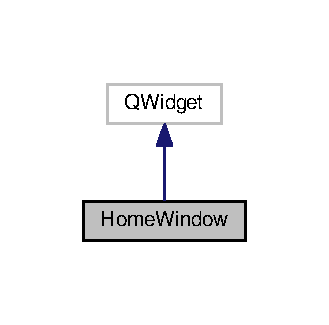
\includegraphics[width=158pt]{class_home_window__inherit__graph}
\end{center}
\end{figure}


Collaboration diagram for Home\-Window\-:
\nopagebreak
\begin{figure}[H]
\begin{center}
\leavevmode
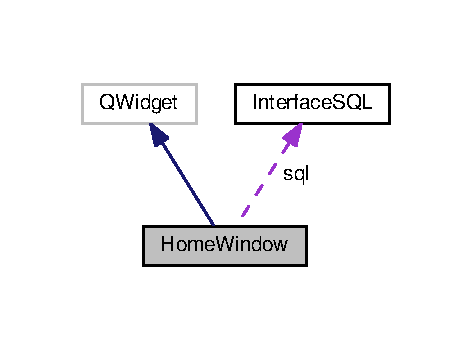
\includegraphics[width=227pt]{class_home_window__coll__graph}
\end{center}
\end{figure}
\subsection*{Public Member Functions}
\begin{DoxyCompactItemize}
\item 
\hypertarget{class_home_window_ae2508edddb566e636a11fa47997acfec}{\hyperlink{class_home_window_ae2508edddb566e636a11fa47997acfec}{Home\-Window} ()}\label{class_home_window_ae2508edddb566e636a11fa47997acfec}

\begin{DoxyCompactList}\small\item\em Constructeur de \hyperlink{class_home_window}{Home\-Window}. \end{DoxyCompactList}\end{DoxyCompactItemize}
\subsection*{Public Attributes}
\begin{DoxyCompactItemize}
\item 
\hypertarget{class_home_window_a89ddfafe9888e97fa39a62e798c38263}{\hyperlink{class_interface_s_q_l}{Interface\-S\-Q\-L} $\ast$ {\bfseries sql}}\label{class_home_window_a89ddfafe9888e97fa39a62e798c38263}

\end{DoxyCompactItemize}


\subsection{Detailed Description}
Classe de la fenêtre d'accueil de U\-T\-Profiler. 

Definition at line 1393 of file U\-T\-Profiler.\-h.



The documentation for this class was generated from the following files\-:\begin{DoxyCompactItemize}
\item 
\hyperlink{_u_t_profiler_8h}{U\-T\-Profiler.\-h}\item 
\hyperlink{_home_window_8cpp}{Home\-Window.\-cpp}\end{DoxyCompactItemize}

\hypertarget{class_inscription}{\section{Inscription Class Reference}
\label{class_inscription}\index{Inscription@{Inscription}}
}


Classe permettant de décrire l'inscription d'un étudiant à une \hyperlink{class_u_v}{U\-V} de l'U\-T\-C.  




{\ttfamily \#include $<$U\-T\-Profiler.\-h$>$}

\subsection*{Public Member Functions}
\begin{DoxyCompactItemize}
\item 
\hypertarget{class_inscription_a1eb6ac1e090dd05570321829e959d75f}{\hyperlink{class_inscription_a1eb6ac1e090dd05570321829e959d75f}{Inscription} ()}\label{class_inscription_a1eb6ac1e090dd05570321829e959d75f}

\begin{DoxyCompactList}\small\item\em Constructeur vide Crée un nouvel objet \hyperlink{class_inscription}{Inscription} non initialisé \end{DoxyCompactList}\item 
\hypertarget{class_inscription_abe0df05b5f2034ae418ae476f7db9ee7}{\hyperlink{class_inscription_abe0df05b5f2034ae418ae476f7db9ee7}{$\sim$\-Inscription} ()}\label{class_inscription_abe0df05b5f2034ae418ae476f7db9ee7}

\begin{DoxyCompactList}\small\item\em Destructeur. \end{DoxyCompactList}\item 
string \hyperlink{class_inscription_a139f354cf118455ab7bb561f656fa691}{get\-U\-V} () const 
\begin{DoxyCompactList}\small\item\em Accesseur en lecture pour le code de l'\hyperlink{class_u_v}{U\-V} auquel l'étudiant est inscrit. \end{DoxyCompactList}\item 
\hyperlink{_u_t_profiler_8h_a89d667cddcff9ee818f60f3d9c6ac987}{Resultat} \hyperlink{class_inscription_a4c38354111c534ed4809da99caf3822f}{get\-Resultat} () const 
\begin{DoxyCompactList}\small\item\em Accesseur en lecture pour le statut de la validation de l'\hyperlink{class_u_v}{U\-V} par l'étudiant. \end{DoxyCompactList}\item 
string \hyperlink{class_inscription_a195d9639695dc78b79f03abd89ce06a1}{get\-Login} () const 
\begin{DoxyCompactList}\small\item\em Accesseur en lecture pour le login de l'étudiant. \end{DoxyCompactList}\item 
void \hyperlink{class_inscription_a33550fc27d9a7a41c7291fe98c730973}{set\-Uv} (const string \&s)
\begin{DoxyCompactList}\small\item\em Accesseur en écriture pour le code de l'\hyperlink{class_u_v}{U\-V} dont il est question. \end{DoxyCompactList}\item 
void \hyperlink{class_inscription_aa957f1dab96c32d59dff404c054f9ad1}{set\-Resultat} (\hyperlink{_u_t_profiler_8h_a89d667cddcff9ee818f60f3d9c6ac987}{Resultat} \&r)
\begin{DoxyCompactList}\small\item\em Accesseur en écriture pour le statut de la validation de l'\hyperlink{class_u_v}{U\-V} en question. \end{DoxyCompactList}\item 
void \hyperlink{class_inscription_a9e1b9d1dd5732ba9e18160e806bfec50}{set\-Login} (const string \&l)
\begin{DoxyCompactList}\small\item\em Accesseur en écriture pour le login de l'étudiant concerné \end{DoxyCompactList}\end{DoxyCompactItemize}


\subsection{Detailed Description}
Classe permettant de décrire l'inscription d'un étudiant à une \hyperlink{class_u_v}{U\-V} de l'U\-T\-C. 

Cette classe permet de garder temporairement en mémoire l'inscription d'un étudiant à une \hyperlink{class_u_v}{U\-V}. Cependant, un objet de cette classe n'est que temporaire, puisque toutes nos Inscriptions sont stockées dans notre Base de Données. 

Definition at line 260 of file U\-T\-Profiler.\-h.



\subsection{Member Function Documentation}
\hypertarget{class_inscription_a195d9639695dc78b79f03abd89ce06a1}{\index{Inscription@{Inscription}!get\-Login@{get\-Login}}
\index{get\-Login@{get\-Login}!Inscription@{Inscription}}
\subsubsection[{get\-Login}]{\setlength{\rightskip}{0pt plus 5cm}string Inscription\-::get\-Login (
\begin{DoxyParamCaption}
{}
\end{DoxyParamCaption}
) const\hspace{0.3cm}{\ttfamily [inline]}}}\label{class_inscription_a195d9639695dc78b79f03abd89ce06a1}


Accesseur en lecture pour le login de l'étudiant. 

\begin{DoxyReturn}{Returns}
Le login de l'étudiant en question 
\end{DoxyReturn}


Definition at line 288 of file U\-T\-Profiler.\-h.

\hypertarget{class_inscription_a4c38354111c534ed4809da99caf3822f}{\index{Inscription@{Inscription}!get\-Resultat@{get\-Resultat}}
\index{get\-Resultat@{get\-Resultat}!Inscription@{Inscription}}
\subsubsection[{get\-Resultat}]{\setlength{\rightskip}{0pt plus 5cm}{\bf Resultat} Inscription\-::get\-Resultat (
\begin{DoxyParamCaption}
{}
\end{DoxyParamCaption}
) const\hspace{0.3cm}{\ttfamily [inline]}}}\label{class_inscription_a4c38354111c534ed4809da99caf3822f}


Accesseur en lecture pour le statut de la validation de l'\hyperlink{class_u_v}{U\-V} par l'étudiant. 

\begin{DoxyReturn}{Returns}
Le statut de la validation de cette \hyperlink{class_u_v}{U\-V} 
\end{DoxyReturn}


Definition at line 283 of file U\-T\-Profiler.\-h.

\hypertarget{class_inscription_a139f354cf118455ab7bb561f656fa691}{\index{Inscription@{Inscription}!get\-U\-V@{get\-U\-V}}
\index{get\-U\-V@{get\-U\-V}!Inscription@{Inscription}}
\subsubsection[{get\-U\-V}]{\setlength{\rightskip}{0pt plus 5cm}string Inscription\-::get\-U\-V (
\begin{DoxyParamCaption}
{}
\end{DoxyParamCaption}
) const\hspace{0.3cm}{\ttfamily [inline]}}}\label{class_inscription_a139f354cf118455ab7bb561f656fa691}


Accesseur en lecture pour le code de l'\hyperlink{class_u_v}{U\-V} auquel l'étudiant est inscrit. 

\begin{DoxyReturn}{Returns}
Le code de l'\hyperlink{class_u_v}{U\-V} en question 
\end{DoxyReturn}


Definition at line 278 of file U\-T\-Profiler.\-h.

\hypertarget{class_inscription_a9e1b9d1dd5732ba9e18160e806bfec50}{\index{Inscription@{Inscription}!set\-Login@{set\-Login}}
\index{set\-Login@{set\-Login}!Inscription@{Inscription}}
\subsubsection[{set\-Login}]{\setlength{\rightskip}{0pt plus 5cm}void Inscription\-::set\-Login (
\begin{DoxyParamCaption}
\item[{const string \&}]{l}
\end{DoxyParamCaption}
)\hspace{0.3cm}{\ttfamily [inline]}}}\label{class_inscription_a9e1b9d1dd5732ba9e18160e806bfec50}


Accesseur en écriture pour le login de l'étudiant concerné 


\begin{DoxyParams}{Parameters}
{\em l} & \-: le login du nouvel étudiant lié à cette inscription \\
\hline
\end{DoxyParams}


Definition at line 303 of file U\-T\-Profiler.\-h.

\hypertarget{class_inscription_aa957f1dab96c32d59dff404c054f9ad1}{\index{Inscription@{Inscription}!set\-Resultat@{set\-Resultat}}
\index{set\-Resultat@{set\-Resultat}!Inscription@{Inscription}}
\subsubsection[{set\-Resultat}]{\setlength{\rightskip}{0pt plus 5cm}void Inscription\-::set\-Resultat (
\begin{DoxyParamCaption}
\item[{{\bf Resultat} \&}]{r}
\end{DoxyParamCaption}
)\hspace{0.3cm}{\ttfamily [inline]}}}\label{class_inscription_aa957f1dab96c32d59dff404c054f9ad1}


Accesseur en écriture pour le statut de la validation de l'\hyperlink{class_u_v}{U\-V} en question. 


\begin{DoxyParams}{Parameters}
{\em r} & \-: Le nouveau statut \\
\hline
\end{DoxyParams}


Definition at line 298 of file U\-T\-Profiler.\-h.

\hypertarget{class_inscription_a33550fc27d9a7a41c7291fe98c730973}{\index{Inscription@{Inscription}!set\-Uv@{set\-Uv}}
\index{set\-Uv@{set\-Uv}!Inscription@{Inscription}}
\subsubsection[{set\-Uv}]{\setlength{\rightskip}{0pt plus 5cm}void Inscription\-::set\-Uv (
\begin{DoxyParamCaption}
\item[{const string \&}]{s}
\end{DoxyParamCaption}
)\hspace{0.3cm}{\ttfamily [inline]}}}\label{class_inscription_a33550fc27d9a7a41c7291fe98c730973}


Accesseur en écriture pour le code de l'\hyperlink{class_u_v}{U\-V} dont il est question. 


\begin{DoxyParams}{Parameters}
{\em s} & \-: Le nouveau code de l'\hyperlink{class_u_v}{U\-V} \\
\hline
\end{DoxyParams}


Definition at line 293 of file U\-T\-Profiler.\-h.



The documentation for this class was generated from the following file\-:\begin{DoxyCompactItemize}
\item 
\hyperlink{_u_t_profiler_8h}{U\-T\-Profiler.\-h}\end{DoxyCompactItemize}

\hypertarget{class_interface_s_q_l}{\section{Interface\-S\-Q\-L Class Reference}
\label{class_interface_s_q_l}\index{Interface\-S\-Q\-L@{Interface\-S\-Q\-L}}
}


Classe permettant la communication avec la base de données.  




{\ttfamily \#include $<$U\-T\-Profiler.\-h$>$}

\subsection*{Public Member Functions}
\begin{DoxyCompactItemize}
\item 
bool \hyperlink{class_interface_s_q_l_af0f017feacae6ac3ca6f02199a1f4563}{load} ()
\begin{DoxyCompactList}\small\item\em Méthode permettant de charger un fichier en mémoire Cette méthode ouvre un explorateur de fichier, permettant à l'utilisateur de rechercher un fichier sql, puis le découpe de manière à séparer les différentes requêtes (obligatoire avec S\-Q\-L\-I\-T\-E), puis les exécute une par une. \end{DoxyCompactList}\item 
bool \hyperlink{class_interface_s_q_l_a9feeb19a1f58fad7a97c0a8b46cfa432}{load} (const Q\-String \&chemin)
\begin{DoxyCompactList}\small\item\em Méthode permettant de charger un fichier en mémoire Cette méthode est identique à \hyperlink{class_interface_s_q_l_af0f017feacae6ac3ca6f02199a1f4563}{Interface\-S\-Q\-L\-::load()}, sauf qu'il n'y a pas d'explorateur de fichier, mais que le chemin du fichier à charger est passé en paramètre. \end{DoxyCompactList}\item 
Q\-Sql\-Query \& \hyperlink{class_interface_s_q_l_a3cd459cd03bdb9cd74964e6ca0d49d96}{exec\-Query} (const Q\-String \&q)
\begin{DoxyCompactList}\small\item\em Méthode pour l'execution d'une requête S\-Q\-L quelconque. Cette méthode exécute n'importe quelle requête S\-Q\-L passée en paramètre et retourne une référence vers l'objet query contenant le résultat de la requête. Pour cette méthode générique, c'est à l'utilisateur de se débrouiller pour obtenir le résultat. \end{DoxyCompactList}\item 
bool \hyperlink{class_interface_s_q_l_a5da42744b61213a08bb5128f8e6cded7}{tuple\-Existe} (const Q\-String \&q)
\begin{DoxyCompactList}\small\item\em Méthode permettant de tester si l'exécution d'une requête retourne un résultat valide. \end{DoxyCompactList}\item 
\hyperlink{class_u_v}{U\-V} $\ast$ \hyperlink{class_interface_s_q_l_a20865b643ac19560f704bf6d27700de4}{select\-U\-V} (const Q\-String \&q)
\begin{DoxyCompactList}\small\item\em Méthode pour la séléction d'une \hyperlink{class_u_v}{U\-V} dans la base de donnée Cette méthode facilite la séléction d'une \hyperlink{class_u_v}{U\-V} dans la base de donnée. En effet, elle crée un objet \hyperlink{class_u_v}{U\-V} contenant le premier résultat de la requête passée en paramètre et le retourne. Cette méthode vérifie également que la requête est bien destinée à récupérer une \hyperlink{class_u_v}{U\-V}. \end{DoxyCompactList}\item 
\hyperlink{class_u_v}{U\-V} $\ast$$\ast$ \hyperlink{class_interface_s_q_l_a5ad330fd7f32518b0295cea673fc0754}{get\-All\-Uvs} (const Q\-String \&q)
\begin{DoxyCompactList}\small\item\em Méthode pour la séléction de plusieurs U\-Vs dans la base de donnée Cette méthode facilite la séléction de plusieurs U\-Vs dans la base de donnée. En effet, elle crée un tableau d'U\-Vs contenant tous les résultats de la requête passée en paramètre et le retourne. Cette méthode vérifie également que la requête est bien destinée à récupérer des U\-Vs. \end{DoxyCompactList}\item 
\hyperlink{class_formation}{Formation} $\ast$ \hyperlink{class_interface_s_q_l_a4ab411df432ca25ece4c198ba21f1884}{select\-Formation} (const Q\-String \&q)
\begin{DoxyCompactList}\small\item\em Méthode pour la séléction d'une \hyperlink{class_formation}{Formation} dans la base de donnée Cette méthode facilite la séléction d'une \hyperlink{class_formation}{Formation} dans la base de donnée. En effet, elle crée un objet \hyperlink{class_formation}{Formation} contenant le premier résultat de la requête passée en paramètre et le retourne. Cette méthode vérifie également que la requête est bien destinée à récupérer une \hyperlink{class_formation}{Formation}. \end{DoxyCompactList}\item 
\hyperlink{class_dossier}{Dossier} $\ast$ \hyperlink{class_interface_s_q_l_ac7dc7d03f6b4488f32a2365356832fdb}{select\-Dossier} (const Q\-String \&q)
\begin{DoxyCompactList}\small\item\em Méthode pour la séléction d'un \hyperlink{class_dossier}{Dossier} dans la base de donnée Cette méthode facilite la séléction d'un \hyperlink{class_dossier}{Dossier} dans la base de donnée. En effet, elle crée un objet \hyperlink{class_dossier}{Dossier} contenant le premier résultat de la requête passée en paramètre et le retourne. Cette méthode vérifie également que la requête est bien destinée à récupérer un \hyperlink{class_dossier}{Dossier}. \end{DoxyCompactList}\item 
\hyperlink{class_semestre}{Semestre} $\ast$ \hyperlink{class_interface_s_q_l_a75fbe17f27a92d39b67e7e64a02dbb1e}{select\-Semestre} (const Q\-String \&q)
\begin{DoxyCompactList}\small\item\em Méthode pour la séléction d'un \hyperlink{class_semestre}{Semestre} dans la base de donnée Cette méthode facilite la séléction d'un \hyperlink{class_semestre}{Semestre} dans la base de donnée. En effet, elle crée un objet \hyperlink{class_semestre}{Semestre} contenant le premier résultat de la requête passée en paramètre et le retourne. Cette méthode vérifie également que la requête est bien destinée à récupérer un \hyperlink{class_semestre}{Semestre}. \end{DoxyCompactList}\item 
Q\-String $\ast$$\ast$$\ast$ \hyperlink{class_interface_s_q_l_a294f58db1571a7d4cd909aa48c12c75e}{select\-Completion} (const Q\-String \&q)
\begin{DoxyCompactList}\small\item\em Méthode pour la séléction de toutes les Completions de Profil sauvegardées dans la base de donnée Cette méthode facilite la séléction de plusieurs Completions de Profil dans la base de donnée. En effet, elle crée un tableau de Completion de Profils contenant tous les résultats de la requête passée en paramètre et le retourne. \end{DoxyCompactList}\end{DoxyCompactItemize}
\subsection*{Static Public Member Functions}
\begin{DoxyCompactItemize}
\item 
static \hyperlink{class_interface_s_q_l}{Interface\-S\-Q\-L} $\ast$ \hyperlink{class_interface_s_q_l_a2030b0c3cf1dfcb825b259091e4d2ae3}{get\-Instance} ()
\begin{DoxyCompactList}\small\item\em Méthode permettant de gérer l'existance d'un et d'un seul objet \hyperlink{class_interface_s_q_l}{Interface\-S\-Q\-L}. \end{DoxyCompactList}\item 
\hypertarget{class_interface_s_q_l_ab2579eb5e175e0a5a66bfa207bc5ab2b}{static void \hyperlink{class_interface_s_q_l_ab2579eb5e175e0a5a66bfa207bc5ab2b}{liberer\-Instance} ()}\label{class_interface_s_q_l_ab2579eb5e175e0a5a66bfa207bc5ab2b}

\begin{DoxyCompactList}\small\item\em Méthode permettant de gérer la destruction de l'unique objet \hyperlink{class_interface_s_q_l}{Interface\-S\-Q\-L}. \end{DoxyCompactList}\end{DoxyCompactItemize}


\subsection{Detailed Description}
Classe permettant la communication avec la base de données. 

La classe \hyperlink{class_interface_s_q_l}{Interface\-S\-Q\-L} fait l'intermédiaire entre les différentes classes et notre base de données. Elle s'occuppe de s'y connecter, de charger les fichiers sql pour la remplir, d'exécuter les requêtes et de renvoyer les réponses sous forme de pointeur vers un objet.

Cette classe est un singleton, c'est à dire qu'un unique objet de cette classe peut exister à la fois et qu'un pointeur vers cet unique objet est disponible à tout moment à l'aide d'une méthode statique. 

Definition at line 876 of file U\-T\-Profiler.\-h.



\subsection{Member Function Documentation}
\hypertarget{class_interface_s_q_l_a3cd459cd03bdb9cd74964e6ca0d49d96}{\index{Interface\-S\-Q\-L@{Interface\-S\-Q\-L}!exec\-Query@{exec\-Query}}
\index{exec\-Query@{exec\-Query}!InterfaceSQL@{Interface\-S\-Q\-L}}
\subsubsection[{exec\-Query}]{\setlength{\rightskip}{0pt plus 5cm}Q\-Sql\-Query \& Interface\-S\-Q\-L\-::exec\-Query (
\begin{DoxyParamCaption}
\item[{const Q\-String \&}]{q}
\end{DoxyParamCaption}
)}}\label{class_interface_s_q_l_a3cd459cd03bdb9cd74964e6ca0d49d96}


Méthode pour l'execution d'une requête S\-Q\-L quelconque. Cette méthode exécute n'importe quelle requête S\-Q\-L passée en paramètre et retourne une référence vers l'objet query contenant le résultat de la requête. Pour cette méthode générique, c'est à l'utilisateur de se débrouiller pour obtenir le résultat. 


\begin{DoxyParams}{Parameters}
{\em q} & \-: La requête à exécuter \\
\hline
\end{DoxyParams}
\begin{DoxyReturn}{Returns}
Une référence vers l'objet Q\-Sql\-Query contenant le résultat 
\end{DoxyReturn}


Definition at line 105 of file Interface\-S\-Q\-L.\-cpp.

\hypertarget{class_interface_s_q_l_a5ad330fd7f32518b0295cea673fc0754}{\index{Interface\-S\-Q\-L@{Interface\-S\-Q\-L}!get\-All\-Uvs@{get\-All\-Uvs}}
\index{get\-All\-Uvs@{get\-All\-Uvs}!InterfaceSQL@{Interface\-S\-Q\-L}}
\subsubsection[{get\-All\-Uvs}]{\setlength{\rightskip}{0pt plus 5cm}{\bf U\-V} $\ast$$\ast$ Interface\-S\-Q\-L\-::get\-All\-Uvs (
\begin{DoxyParamCaption}
\item[{const Q\-String \&}]{q}
\end{DoxyParamCaption}
)}}\label{class_interface_s_q_l_a5ad330fd7f32518b0295cea673fc0754}


Méthode pour la séléction de plusieurs U\-Vs dans la base de donnée Cette méthode facilite la séléction de plusieurs U\-Vs dans la base de donnée. En effet, elle crée un tableau d'U\-Vs contenant tous les résultats de la requête passée en paramètre et le retourne. Cette méthode vérifie également que la requête est bien destinée à récupérer des U\-Vs. 


\begin{DoxyParams}{Parameters}
{\em q} & \-: La requête à executer \\
\hline
\end{DoxyParams}
\begin{DoxyReturn}{Returns}
Un tableau de pointeurs vers des objets \hyperlink{class_u_v}{U\-V} contenant l'ensemble des résultats de la requête. 
\end{DoxyReturn}


Definition at line 144 of file Interface\-S\-Q\-L.\-cpp.

\hypertarget{class_interface_s_q_l_a2030b0c3cf1dfcb825b259091e4d2ae3}{\index{Interface\-S\-Q\-L@{Interface\-S\-Q\-L}!get\-Instance@{get\-Instance}}
\index{get\-Instance@{get\-Instance}!InterfaceSQL@{Interface\-S\-Q\-L}}
\subsubsection[{get\-Instance}]{\setlength{\rightskip}{0pt plus 5cm}{\bf Interface\-S\-Q\-L} $\ast$ Interface\-S\-Q\-L\-::get\-Instance (
\begin{DoxyParamCaption}
{}
\end{DoxyParamCaption}
)\hspace{0.3cm}{\ttfamily [static]}}}\label{class_interface_s_q_l_a2030b0c3cf1dfcb825b259091e4d2ae3}


Méthode permettant de gérer l'existance d'un et d'un seul objet \hyperlink{class_interface_s_q_l}{Interface\-S\-Q\-L}. 

\begin{DoxyReturn}{Returns}
L'adresse de l'unique objet \hyperlink{class_interface_s_q_l}{Interface\-S\-Q\-L} 
\end{DoxyReturn}


Definition at line 14 of file Interface\-S\-Q\-L.\-cpp.

\hypertarget{class_interface_s_q_l_af0f017feacae6ac3ca6f02199a1f4563}{\index{Interface\-S\-Q\-L@{Interface\-S\-Q\-L}!load@{load}}
\index{load@{load}!InterfaceSQL@{Interface\-S\-Q\-L}}
\subsubsection[{load}]{\setlength{\rightskip}{0pt plus 5cm}bool Interface\-S\-Q\-L\-::load (
\begin{DoxyParamCaption}
{}
\end{DoxyParamCaption}
)}}\label{class_interface_s_q_l_af0f017feacae6ac3ca6f02199a1f4563}


Méthode permettant de charger un fichier en mémoire Cette méthode ouvre un explorateur de fichier, permettant à l'utilisateur de rechercher un fichier sql, puis le découpe de manière à séparer les différentes requêtes (obligatoire avec S\-Q\-L\-I\-T\-E), puis les exécute une par une. 

\begin{DoxyReturn}{Returns}
True si l'execution a fonctionné, false sinon. 
\end{DoxyReturn}


Definition at line 48 of file Interface\-S\-Q\-L.\-cpp.

\hypertarget{class_interface_s_q_l_a9feeb19a1f58fad7a97c0a8b46cfa432}{\index{Interface\-S\-Q\-L@{Interface\-S\-Q\-L}!load@{load}}
\index{load@{load}!InterfaceSQL@{Interface\-S\-Q\-L}}
\subsubsection[{load}]{\setlength{\rightskip}{0pt plus 5cm}bool Interface\-S\-Q\-L\-::load (
\begin{DoxyParamCaption}
\item[{const Q\-String \&}]{chemin}
\end{DoxyParamCaption}
)}}\label{class_interface_s_q_l_a9feeb19a1f58fad7a97c0a8b46cfa432}


Méthode permettant de charger un fichier en mémoire Cette méthode est identique à \hyperlink{class_interface_s_q_l_af0f017feacae6ac3ca6f02199a1f4563}{Interface\-S\-Q\-L\-::load()}, sauf qu'il n'y a pas d'explorateur de fichier, mais que le chemin du fichier à charger est passé en paramètre. 


\begin{DoxyParams}{Parameters}
{\em chemin} & \-: Chemin du fichier à charger \\
\hline
\end{DoxyParams}
\begin{DoxyReturn}{Returns}
True si l'execution a fonctionné, false sinon. 
\end{DoxyReturn}


Definition at line 77 of file Interface\-S\-Q\-L.\-cpp.

\hypertarget{class_interface_s_q_l_a294f58db1571a7d4cd909aa48c12c75e}{\index{Interface\-S\-Q\-L@{Interface\-S\-Q\-L}!select\-Completion@{select\-Completion}}
\index{select\-Completion@{select\-Completion}!InterfaceSQL@{Interface\-S\-Q\-L}}
\subsubsection[{select\-Completion}]{\setlength{\rightskip}{0pt plus 5cm}Q\-String $\ast$$\ast$$\ast$ Interface\-S\-Q\-L\-::select\-Completion (
\begin{DoxyParamCaption}
\item[{const Q\-String \&}]{q}
\end{DoxyParamCaption}
)}}\label{class_interface_s_q_l_a294f58db1571a7d4cd909aa48c12c75e}


Méthode pour la séléction de toutes les Completions de Profil sauvegardées dans la base de donnée Cette méthode facilite la séléction de plusieurs Completions de Profil dans la base de donnée. En effet, elle crée un tableau de Completion de Profils contenant tous les résultats de la requête passée en paramètre et le retourne. 


\begin{DoxyParams}{Parameters}
{\em q} & \-: La requête à executer \\
\hline
\end{DoxyParams}
\begin{DoxyReturn}{Returns}
Un tableau de tableaux de pointeurs vers des objets Q\-String exploitable pour la completion de Profil constitué de l'ensemble des résultats de la requête. 
\end{DoxyReturn}


Definition at line 171 of file Interface\-S\-Q\-L.\-cpp.

\hypertarget{class_interface_s_q_l_ac7dc7d03f6b4488f32a2365356832fdb}{\index{Interface\-S\-Q\-L@{Interface\-S\-Q\-L}!select\-Dossier@{select\-Dossier}}
\index{select\-Dossier@{select\-Dossier}!InterfaceSQL@{Interface\-S\-Q\-L}}
\subsubsection[{select\-Dossier}]{\setlength{\rightskip}{0pt plus 5cm}{\bf Dossier} $\ast$ Interface\-S\-Q\-L\-::select\-Dossier (
\begin{DoxyParamCaption}
\item[{const Q\-String \&}]{q}
\end{DoxyParamCaption}
)}}\label{class_interface_s_q_l_ac7dc7d03f6b4488f32a2365356832fdb}


Méthode pour la séléction d'un \hyperlink{class_dossier}{Dossier} dans la base de donnée Cette méthode facilite la séléction d'un \hyperlink{class_dossier}{Dossier} dans la base de donnée. En effet, elle crée un objet \hyperlink{class_dossier}{Dossier} contenant le premier résultat de la requête passée en paramètre et le retourne. Cette méthode vérifie également que la requête est bien destinée à récupérer un \hyperlink{class_dossier}{Dossier}. 


\begin{DoxyParams}{Parameters}
{\em q} & \-: La requête à executer \\
\hline
\end{DoxyParams}
\begin{DoxyReturn}{Returns}
Un pointeur vers un objet \hyperlink{class_dossier}{Dossier} contenant le premier résultat de la requête. 
\end{DoxyReturn}


Definition at line 196 of file Interface\-S\-Q\-L.\-cpp.

\hypertarget{class_interface_s_q_l_a4ab411df432ca25ece4c198ba21f1884}{\index{Interface\-S\-Q\-L@{Interface\-S\-Q\-L}!select\-Formation@{select\-Formation}}
\index{select\-Formation@{select\-Formation}!InterfaceSQL@{Interface\-S\-Q\-L}}
\subsubsection[{select\-Formation}]{\setlength{\rightskip}{0pt plus 5cm}{\bf Formation} $\ast$ Interface\-S\-Q\-L\-::select\-Formation (
\begin{DoxyParamCaption}
\item[{const Q\-String \&}]{q}
\end{DoxyParamCaption}
)}}\label{class_interface_s_q_l_a4ab411df432ca25ece4c198ba21f1884}


Méthode pour la séléction d'une \hyperlink{class_formation}{Formation} dans la base de donnée Cette méthode facilite la séléction d'une \hyperlink{class_formation}{Formation} dans la base de donnée. En effet, elle crée un objet \hyperlink{class_formation}{Formation} contenant le premier résultat de la requête passée en paramètre et le retourne. Cette méthode vérifie également que la requête est bien destinée à récupérer une \hyperlink{class_formation}{Formation}. 


\begin{DoxyParams}{Parameters}
{\em q} & \-: La requête à executer \\
\hline
\end{DoxyParams}
\begin{DoxyReturn}{Returns}
Un pointeur vers un objet \hyperlink{class_formation}{Formation} contenant le premier résultat de la requête. 
\end{DoxyReturn}


Definition at line 221 of file Interface\-S\-Q\-L.\-cpp.

\hypertarget{class_interface_s_q_l_a75fbe17f27a92d39b67e7e64a02dbb1e}{\index{Interface\-S\-Q\-L@{Interface\-S\-Q\-L}!select\-Semestre@{select\-Semestre}}
\index{select\-Semestre@{select\-Semestre}!InterfaceSQL@{Interface\-S\-Q\-L}}
\subsubsection[{select\-Semestre}]{\setlength{\rightskip}{0pt plus 5cm}{\bf Semestre} $\ast$ Interface\-S\-Q\-L\-::select\-Semestre (
\begin{DoxyParamCaption}
\item[{const Q\-String \&}]{q}
\end{DoxyParamCaption}
)}}\label{class_interface_s_q_l_a75fbe17f27a92d39b67e7e64a02dbb1e}


Méthode pour la séléction d'un \hyperlink{class_semestre}{Semestre} dans la base de donnée Cette méthode facilite la séléction d'un \hyperlink{class_semestre}{Semestre} dans la base de donnée. En effet, elle crée un objet \hyperlink{class_semestre}{Semestre} contenant le premier résultat de la requête passée en paramètre et le retourne. Cette méthode vérifie également que la requête est bien destinée à récupérer un \hyperlink{class_semestre}{Semestre}. 


\begin{DoxyParams}{Parameters}
{\em q} & \-: La requête à executer \\
\hline
\end{DoxyParams}
\begin{DoxyReturn}{Returns}
Un pointeur vers un objet \hyperlink{class_semestre}{Semestre} contenant le premier résultat de la requête. 
\end{DoxyReturn}


Definition at line 246 of file Interface\-S\-Q\-L.\-cpp.

\hypertarget{class_interface_s_q_l_a20865b643ac19560f704bf6d27700de4}{\index{Interface\-S\-Q\-L@{Interface\-S\-Q\-L}!select\-U\-V@{select\-U\-V}}
\index{select\-U\-V@{select\-U\-V}!InterfaceSQL@{Interface\-S\-Q\-L}}
\subsubsection[{select\-U\-V}]{\setlength{\rightskip}{0pt plus 5cm}{\bf U\-V} $\ast$ Interface\-S\-Q\-L\-::select\-U\-V (
\begin{DoxyParamCaption}
\item[{const Q\-String \&}]{q}
\end{DoxyParamCaption}
)}}\label{class_interface_s_q_l_a20865b643ac19560f704bf6d27700de4}


Méthode pour la séléction d'une \hyperlink{class_u_v}{U\-V} dans la base de donnée Cette méthode facilite la séléction d'une \hyperlink{class_u_v}{U\-V} dans la base de donnée. En effet, elle crée un objet \hyperlink{class_u_v}{U\-V} contenant le premier résultat de la requête passée en paramètre et le retourne. Cette méthode vérifie également que la requête est bien destinée à récupérer une \hyperlink{class_u_v}{U\-V}. 


\begin{DoxyParams}{Parameters}
{\em q} & \-: La requête à executer \\
\hline
\end{DoxyParams}
\begin{DoxyReturn}{Returns}
Un pointeur vers un objet \hyperlink{class_u_v}{U\-V} contenant le premier résultat de la requête. 
\end{DoxyReturn}


Definition at line 118 of file Interface\-S\-Q\-L.\-cpp.

\hypertarget{class_interface_s_q_l_a5da42744b61213a08bb5128f8e6cded7}{\index{Interface\-S\-Q\-L@{Interface\-S\-Q\-L}!tuple\-Existe@{tuple\-Existe}}
\index{tuple\-Existe@{tuple\-Existe}!InterfaceSQL@{Interface\-S\-Q\-L}}
\subsubsection[{tuple\-Existe}]{\setlength{\rightskip}{0pt plus 5cm}bool Interface\-S\-Q\-L\-::tuple\-Existe (
\begin{DoxyParamCaption}
\item[{const Q\-String \&}]{q}
\end{DoxyParamCaption}
)\hspace{0.3cm}{\ttfamily [inline]}}}\label{class_interface_s_q_l_a5da42744b61213a08bb5128f8e6cded7}


Méthode permettant de tester si l'exécution d'une requête retourne un résultat valide. 


\begin{DoxyParams}{Parameters}
{\em q} & \-: La requête à tester \\
\hline
\end{DoxyParams}
\begin{DoxyReturn}{Returns}
True si la requête trouve une donnée à retourner, False si aucun élément de la base de données ne correspond. 
\end{DoxyReturn}


Definition at line 908 of file U\-T\-Profiler.\-h.



The documentation for this class was generated from the following files\-:\begin{DoxyCompactItemize}
\item 
\hyperlink{_u_t_profiler_8h}{U\-T\-Profiler.\-h}\item 
\hyperlink{_interface_s_q_l_8cpp}{Interface\-S\-Q\-L.\-cpp}\item 
main.\-cpp\end{DoxyCompactItemize}

\hypertarget{class_new_formation_window}{\section{New\-Formation\-Window Class Reference}
\label{class_new_formation_window}\index{New\-Formation\-Window@{New\-Formation\-Window}}
}


Classe qui permet d'ajouter une nouvelle formation.  




{\ttfamily \#include $<$U\-T\-Profiler.\-h$>$}



Inheritance diagram for New\-Formation\-Window\-:
\nopagebreak
\begin{figure}[H]
\begin{center}
\leavevmode
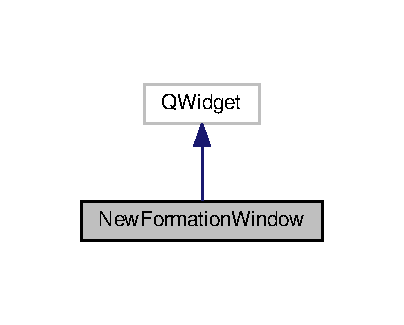
\includegraphics[width=194pt]{class_new_formation_window__inherit__graph}
\end{center}
\end{figure}


Collaboration diagram for New\-Formation\-Window\-:
\nopagebreak
\begin{figure}[H]
\begin{center}
\leavevmode
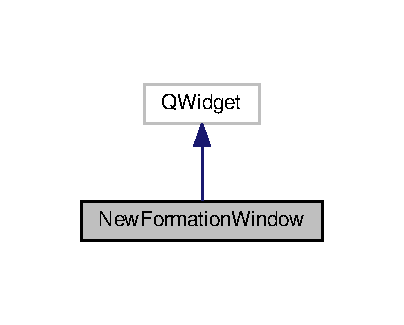
\includegraphics[width=194pt]{class_new_formation_window__coll__graph}
\end{center}
\end{figure}
\subsection*{Public Slots}
\begin{DoxyCompactItemize}
\item 
void \hyperlink{class_new_formation_window_a66635e5ac130cab09c7e356e7f660f28}{setenabled} ()
\begin{DoxyCompactList}\small\item\em Activation du bouton ajouter. \end{DoxyCompactList}\item 
\hypertarget{class_new_formation_window_a8b9f4f31f77835e98c3a07fdaf5fc4fe}{void \hyperlink{class_new_formation_window_a8b9f4f31f77835e98c3a07fdaf5fc4fe}{ajouter} ()}\label{class_new_formation_window_a8b9f4f31f77835e98c3a07fdaf5fc4fe}

\begin{DoxyCompactList}\small\item\em Ajout d'une nouvelle formation dans la table \hyperlink{class_formation}{Formation}. \end{DoxyCompactList}\item 
\hypertarget{class_new_formation_window_aa1bee2b0401c7b3d6717022562eace9c}{void \hyperlink{class_new_formation_window_aa1bee2b0401c7b3d6717022562eace9c}{annuler} ()}\label{class_new_formation_window_aa1bee2b0401c7b3d6717022562eace9c}

\begin{DoxyCompactList}\small\item\em Fermeture de la fenêtre sans ajout de formation. \end{DoxyCompactList}\end{DoxyCompactItemize}
\subsection*{Public Member Functions}
\begin{DoxyCompactItemize}
\item 
\hypertarget{class_new_formation_window_acc9ad7964db8df72b01d628622bc8d24}{\hyperlink{class_new_formation_window_acc9ad7964db8df72b01d628622bc8d24}{New\-Formation\-Window} (\hyperlink{class_formation_window}{Formation\-Window} $\ast$fw)}\label{class_new_formation_window_acc9ad7964db8df72b01d628622bc8d24}

\begin{DoxyCompactList}\small\item\em Constructeur de \hyperlink{class_new_formation_window}{New\-Formation\-Window}. \end{DoxyCompactList}\end{DoxyCompactItemize}
\subsection*{Friends}
\begin{DoxyCompactItemize}
\item 
\hypertarget{class_new_formation_window_a8f86dda6178392bedb6b512d4bf6a6f5}{class {\bfseries Formation\-Window}}\label{class_new_formation_window_a8f86dda6178392bedb6b512d4bf6a6f5}

\end{DoxyCompactItemize}


\subsection{Detailed Description}
Classe qui permet d'ajouter une nouvelle formation. 

Definition at line 1172 of file U\-T\-Profiler.\-h.



\subsection{Member Function Documentation}
\hypertarget{class_new_formation_window_a66635e5ac130cab09c7e356e7f660f28}{\index{New\-Formation\-Window@{New\-Formation\-Window}!setenabled@{setenabled}}
\index{setenabled@{setenabled}!NewFormationWindow@{New\-Formation\-Window}}
\subsubsection[{setenabled}]{\setlength{\rightskip}{0pt plus 5cm}void New\-Formation\-Window\-::setenabled (
\begin{DoxyParamCaption}
{}
\end{DoxyParamCaption}
)\hspace{0.3cm}{\ttfamily [slot]}}}\label{class_new_formation_window_a66635e5ac130cab09c7e356e7f660f28}


Activation du bouton ajouter. 

Active le bouton ajouter lorsque un champ de la fenêtre a été modifié. 

Definition at line 540 of file Formation\-Window.\-cpp.



The documentation for this class was generated from the following files\-:\begin{DoxyCompactItemize}
\item 
\hyperlink{_u_t_profiler_8h}{U\-T\-Profiler.\-h}\item 
\hyperlink{_formation_window_8cpp}{Formation\-Window.\-cpp}\end{DoxyCompactItemize}

\hypertarget{class_new_u_v_window}{\section{New\-U\-V\-Window Class Reference}
\label{class_new_u_v_window}\index{New\-U\-V\-Window@{New\-U\-V\-Window}}
}


Inheritance diagram for New\-U\-V\-Window\-:
\nopagebreak
\begin{figure}[H]
\begin{center}
\leavevmode
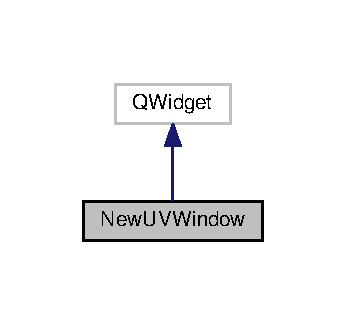
\includegraphics[width=166pt]{class_new_u_v_window__inherit__graph}
\end{center}
\end{figure}


Collaboration diagram for New\-U\-V\-Window\-:
\nopagebreak
\begin{figure}[H]
\begin{center}
\leavevmode
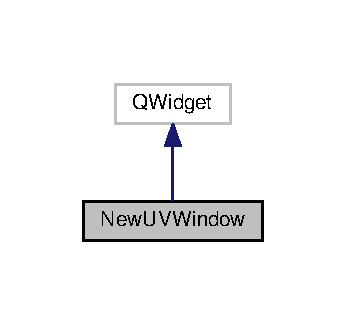
\includegraphics[width=166pt]{class_new_u_v_window__coll__graph}
\end{center}
\end{figure}
\subsection*{Public Slots}
\begin{DoxyCompactItemize}
\item 
\hypertarget{class_new_u_v_window_a13338b8bde9709bfd6b17fe51a201c13}{void {\bfseries pbvalider\-Enable} ()}\label{class_new_u_v_window_a13338b8bde9709bfd6b17fe51a201c13}

\item 
\hypertarget{class_new_u_v_window_a8c423065c475cdf6b9fde1a37e514f48}{void {\bfseries nouveau\-\_\-annuler} ()}\label{class_new_u_v_window_a8c423065c475cdf6b9fde1a37e514f48}

\item 
\hypertarget{class_new_u_v_window_a51046bb303e7f8c19131f4b8d38f8e7c}{void {\bfseries nouveau\-\_\-valider} ()}\label{class_new_u_v_window_a51046bb303e7f8c19131f4b8d38f8e7c}

\end{DoxyCompactItemize}
\subsection*{Friends}
\begin{DoxyCompactItemize}
\item 
\hypertarget{class_new_u_v_window_a33aa3c7d8986c4fe6396f8bf84221386}{class {\bfseries U\-V\-Window}}\label{class_new_u_v_window_a33aa3c7d8986c4fe6396f8bf84221386}

\end{DoxyCompactItemize}


\subsection{Detailed Description}


Definition at line 919 of file U\-T\-Profiler.\-h.



The documentation for this class was generated from the following files\-:\begin{DoxyCompactItemize}
\item 
\hyperlink{_u_t_profiler_8h}{U\-T\-Profiler.\-h}\item 
U\-V\-Window.\-cpp\end{DoxyCompactItemize}

\hypertarget{structqt__meta__stringdata___associer_filiere_window__t}{\section{qt\-\_\-meta\-\_\-stringdata\-\_\-\-Associer\-Filiere\-Window\-\_\-t Struct Reference}
\label{structqt__meta__stringdata___associer_filiere_window__t}\index{qt\-\_\-meta\-\_\-stringdata\-\_\-\-Associer\-Filiere\-Window\-\_\-t@{qt\-\_\-meta\-\_\-stringdata\-\_\-\-Associer\-Filiere\-Window\-\_\-t}}
}
\subsection*{Public Attributes}
\begin{DoxyCompactItemize}
\item 
\hypertarget{structqt__meta__stringdata___associer_filiere_window__t_aebfac119d9c30de5c8bf598a450c7a48}{Q\-Byte\-Array\-Data {\bfseries data} \mbox{[}3\mbox{]}}\label{structqt__meta__stringdata___associer_filiere_window__t_aebfac119d9c30de5c8bf598a450c7a48}

\item 
\hypertarget{structqt__meta__stringdata___associer_filiere_window__t_a26f17e8c3d42905adf900756edcb0e2e}{char {\bfseries stringdata} \mbox{[}32\mbox{]}}\label{structqt__meta__stringdata___associer_filiere_window__t_a26f17e8c3d42905adf900756edcb0e2e}

\end{DoxyCompactItemize}


\subsection{Detailed Description}


Definition at line 1228 of file moc\-\_\-\-U\-T\-Profiler.\-cpp.



The documentation for this struct was generated from the following file\-:\begin{DoxyCompactItemize}
\item 
/home/timothee/\-Documents/\-L\-O21/\-U\-T\-Profiler/build-\/\-U\-T\-Profiler-\/\-Desktop-\/\-Debug/moc\-\_\-\-U\-T\-Profiler.\-cpp\end{DoxyCompactItemize}

\hypertarget{structqt__meta__stringdata___associer_u_v_window__t}{\section{qt\-\_\-meta\-\_\-stringdata\-\_\-\-Associer\-U\-V\-Window\-\_\-t Struct Reference}
\label{structqt__meta__stringdata___associer_u_v_window__t}\index{qt\-\_\-meta\-\_\-stringdata\-\_\-\-Associer\-U\-V\-Window\-\_\-t@{qt\-\_\-meta\-\_\-stringdata\-\_\-\-Associer\-U\-V\-Window\-\_\-t}}
}
\subsection*{Public Attributes}
\begin{DoxyCompactItemize}
\item 
\hypertarget{structqt__meta__stringdata___associer_u_v_window__t_adca27a5b25bcca9aad8a23c5d2f706a4}{Q\-Byte\-Array\-Data {\bfseries data} \mbox{[}3\mbox{]}}\label{structqt__meta__stringdata___associer_u_v_window__t_adca27a5b25bcca9aad8a23c5d2f706a4}

\item 
\hypertarget{structqt__meta__stringdata___associer_u_v_window__t_acb0d547f52eb5781c45566800e53f5aa}{char {\bfseries stringdata} \mbox{[}27\mbox{]}}\label{structqt__meta__stringdata___associer_u_v_window__t_acb0d547f52eb5781c45566800e53f5aa}

\end{DoxyCompactItemize}


\subsection{Detailed Description}


Definition at line 1140 of file moc\-\_\-\-U\-T\-Profiler.\-cpp.



The documentation for this struct was generated from the following file\-:\begin{DoxyCompactItemize}
\item 
/home/timothee/\-Documents/\-L\-O21/\-U\-T\-Profiler/build-\/\-U\-T\-Profiler-\/\-Desktop-\/\-Debug/moc\-\_\-\-U\-T\-Profiler.\-cpp\end{DoxyCompactItemize}

\hypertarget{structqt__meta__stringdata___completion_profil_window__t}{\section{qt\-\_\-meta\-\_\-stringdata\-\_\-\-Completion\-Profil\-Window\-\_\-t Struct Reference}
\label{structqt__meta__stringdata___completion_profil_window__t}\index{qt\-\_\-meta\-\_\-stringdata\-\_\-\-Completion\-Profil\-Window\-\_\-t@{qt\-\_\-meta\-\_\-stringdata\-\_\-\-Completion\-Profil\-Window\-\_\-t}}
}
\subsection*{Public Attributes}
\begin{DoxyCompactItemize}
\item 
\hypertarget{structqt__meta__stringdata___completion_profil_window__t_af7077185398b681ff57b1906f979b24a}{Q\-Byte\-Array\-Data {\bfseries data} \mbox{[}16\mbox{]}}\label{structqt__meta__stringdata___completion_profil_window__t_af7077185398b681ff57b1906f979b24a}

\item 
\hypertarget{structqt__meta__stringdata___completion_profil_window__t_a943885b68fdb9fc1a159a4aab0706282}{char {\bfseries stringdata} \mbox{[}168\mbox{]}}\label{structqt__meta__stringdata___completion_profil_window__t_a943885b68fdb9fc1a159a4aab0706282}

\end{DoxyCompactItemize}


\subsection{Detailed Description}


Definition at line 929 of file moc\-\_\-\-U\-T\-Profiler.\-cpp.



The documentation for this struct was generated from the following file\-:\begin{DoxyCompactItemize}
\item 
/home/timothee/\-Documents/\-L\-O21/\-U\-T\-Profiler/build-\/\-U\-T\-Profiler-\/\-Desktop-\/\-Debug/moc\-\_\-\-U\-T\-Profiler.\-cpp\end{DoxyCompactItemize}

\hypertarget{structqt__meta__stringdata___dossier_window__t}{\section{qt\-\_\-meta\-\_\-stringdata\-\_\-\-Dossier\-Window\-\_\-t Struct Reference}
\label{structqt__meta__stringdata___dossier_window__t}\index{qt\-\_\-meta\-\_\-stringdata\-\_\-\-Dossier\-Window\-\_\-t@{qt\-\_\-meta\-\_\-stringdata\-\_\-\-Dossier\-Window\-\_\-t}}
}
\subsection*{Public Attributes}
\begin{DoxyCompactItemize}
\item 
\hypertarget{structqt__meta__stringdata___dossier_window__t_a03913a64e3eba6ca43b00dc26d65b925}{Q\-Byte\-Array\-Data {\bfseries data} \mbox{[}12\mbox{]}}\label{structqt__meta__stringdata___dossier_window__t_a03913a64e3eba6ca43b00dc26d65b925}

\item 
\hypertarget{structqt__meta__stringdata___dossier_window__t_af4a224001829112f4e5614deb18c5274}{char {\bfseries stringdata} \mbox{[}121\mbox{]}}\label{structqt__meta__stringdata___dossier_window__t_af4a224001829112f4e5614deb18c5274}

\end{DoxyCompactItemize}


\subsection{Detailed Description}


Definition at line 223 of file moc\-\_\-\-U\-T\-Profiler.\-cpp.



The documentation for this struct was generated from the following file\-:\begin{DoxyCompactItemize}
\item 
/home/timothee/\-Documents/\-L\-O21/\-U\-T\-Profiler/build-\/\-U\-T\-Profiler-\/\-Desktop-\/\-Debug/moc\-\_\-\-U\-T\-Profiler.\-cpp\end{DoxyCompactItemize}

\hypertarget{structqt__meta__stringdata___formation_ext_window__t}{\section{qt\-\_\-meta\-\_\-stringdata\-\_\-\-Formation\-Ext\-Window\-\_\-t Struct Reference}
\label{structqt__meta__stringdata___formation_ext_window__t}\index{qt\-\_\-meta\-\_\-stringdata\-\_\-\-Formation\-Ext\-Window\-\_\-t@{qt\-\_\-meta\-\_\-stringdata\-\_\-\-Formation\-Ext\-Window\-\_\-t}}
}
\subsection*{Public Attributes}
\begin{DoxyCompactItemize}
\item 
\hypertarget{structqt__meta__stringdata___formation_ext_window__t_a0b77957c957a98850a2f9ad9d1cee1ab}{Q\-Byte\-Array\-Data {\bfseries data} \mbox{[}3\mbox{]}}\label{structqt__meta__stringdata___formation_ext_window__t_a0b77957c957a98850a2f9ad9d1cee1ab}

\item 
\hypertarget{structqt__meta__stringdata___formation_ext_window__t_ad90fbbe95508e5217246237f1d0d81c9}{char {\bfseries stringdata} \mbox{[}29\mbox{]}}\label{structqt__meta__stringdata___formation_ext_window__t_ad90fbbe95508e5217246237f1d0d81c9}

\end{DoxyCompactItemize}


\subsection{Detailed Description}


Definition at line 343 of file moc\-\_\-\-U\-T\-Profiler.\-cpp.



The documentation for this struct was generated from the following file\-:\begin{DoxyCompactItemize}
\item 
/home/timothee/\-Documents/\-L\-O21/\-U\-T\-Profiler/build-\/\-U\-T\-Profiler-\/\-Desktop-\/\-Debug/moc\-\_\-\-U\-T\-Profiler.\-cpp\end{DoxyCompactItemize}

\hypertarget{structqt__meta__stringdata___formation_window__t}{\section{qt\-\_\-meta\-\_\-stringdata\-\_\-\-Formation\-Window\-\_\-t Struct Reference}
\label{structqt__meta__stringdata___formation_window__t}\index{qt\-\_\-meta\-\_\-stringdata\-\_\-\-Formation\-Window\-\_\-t@{qt\-\_\-meta\-\_\-stringdata\-\_\-\-Formation\-Window\-\_\-t}}
}
\subsection*{Public Attributes}
\begin{DoxyCompactItemize}
\item 
\hypertarget{structqt__meta__stringdata___formation_window__t_a416d542b4210f16927582f25e93d835b}{Q\-Byte\-Array\-Data {\bfseries data} \mbox{[}13\mbox{]}}\label{structqt__meta__stringdata___formation_window__t_a416d542b4210f16927582f25e93d835b}

\item 
\hypertarget{structqt__meta__stringdata___formation_window__t_a77e6f6fc0cc270b369d4fe6beb7823df}{char {\bfseries stringdata} \mbox{[}109\mbox{]}}\label{structqt__meta__stringdata___formation_window__t_a77e6f6fc0cc270b369d4fe6beb7823df}

\end{DoxyCompactItemize}


\subsection{Detailed Description}


Definition at line 616 of file moc\-\_\-\-U\-T\-Profiler.\-cpp.



The documentation for this struct was generated from the following file\-:\begin{DoxyCompactItemize}
\item 
/home/timothee/\-Documents/\-L\-O21/\-U\-T\-Profiler/build-\/\-U\-T\-Profiler-\/\-Desktop-\/\-Debug/moc\-\_\-\-U\-T\-Profiler.\-cpp\end{DoxyCompactItemize}

\hypertarget{structqt__meta__stringdata___home_window__t}{\section{qt\-\_\-meta\-\_\-stringdata\-\_\-\-Home\-Window\-\_\-t Struct Reference}
\label{structqt__meta__stringdata___home_window__t}\index{qt\-\_\-meta\-\_\-stringdata\-\_\-\-Home\-Window\-\_\-t@{qt\-\_\-meta\-\_\-stringdata\-\_\-\-Home\-Window\-\_\-t}}
}
\subsection*{Public Attributes}
\begin{DoxyCompactItemize}
\item 
\hypertarget{structqt__meta__stringdata___home_window__t_a64121fd145bf51f5500e6a1903bb8ee2}{Q\-Byte\-Array\-Data {\bfseries data} \mbox{[}1\mbox{]}}\label{structqt__meta__stringdata___home_window__t_a64121fd145bf51f5500e6a1903bb8ee2}

\item 
\hypertarget{structqt__meta__stringdata___home_window__t_af51d1c571fa38cf04ac3be1bc2067171}{char {\bfseries stringdata} \mbox{[}12\mbox{]}}\label{structqt__meta__stringdata___home_window__t_af51d1c571fa38cf04ac3be1bc2067171}

\end{DoxyCompactItemize}


\subsection{Detailed Description}


Definition at line 1073 of file moc\-\_\-\-U\-T\-Profiler.\-cpp.



The documentation for this struct was generated from the following file\-:\begin{DoxyCompactItemize}
\item 
/home/timothee/\-Documents/\-L\-O21/\-U\-T\-Profiler/build-\/\-U\-T\-Profiler-\/\-Desktop-\/\-Debug/moc\-\_\-\-U\-T\-Profiler.\-cpp\end{DoxyCompactItemize}

\hypertarget{structqt__meta__stringdata___new_formation_window__t}{\section{qt\-\_\-meta\-\_\-stringdata\-\_\-\-New\-Formation\-Window\-\_\-t Struct Reference}
\label{structqt__meta__stringdata___new_formation_window__t}\index{qt\-\_\-meta\-\_\-stringdata\-\_\-\-New\-Formation\-Window\-\_\-t@{qt\-\_\-meta\-\_\-stringdata\-\_\-\-New\-Formation\-Window\-\_\-t}}
}
\subsection*{Public Attributes}
\begin{DoxyCompactItemize}
\item 
\hypertarget{structqt__meta__stringdata___new_formation_window__t_a1adc4e8ad5abaf0be36e061a70fbeef7}{Q\-Byte\-Array\-Data {\bfseries data} \mbox{[}5\mbox{]}}\label{structqt__meta__stringdata___new_formation_window__t_a1adc4e8ad5abaf0be36e061a70fbeef7}

\item 
\hypertarget{structqt__meta__stringdata___new_formation_window__t_ac8539fb19c68ebd04d854752aeb4fd81}{char {\bfseries stringdata} \mbox{[}48\mbox{]}}\label{structqt__meta__stringdata___new_formation_window__t_ac8539fb19c68ebd04d854752aeb4fd81}

\end{DoxyCompactItemize}


\subsection{Detailed Description}


Definition at line 519 of file moc\-\_\-\-U\-T\-Profiler.\-cpp.



The documentation for this struct was generated from the following file\-:\begin{DoxyCompactItemize}
\item 
/home/timothee/\-Documents/\-L\-O21/\-U\-T\-Profiler/build-\/\-U\-T\-Profiler-\/\-Desktop-\/\-Debug/moc\-\_\-\-U\-T\-Profiler.\-cpp\end{DoxyCompactItemize}

\hypertarget{structqt__meta__stringdata___new_u_v_window__t}{\section{qt\-\_\-meta\-\_\-stringdata\-\_\-\-New\-U\-V\-Window\-\_\-t Struct Reference}
\label{structqt__meta__stringdata___new_u_v_window__t}\index{qt\-\_\-meta\-\_\-stringdata\-\_\-\-New\-U\-V\-Window\-\_\-t@{qt\-\_\-meta\-\_\-stringdata\-\_\-\-New\-U\-V\-Window\-\_\-t}}
}
\subsection*{Public Attributes}
\begin{DoxyCompactItemize}
\item 
\hypertarget{structqt__meta__stringdata___new_u_v_window__t_a07a2059bda726b169e79aae235bdfe4f}{Q\-Byte\-Array\-Data {\bfseries data} \mbox{[}5\mbox{]}}\label{structqt__meta__stringdata___new_u_v_window__t_a07a2059bda726b169e79aae235bdfe4f}

\item 
\hypertarget{structqt__meta__stringdata___new_u_v_window__t_ae2c41912179cb2fa30419e9a743aefd5}{char {\bfseries stringdata} \mbox{[}62\mbox{]}}\label{structqt__meta__stringdata___new_u_v_window__t_ae2c41912179cb2fa30419e9a743aefd5}

\end{DoxyCompactItemize}


\subsection{Detailed Description}


Definition at line 21 of file moc\-\_\-\-U\-T\-Profiler.\-cpp.



The documentation for this struct was generated from the following file\-:\begin{DoxyCompactItemize}
\item 
/home/timothee/\-Documents/\-L\-O21/\-U\-T\-Profiler/build-\/\-U\-T\-Profiler-\/\-Desktop-\/\-Debug/moc\-\_\-\-U\-T\-Profiler.\-cpp\end{DoxyCompactItemize}

\hypertarget{structqt__meta__stringdata___retrouver_completion_window__t}{\section{qt\-\_\-meta\-\_\-stringdata\-\_\-\-Retrouver\-Completion\-Window\-\_\-t Struct Reference}
\label{structqt__meta__stringdata___retrouver_completion_window__t}\index{qt\-\_\-meta\-\_\-stringdata\-\_\-\-Retrouver\-Completion\-Window\-\_\-t@{qt\-\_\-meta\-\_\-stringdata\-\_\-\-Retrouver\-Completion\-Window\-\_\-t}}
}
\subsection*{Public Attributes}
\begin{DoxyCompactItemize}
\item 
\hypertarget{structqt__meta__stringdata___retrouver_completion_window__t_aea3d59f7bb53c9c2fccd944d0741d466}{Q\-Byte\-Array\-Data {\bfseries data} \mbox{[}4\mbox{]}}\label{structqt__meta__stringdata___retrouver_completion_window__t_aea3d59f7bb53c9c2fccd944d0741d466}

\item 
\hypertarget{structqt__meta__stringdata___retrouver_completion_window__t_a0ec59f2b31c3c86fe5a226768b092f34}{char {\bfseries stringdata} \mbox{[}46\mbox{]}}\label{structqt__meta__stringdata___retrouver_completion_window__t_a0ec59f2b31c3c86fe5a226768b092f34}

\end{DoxyCompactItemize}


\subsection{Detailed Description}


Definition at line 836 of file moc\-\_\-\-U\-T\-Profiler.\-cpp.



The documentation for this struct was generated from the following file\-:\begin{DoxyCompactItemize}
\item 
/home/timothee/\-Documents/\-L\-O21/\-U\-T\-Profiler/build-\/\-U\-T\-Profiler-\/\-Desktop-\/\-Debug/moc\-\_\-\-U\-T\-Profiler.\-cpp\end{DoxyCompactItemize}

\hypertarget{structqt__meta__stringdata___search_dossier_window__t}{\section{qt\-\_\-meta\-\_\-stringdata\-\_\-\-Search\-Dossier\-Window\-\_\-t Struct Reference}
\label{structqt__meta__stringdata___search_dossier_window__t}\index{qt\-\_\-meta\-\_\-stringdata\-\_\-\-Search\-Dossier\-Window\-\_\-t@{qt\-\_\-meta\-\_\-stringdata\-\_\-\-Search\-Dossier\-Window\-\_\-t}}
}
\subsection*{Public Attributes}
\begin{DoxyCompactItemize}
\item 
\hypertarget{structqt__meta__stringdata___search_dossier_window__t_ac9d2789437eef387995aaad096d92f17}{Q\-Byte\-Array\-Data {\bfseries data} \mbox{[}5\mbox{]}}\label{structqt__meta__stringdata___search_dossier_window__t_ac9d2789437eef387995aaad096d92f17}

\item 
\hypertarget{structqt__meta__stringdata___search_dossier_window__t_aa2489fbe3f2fcbe10c9a0e076c09c972}{char {\bfseries stringdata} \mbox{[}51\mbox{]}}\label{structqt__meta__stringdata___search_dossier_window__t_aa2489fbe3f2fcbe10c9a0e076c09c972}

\end{DoxyCompactItemize}


\subsection{Detailed Description}


Definition at line 739 of file moc\-\_\-\-U\-T\-Profiler.\-cpp.



The documentation for this struct was generated from the following file\-:\begin{DoxyCompactItemize}
\item 
/home/timothee/\-Documents/\-L\-O21/\-U\-T\-Profiler/build-\/\-U\-T\-Profiler-\/\-Desktop-\/\-Debug/moc\-\_\-\-U\-T\-Profiler.\-cpp\end{DoxyCompactItemize}

\hypertarget{structqt__meta__stringdata___semestre_window__t}{\section{qt\-\_\-meta\-\_\-stringdata\-\_\-\-Semestre\-Window\-\_\-t Struct Reference}
\label{structqt__meta__stringdata___semestre_window__t}\index{qt\-\_\-meta\-\_\-stringdata\-\_\-\-Semestre\-Window\-\_\-t@{qt\-\_\-meta\-\_\-stringdata\-\_\-\-Semestre\-Window\-\_\-t}}
}
\subsection*{Public Attributes}
\begin{DoxyCompactItemize}
\item 
\hypertarget{structqt__meta__stringdata___semestre_window__t_a705061d9dcb53d8e0d13e22f7b088c5e}{Q\-Byte\-Array\-Data {\bfseries data} \mbox{[}3\mbox{]}}\label{structqt__meta__stringdata___semestre_window__t_a705061d9dcb53d8e0d13e22f7b088c5e}

\item 
\hypertarget{structqt__meta__stringdata___semestre_window__t_ab7624d0549fca6d65ba502cb2790e27c}{char {\bfseries stringdata} \mbox{[}25\mbox{]}}\label{structqt__meta__stringdata___semestre_window__t_ab7624d0549fca6d65ba502cb2790e27c}

\end{DoxyCompactItemize}


\subsection{Detailed Description}


Definition at line 431 of file moc\-\_\-\-U\-T\-Profiler.\-cpp.



The documentation for this struct was generated from the following file\-:\begin{DoxyCompactItemize}
\item 
/home/timothee/\-Documents/\-L\-O21/\-U\-T\-Profiler/build-\/\-U\-T\-Profiler-\/\-Desktop-\/\-Debug/moc\-\_\-\-U\-T\-Profiler.\-cpp\end{DoxyCompactItemize}

\hypertarget{structqt__meta__stringdata___u_v_window__t}{\section{qt\-\_\-meta\-\_\-stringdata\-\_\-\-U\-V\-Window\-\_\-t Struct Reference}
\label{structqt__meta__stringdata___u_v_window__t}\index{qt\-\_\-meta\-\_\-stringdata\-\_\-\-U\-V\-Window\-\_\-t@{qt\-\_\-meta\-\_\-stringdata\-\_\-\-U\-V\-Window\-\_\-t}}
}
\subsection*{Public Attributes}
\begin{DoxyCompactItemize}
\item 
\hypertarget{structqt__meta__stringdata___u_v_window__t_a8d6f241a1a98c720b3ec974889a66bb7}{Q\-Byte\-Array\-Data {\bfseries data} \mbox{[}7\mbox{]}}\label{structqt__meta__stringdata___u_v_window__t_a8d6f241a1a98c720b3ec974889a66bb7}

\item 
\hypertarget{structqt__meta__stringdata___u_v_window__t_aea165668963a3225679b8f30692af0ba}{char {\bfseries stringdata} \mbox{[}62\mbox{]}}\label{structqt__meta__stringdata___u_v_window__t_aea165668963a3225679b8f30692af0ba}

\end{DoxyCompactItemize}


\subsection{Detailed Description}


Definition at line 118 of file moc\-\_\-\-U\-T\-Profiler.\-cpp.



The documentation for this struct was generated from the following file\-:\begin{DoxyCompactItemize}
\item 
/home/timothee/\-Documents/\-L\-O21/\-U\-T\-Profiler/build-\/\-U\-T\-Profiler-\/\-Desktop-\/\-Debug/moc\-\_\-\-U\-T\-Profiler.\-cpp\end{DoxyCompactItemize}

\hypertarget{class_retrouver_completion_window}{\section{Retrouver\-Completion\-Window Class Reference}
\label{class_retrouver_completion_window}\index{Retrouver\-Completion\-Window@{Retrouver\-Completion\-Window}}
}


Inheritance diagram for Retrouver\-Completion\-Window\-:
\nopagebreak
\begin{figure}[H]
\begin{center}
\leavevmode
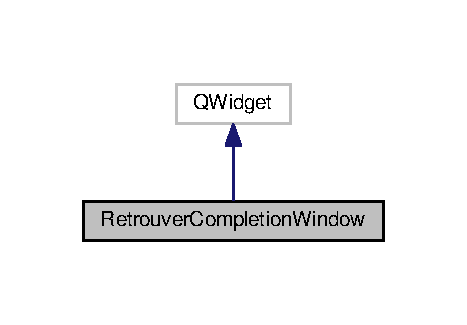
\includegraphics[width=224pt]{class_retrouver_completion_window__inherit__graph}
\end{center}
\end{figure}


Collaboration diagram for Retrouver\-Completion\-Window\-:
\nopagebreak
\begin{figure}[H]
\begin{center}
\leavevmode
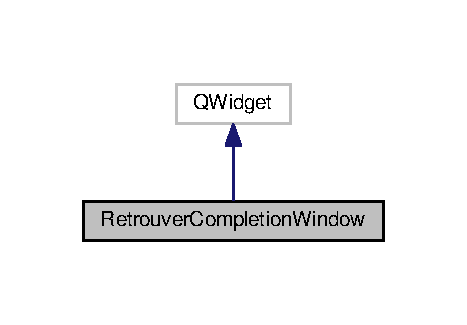
\includegraphics[width=224pt]{class_retrouver_completion_window__coll__graph}
\end{center}
\end{figure}
\subsection*{Public Slots}
\begin{DoxyCompactItemize}
\item 
\hypertarget{class_retrouver_completion_window_a29cbfc2c4c6008dd4975395cfb9cc97a}{void \hyperlink{class_retrouver_completion_window_a29cbfc2c4c6008dd4975395cfb9cc97a}{precedent} ()}\label{class_retrouver_completion_window_a29cbfc2c4c6008dd4975395cfb9cc97a}

\begin{DoxyCompactList}\small\item\em Retrouver. \end{DoxyCompactList}\item 
\hypertarget{class_retrouver_completion_window_a44b071eea4a996a30d5f7ad9ea345dc5}{void {\bfseries suivant} ()}\label{class_retrouver_completion_window_a44b071eea4a996a30d5f7ad9ea345dc5}

\end{DoxyCompactItemize}
\subsection*{Public Member Functions}
\begin{DoxyCompactItemize}
\item 
\hyperlink{class_retrouver_completion_window_ac8977a4ac244917a090cd77f59712abe}{Retrouver\-Completion\-Window} (Q\-String $\ast$$\ast$$\ast$c)
\begin{DoxyCompactList}\small\item\em Constructeur Ce constructeur initialise toutes les fonctions de l'Interface Graphique de cette fenêtre \-: créer et organiser les objets graphiques, et les connecter avec les bons slots. De plus, il remplit automatiquement les champs grâce au tableau passé en paramètre. \end{DoxyCompactList}\item 
\hypertarget{class_retrouver_completion_window_ab7a253bbab907827888e4cf32af54330}{void {\bfseries associercompletion} (Q\-String $\ast$$\ast$completion)}\label{class_retrouver_completion_window_ab7a253bbab907827888e4cf32af54330}

\end{DoxyCompactItemize}
\subsection*{Friends}
\begin{DoxyCompactItemize}
\item 
\hypertarget{class_retrouver_completion_window_a4a44bd2bee11aa6e41709ed1a35a875d}{class {\bfseries Search\-Dossier\-Window}}\label{class_retrouver_completion_window_a4a44bd2bee11aa6e41709ed1a35a875d}

\end{DoxyCompactItemize}


\subsection{Detailed Description}


Definition at line 1291 of file U\-T\-Profiler.\-h.



\subsection{Constructor \& Destructor Documentation}
\hypertarget{class_retrouver_completion_window_ac8977a4ac244917a090cd77f59712abe}{\index{Retrouver\-Completion\-Window@{Retrouver\-Completion\-Window}!Retrouver\-Completion\-Window@{Retrouver\-Completion\-Window}}
\index{Retrouver\-Completion\-Window@{Retrouver\-Completion\-Window}!RetrouverCompletionWindow@{Retrouver\-Completion\-Window}}
\subsubsection[{Retrouver\-Completion\-Window}]{\setlength{\rightskip}{0pt plus 5cm}Retrouver\-Completion\-Window\-::\-Retrouver\-Completion\-Window (
\begin{DoxyParamCaption}
\item[{Q\-String $\ast$$\ast$$\ast$}]{c}
\end{DoxyParamCaption}
)}}\label{class_retrouver_completion_window_ac8977a4ac244917a090cd77f59712abe}


Constructeur Ce constructeur initialise toutes les fonctions de l'Interface Graphique de cette fenêtre \-: créer et organiser les objets graphiques, et les connecter avec les bons slots. De plus, il remplit automatiquement les champs grâce au tableau passé en paramètre. 


\begin{DoxyParams}{Parameters}
{\em c} & \-: tableau des différentes complétions enregistrées \\
\hline
\end{DoxyParams}


Definition at line 445 of file Completion\-Profil\-Window.\-cpp.



The documentation for this class was generated from the following files\-:\begin{DoxyCompactItemize}
\item 
\hyperlink{_u_t_profiler_8h}{U\-T\-Profiler.\-h}\item 
Completion\-Profil\-Window.\-cpp\end{DoxyCompactItemize}

\hypertarget{class_search_dossier_window}{\section{Search\-Dossier\-Window Class Reference}
\label{class_search_dossier_window}\index{Search\-Dossier\-Window@{Search\-Dossier\-Window}}
}


Inheritance diagram for Search\-Dossier\-Window\-:
\nopagebreak
\begin{figure}[H]
\begin{center}
\leavevmode
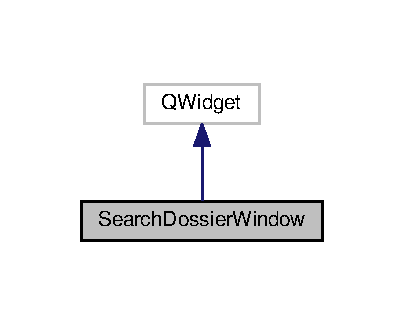
\includegraphics[width=194pt]{class_search_dossier_window__inherit__graph}
\end{center}
\end{figure}


Collaboration diagram for Search\-Dossier\-Window\-:
\nopagebreak
\begin{figure}[H]
\begin{center}
\leavevmode
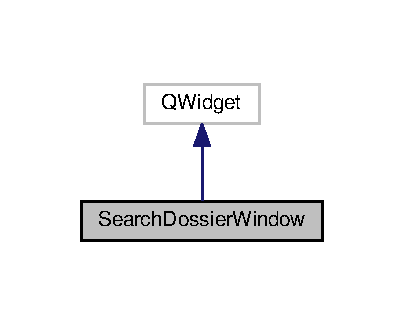
\includegraphics[width=194pt]{class_search_dossier_window__coll__graph}
\end{center}
\end{figure}
\subsection*{Public Slots}
\begin{DoxyCompactItemize}
\item 
\hypertarget{class_search_dossier_window_a15f74a894eef1feeab8265b025cfc020}{void \hyperlink{class_search_dossier_window_a15f74a894eef1feeab8265b025cfc020}{rechercher} ()}\label{class_search_dossier_window_a15f74a894eef1feeab8265b025cfc020}

\begin{DoxyCompactList}\small\item\em Slot permettant de rechercher un dossier dans la base de données. \end{DoxyCompactList}\item 
\hypertarget{class_search_dossier_window_ae289e7718b2b726e7b1c42bfa87ca836}{void \hyperlink{class_search_dossier_window_ae289e7718b2b726e7b1c42bfa87ca836}{retrouver} ()}\label{class_search_dossier_window_ae289e7718b2b726e7b1c42bfa87ca836}

\begin{DoxyCompactList}\small\item\em Slot permettant d'ouvrir la fenêtre de consultation des completions de profil enrigistrées après avoir séléctionné un dossier. \end{DoxyCompactList}\item 
\hypertarget{class_search_dossier_window_a59fb8abcad92a95d6b7d3d8319abe68e}{void \hyperlink{class_search_dossier_window_a59fb8abcad92a95d6b7d3d8319abe68e}{annuler} ()}\label{class_search_dossier_window_a59fb8abcad92a95d6b7d3d8319abe68e}

\begin{DoxyCompactList}\small\item\em Slot permettant de revenir à l'écran précédent. \end{DoxyCompactList}\end{DoxyCompactItemize}
\subsection*{Public Member Functions}
\begin{DoxyCompactItemize}
\item 
\hyperlink{class_search_dossier_window_a9471fbc6309afca4c7b7a3bb68a907d7}{Search\-Dossier\-Window} (\hyperlink{class_completion_profil_window}{Completion\-Profil\-Window} $\ast$fw)
\begin{DoxyCompactList}\small\item\em Constructeur Ce constructeur initialise toutes les fonctions de l'Interface Graphique de cette fenêtre \-: créer et organiser les objets graphiques, et les connecter avec les bons slots. \end{DoxyCompactList}\end{DoxyCompactItemize}
\subsection*{Friends}
\begin{DoxyCompactItemize}
\item 
\hypertarget{class_search_dossier_window_a28011ad12f1da757a3c035c4be934793}{class {\bfseries Completion\-Profil\-Window}}\label{class_search_dossier_window_a28011ad12f1da757a3c035c4be934793}

\item 
\hypertarget{class_search_dossier_window_a89f0e38a39f054c26a0ab852f8a79b18}{class {\bfseries Home\-Window}}\label{class_search_dossier_window_a89f0e38a39f054c26a0ab852f8a79b18}

\end{DoxyCompactItemize}


\subsection{Detailed Description}


Definition at line 1260 of file U\-T\-Profiler.\-h.



\subsection{Constructor \& Destructor Documentation}
\hypertarget{class_search_dossier_window_a9471fbc6309afca4c7b7a3bb68a907d7}{\index{Search\-Dossier\-Window@{Search\-Dossier\-Window}!Search\-Dossier\-Window@{Search\-Dossier\-Window}}
\index{Search\-Dossier\-Window@{Search\-Dossier\-Window}!SearchDossierWindow@{Search\-Dossier\-Window}}
\subsubsection[{Search\-Dossier\-Window}]{\setlength{\rightskip}{0pt plus 5cm}Search\-Dossier\-Window\-::\-Search\-Dossier\-Window (
\begin{DoxyParamCaption}
\item[{{\bf Completion\-Profil\-Window} $\ast$}]{fw}
\end{DoxyParamCaption}
)}}\label{class_search_dossier_window_a9471fbc6309afca4c7b7a3bb68a907d7}


Constructeur Ce constructeur initialise toutes les fonctions de l'Interface Graphique de cette fenêtre \-: créer et organiser les objets graphiques, et les connecter avec les bons slots. 


\begin{DoxyParams}{Parameters}
{\em fw} & \-: pointeur vers la classe \hyperlink{class_completion_profil_window}{Completion\-Profil\-Window} qui gère son cycle de vie \\
\hline
\end{DoxyParams}


Definition at line 194 of file Completion\-Profil\-Window.\-cpp.



The documentation for this class was generated from the following files\-:\begin{DoxyCompactItemize}
\item 
\hyperlink{_u_t_profiler_8h}{U\-T\-Profiler.\-h}\item 
Completion\-Profil\-Window.\-cpp\end{DoxyCompactItemize}

\hypertarget{class_semestre}{\section{Semestre Class Reference}
\label{class_semestre}\index{Semestre@{Semestre}}
}


Classe permettant de décrire un semestre d'un étudiant de l'U\-T\-C.  




{\ttfamily \#include $<$U\-T\-Profiler.\-h$>$}

\subsection*{Public Member Functions}
\begin{DoxyCompactItemize}
\item 
\hyperlink{class_semestre_a3980fc8447360ad2ba3c769e40ed0efa}{Semestre} (unsigned int a, \hyperlink{_u_t_profiler_8h_a72fcaae0ef529616dd62b747e259d545}{Saison} s, string c=\char`\"{}\char`\"{})
\begin{DoxyCompactList}\small\item\em Constructeur Permet de créer un objet \hyperlink{class_semestre}{Semestre} initialisé avec les valeurs passées en paramètres. \end{DoxyCompactList}\item 
\hypertarget{class_semestre_a5a495cd21f249b5a1be4d3c7ebd01e88}{\hyperlink{class_semestre_a5a495cd21f249b5a1be4d3c7ebd01e88}{$\sim$\-Semestre} ()}\label{class_semestre_a5a495cd21f249b5a1be4d3c7ebd01e88}

\begin{DoxyCompactList}\small\item\em Destructeur. \end{DoxyCompactList}\item 
unsigned int \hyperlink{class_semestre_a5aa85395e97f58f491ebf251da8231ef}{get\-Annee} () const 
\begin{DoxyCompactList}\small\item\em Accesseur en lecture de l'année en cours au moment du semestre. \end{DoxyCompactList}\item 
\hyperlink{_u_t_profiler_8h_a72fcaae0ef529616dd62b747e259d545}{Saison} \hyperlink{class_semestre_a26e25575e7fb65649c47970a9800c3aa}{get\-Saison} () const 
\begin{DoxyCompactList}\small\item\em Accesseur en lecture de la saison en cours au moment du semestre. \end{DoxyCompactList}\item 
string \hyperlink{class_semestre_aa6f8274d5868ee938767865bb8e66c25}{get\-Commentaire} () const 
\begin{DoxyCompactList}\small\item\em Accesseur en lecture du commentaire du jury quant aux résultats de l'étudiant ce semestre. \end{DoxyCompactList}\item 
\hyperlink{class_inscription}{Inscription} $\ast$ \hyperlink{class_semestre_ac1724b1d1c28eb943496004b44645365}{get\-Inscriptions} () const 
\begin{DoxyCompactList}\small\item\em Accesseur en lecture du tableau des inscritptions aux U\-Vs de l'étudiant ce semestre. \end{DoxyCompactList}\item 
bool \hyperlink{class_semestre_aac6af5aa5fc34383afc56a68862329e2}{get\-Ext} () const 
\begin{DoxyCompactList}\small\item\em Accesseur en lecture du booléen décrivant si l'étudiant était ou non en formation extérieure durant ce semestre. \end{DoxyCompactList}\item 
\hyperlink{class_formation_exterieure}{Formation\-Exterieure} $\ast$ \hyperlink{class_semestre_afeafdde29055295918dc26b31d1980a0}{get\-Formation\-Exterieure} () const 
\begin{DoxyCompactList}\small\item\em Accesseur en lecture du pointeur vers la formation extérieure suivie par l'étudiant ce semestre, s'il en a suivi une. \end{DoxyCompactList}\item 
void \hyperlink{class_semestre_a7d59af6d380e9c204638fa45bdadae0d}{set\-Annee} (unsigned int i)
\begin{DoxyCompactList}\small\item\em Accesseur en écriture de l'année au moment du semestre. \end{DoxyCompactList}\item 
void \hyperlink{class_semestre_aae3da84ef2e291dca3360330ff0ec990}{set\-Saison} (\hyperlink{_u_t_profiler_8h_a72fcaae0ef529616dd62b747e259d545}{Saison} \&s)
\begin{DoxyCompactList}\small\item\em Accesseur en écriture de la saison (Printemps ou Automne) au moment du semestre. \end{DoxyCompactList}\item 
void \hyperlink{class_semestre_a6120eb48d6cd7363c405332ba5a46d75}{set\-Commentaire} (const string \&s)
\begin{DoxyCompactList}\small\item\em Accesseur en écriture du commentaire du jury quant à la réussite de l'étudiant ce semestre. \end{DoxyCompactList}\item 
void \hyperlink{class_semestre_aa77efecd8daa99ab76cb7acf0e868470}{set\-Inscriptions} (\hyperlink{class_inscription}{Inscription} $\ast$i)
\begin{DoxyCompactList}\small\item\em Accesseur en écriture du tableau d'inscriptions aux U\-Vs de l'étudiant ce semestre. \end{DoxyCompactList}\item 
void \hyperlink{class_semestre_a673fc1c0bf3a9dbaeb784d603ac58eb4}{set\-Ext} (bool e)
\begin{DoxyCompactList}\small\item\em Accesseur en écriture du booléen décrivant si l'étudiant suivait ou non une formation exterieure ce semestre. \end{DoxyCompactList}\item 
void \hyperlink{class_semestre_ad263768ddd1fbb8756340e5593241c75}{set\-Formation\-Exterieure} (\hyperlink{class_formation_exterieure}{Formation\-Exterieure} $\ast$fe)
\begin{DoxyCompactList}\small\item\em Accesseur en écriture du pointeur vers la formation extérieure suivie par l'étudiant, s'il en a suivi une ce semestre. \end{DoxyCompactList}\end{DoxyCompactItemize}


\subsection{Detailed Description}
Classe permettant de décrire un semestre d'un étudiant de l'U\-T\-C. 

Cette classe permet de garder temporairement en mémoire un semestre d'un étudiant à l'U\-T\-C. Cependant, un objet de cette classe n'est que temporaire, puisque tous nos semestres sont stockés dans notre Base de Données. 

Definition at line 409 of file U\-T\-Profiler.\-h.



\subsection{Constructor \& Destructor Documentation}
\hypertarget{class_semestre_a3980fc8447360ad2ba3c769e40ed0efa}{\index{Semestre@{Semestre}!Semestre@{Semestre}}
\index{Semestre@{Semestre}!Semestre@{Semestre}}
\subsubsection[{Semestre}]{\setlength{\rightskip}{0pt plus 5cm}Semestre\-::\-Semestre (
\begin{DoxyParamCaption}
\item[{unsigned int}]{a, }
\item[{{\bf Saison}}]{s, }
\item[{string}]{c = {\ttfamily \char`\"{}\char`\"{}}}
\end{DoxyParamCaption}
)\hspace{0.3cm}{\ttfamily [inline]}}}\label{class_semestre_a3980fc8447360ad2ba3c769e40ed0efa}


Constructeur Permet de créer un objet \hyperlink{class_semestre}{Semestre} initialisé avec les valeurs passées en paramètres. 


\begin{DoxyParams}{Parameters}
{\em a} & \-: L'année de ce semestre \\
\hline
{\em s} & \-: La saison de ce semestre \\
\hline
{\em c} & \-: Le commentaire du jury de ce semestre \\
\hline
\end{DoxyParams}


Definition at line 424 of file U\-T\-Profiler.\-h.



\subsection{Member Function Documentation}
\hypertarget{class_semestre_a5aa85395e97f58f491ebf251da8231ef}{\index{Semestre@{Semestre}!get\-Annee@{get\-Annee}}
\index{get\-Annee@{get\-Annee}!Semestre@{Semestre}}
\subsubsection[{get\-Annee}]{\setlength{\rightskip}{0pt plus 5cm}unsigned int Semestre\-::get\-Annee (
\begin{DoxyParamCaption}
{}
\end{DoxyParamCaption}
) const\hspace{0.3cm}{\ttfamily [inline]}}}\label{class_semestre_a5aa85395e97f58f491ebf251da8231ef}


Accesseur en lecture de l'année en cours au moment du semestre. 

\begin{DoxyReturn}{Returns}
L'année en cours au moment du semestre 
\end{DoxyReturn}


Definition at line 433 of file U\-T\-Profiler.\-h.

\hypertarget{class_semestre_aa6f8274d5868ee938767865bb8e66c25}{\index{Semestre@{Semestre}!get\-Commentaire@{get\-Commentaire}}
\index{get\-Commentaire@{get\-Commentaire}!Semestre@{Semestre}}
\subsubsection[{get\-Commentaire}]{\setlength{\rightskip}{0pt plus 5cm}string Semestre\-::get\-Commentaire (
\begin{DoxyParamCaption}
{}
\end{DoxyParamCaption}
) const\hspace{0.3cm}{\ttfamily [inline]}}}\label{class_semestre_aa6f8274d5868ee938767865bb8e66c25}


Accesseur en lecture du commentaire du jury quant aux résultats de l'étudiant ce semestre. 

\begin{DoxyReturn}{Returns}
Le commentaire du jury quant aux résultats de l'étudiant ce semestre 
\end{DoxyReturn}


Definition at line 443 of file U\-T\-Profiler.\-h.

\hypertarget{class_semestre_aac6af5aa5fc34383afc56a68862329e2}{\index{Semestre@{Semestre}!get\-Ext@{get\-Ext}}
\index{get\-Ext@{get\-Ext}!Semestre@{Semestre}}
\subsubsection[{get\-Ext}]{\setlength{\rightskip}{0pt plus 5cm}bool Semestre\-::get\-Ext (
\begin{DoxyParamCaption}
{}
\end{DoxyParamCaption}
) const\hspace{0.3cm}{\ttfamily [inline]}}}\label{class_semestre_aac6af5aa5fc34383afc56a68862329e2}


Accesseur en lecture du booléen décrivant si l'étudiant était ou non en formation extérieure durant ce semestre. 

\begin{DoxyReturn}{Returns}
True si l'étudiant suivait une formation extérieure ce semestre, False si il était à Compiègne 
\end{DoxyReturn}


Definition at line 453 of file U\-T\-Profiler.\-h.

\hypertarget{class_semestre_afeafdde29055295918dc26b31d1980a0}{\index{Semestre@{Semestre}!get\-Formation\-Exterieure@{get\-Formation\-Exterieure}}
\index{get\-Formation\-Exterieure@{get\-Formation\-Exterieure}!Semestre@{Semestre}}
\subsubsection[{get\-Formation\-Exterieure}]{\setlength{\rightskip}{0pt plus 5cm}{\bf Formation\-Exterieure}$\ast$ Semestre\-::get\-Formation\-Exterieure (
\begin{DoxyParamCaption}
{}
\end{DoxyParamCaption}
) const\hspace{0.3cm}{\ttfamily [inline]}}}\label{class_semestre_afeafdde29055295918dc26b31d1980a0}


Accesseur en lecture du pointeur vers la formation extérieure suivie par l'étudiant ce semestre, s'il en a suivi une. 

\begin{DoxyReturn}{Returns}
Le pointeur vers la formation extérieure suivie par l'étudiant ce semestre 
\end{DoxyReturn}


Definition at line 458 of file U\-T\-Profiler.\-h.

\hypertarget{class_semestre_ac1724b1d1c28eb943496004b44645365}{\index{Semestre@{Semestre}!get\-Inscriptions@{get\-Inscriptions}}
\index{get\-Inscriptions@{get\-Inscriptions}!Semestre@{Semestre}}
\subsubsection[{get\-Inscriptions}]{\setlength{\rightskip}{0pt plus 5cm}{\bf Inscription}$\ast$ Semestre\-::get\-Inscriptions (
\begin{DoxyParamCaption}
{}
\end{DoxyParamCaption}
) const\hspace{0.3cm}{\ttfamily [inline]}}}\label{class_semestre_ac1724b1d1c28eb943496004b44645365}


Accesseur en lecture du tableau des inscritptions aux U\-Vs de l'étudiant ce semestre. 

\begin{DoxyReturn}{Returns}
Le tableau des inscritptions aux U\-Vs de l'étudiant ce semestre 
\end{DoxyReturn}


Definition at line 448 of file U\-T\-Profiler.\-h.

\hypertarget{class_semestre_a26e25575e7fb65649c47970a9800c3aa}{\index{Semestre@{Semestre}!get\-Saison@{get\-Saison}}
\index{get\-Saison@{get\-Saison}!Semestre@{Semestre}}
\subsubsection[{get\-Saison}]{\setlength{\rightskip}{0pt plus 5cm}{\bf Saison} Semestre\-::get\-Saison (
\begin{DoxyParamCaption}
{}
\end{DoxyParamCaption}
) const\hspace{0.3cm}{\ttfamily [inline]}}}\label{class_semestre_a26e25575e7fb65649c47970a9800c3aa}


Accesseur en lecture de la saison en cours au moment du semestre. 

\begin{DoxyReturn}{Returns}
La saison en cours au moment du semestre 
\end{DoxyReturn}


Definition at line 438 of file U\-T\-Profiler.\-h.

\hypertarget{class_semestre_a7d59af6d380e9c204638fa45bdadae0d}{\index{Semestre@{Semestre}!set\-Annee@{set\-Annee}}
\index{set\-Annee@{set\-Annee}!Semestre@{Semestre}}
\subsubsection[{set\-Annee}]{\setlength{\rightskip}{0pt plus 5cm}void Semestre\-::set\-Annee (
\begin{DoxyParamCaption}
\item[{unsigned int}]{i}
\end{DoxyParamCaption}
)\hspace{0.3cm}{\ttfamily [inline]}}}\label{class_semestre_a7d59af6d380e9c204638fa45bdadae0d}


Accesseur en écriture de l'année au moment du semestre. 


\begin{DoxyParams}{Parameters}
{\em i} & \-: La nouvelle année de ce semestre \\
\hline
\end{DoxyParams}


Definition at line 463 of file U\-T\-Profiler.\-h.

\hypertarget{class_semestre_a6120eb48d6cd7363c405332ba5a46d75}{\index{Semestre@{Semestre}!set\-Commentaire@{set\-Commentaire}}
\index{set\-Commentaire@{set\-Commentaire}!Semestre@{Semestre}}
\subsubsection[{set\-Commentaire}]{\setlength{\rightskip}{0pt plus 5cm}void Semestre\-::set\-Commentaire (
\begin{DoxyParamCaption}
\item[{const string \&}]{s}
\end{DoxyParamCaption}
)\hspace{0.3cm}{\ttfamily [inline]}}}\label{class_semestre_a6120eb48d6cd7363c405332ba5a46d75}


Accesseur en écriture du commentaire du jury quant à la réussite de l'étudiant ce semestre. 


\begin{DoxyParams}{Parameters}
{\em s} & \-: Le nouveau commentaire du jury \\
\hline
\end{DoxyParams}


Definition at line 473 of file U\-T\-Profiler.\-h.

\hypertarget{class_semestre_a673fc1c0bf3a9dbaeb784d603ac58eb4}{\index{Semestre@{Semestre}!set\-Ext@{set\-Ext}}
\index{set\-Ext@{set\-Ext}!Semestre@{Semestre}}
\subsubsection[{set\-Ext}]{\setlength{\rightskip}{0pt plus 5cm}void Semestre\-::set\-Ext (
\begin{DoxyParamCaption}
\item[{bool}]{e}
\end{DoxyParamCaption}
)\hspace{0.3cm}{\ttfamily [inline]}}}\label{class_semestre_a673fc1c0bf3a9dbaeb784d603ac58eb4}


Accesseur en écriture du booléen décrivant si l'étudiant suivait ou non une formation exterieure ce semestre. 


\begin{DoxyParams}{Parameters}
{\em e} & \-: La nouvelle valeur du booléen \\
\hline
\end{DoxyParams}


Definition at line 483 of file U\-T\-Profiler.\-h.

\hypertarget{class_semestre_ad263768ddd1fbb8756340e5593241c75}{\index{Semestre@{Semestre}!set\-Formation\-Exterieure@{set\-Formation\-Exterieure}}
\index{set\-Formation\-Exterieure@{set\-Formation\-Exterieure}!Semestre@{Semestre}}
\subsubsection[{set\-Formation\-Exterieure}]{\setlength{\rightskip}{0pt plus 5cm}void Semestre\-::set\-Formation\-Exterieure (
\begin{DoxyParamCaption}
\item[{{\bf Formation\-Exterieure} $\ast$}]{fe}
\end{DoxyParamCaption}
)\hspace{0.3cm}{\ttfamily [inline]}}}\label{class_semestre_ad263768ddd1fbb8756340e5593241c75}


Accesseur en écriture du pointeur vers la formation extérieure suivie par l'étudiant, s'il en a suivi une ce semestre. 


\begin{DoxyParams}{Parameters}
{\em fe} & \-: La nouvelle valeur de ce pointeur \\
\hline
\end{DoxyParams}


Definition at line 488 of file U\-T\-Profiler.\-h.

\hypertarget{class_semestre_aa77efecd8daa99ab76cb7acf0e868470}{\index{Semestre@{Semestre}!set\-Inscriptions@{set\-Inscriptions}}
\index{set\-Inscriptions@{set\-Inscriptions}!Semestre@{Semestre}}
\subsubsection[{set\-Inscriptions}]{\setlength{\rightskip}{0pt plus 5cm}void Semestre\-::set\-Inscriptions (
\begin{DoxyParamCaption}
\item[{{\bf Inscription} $\ast$}]{i}
\end{DoxyParamCaption}
)\hspace{0.3cm}{\ttfamily [inline]}}}\label{class_semestre_aa77efecd8daa99ab76cb7acf0e868470}


Accesseur en écriture du tableau d'inscriptions aux U\-Vs de l'étudiant ce semestre. 


\begin{DoxyParams}{Parameters}
{\em i} & \-: Le nouveau tableau d'inscriptions aux U\-Vs \\
\hline
\end{DoxyParams}


Definition at line 478 of file U\-T\-Profiler.\-h.

\hypertarget{class_semestre_aae3da84ef2e291dca3360330ff0ec990}{\index{Semestre@{Semestre}!set\-Saison@{set\-Saison}}
\index{set\-Saison@{set\-Saison}!Semestre@{Semestre}}
\subsubsection[{set\-Saison}]{\setlength{\rightskip}{0pt plus 5cm}void Semestre\-::set\-Saison (
\begin{DoxyParamCaption}
\item[{{\bf Saison} \&}]{s}
\end{DoxyParamCaption}
)\hspace{0.3cm}{\ttfamily [inline]}}}\label{class_semestre_aae3da84ef2e291dca3360330ff0ec990}


Accesseur en écriture de la saison (Printemps ou Automne) au moment du semestre. 


\begin{DoxyParams}{Parameters}
{\em s} & \-: La nouvelle saison de ce semestre \\
\hline
\end{DoxyParams}


Definition at line 468 of file U\-T\-Profiler.\-h.



The documentation for this class was generated from the following file\-:\begin{DoxyCompactItemize}
\item 
\hyperlink{_u_t_profiler_8h}{U\-T\-Profiler.\-h}\end{DoxyCompactItemize}

\hypertarget{class_semestre_window}{\section{Semestre\-Window Class Reference}
\label{class_semestre_window}\index{Semestre\-Window@{Semestre\-Window}}
}


Classe qui permet d'ajouter un semestre/une inscription à un uv, à un login existant.  




{\ttfamily \#include $<$U\-T\-Profiler.\-h$>$}



Inheritance diagram for Semestre\-Window\-:
\nopagebreak
\begin{figure}[H]
\begin{center}
\leavevmode
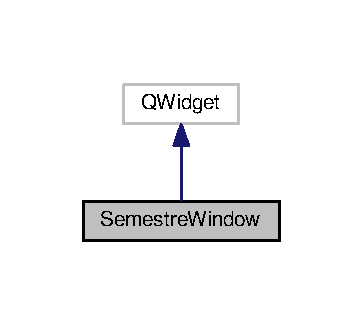
\includegraphics[width=174pt]{class_semestre_window__inherit__graph}
\end{center}
\end{figure}


Collaboration diagram for Semestre\-Window\-:
\nopagebreak
\begin{figure}[H]
\begin{center}
\leavevmode
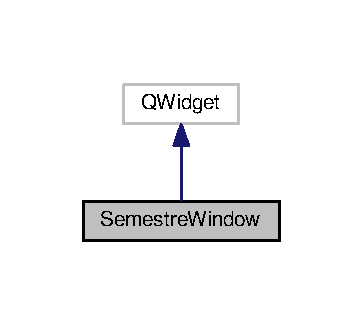
\includegraphics[width=174pt]{class_semestre_window__coll__graph}
\end{center}
\end{figure}
\subsection*{Public Slots}
\begin{DoxyCompactItemize}
\item 
void \hyperlink{class_semestre_window_aa7f626a4477fdd49811dcd55be412498}{ajouter} ()
\begin{DoxyCompactList}\small\item\em Ajout d'un semestre à un dossier existant. \end{DoxyCompactList}\end{DoxyCompactItemize}
\subsection*{Public Member Functions}
\begin{DoxyCompactItemize}
\item 
\hyperlink{class_semestre_window_a64a4a1613a3a1973f62334cd0688c2da}{Semestre\-Window} (const Q\-String \&l)
\begin{DoxyCompactList}\small\item\em Constructeur de \hyperlink{class_semestre_window}{Semestre\-Window}. \end{DoxyCompactList}\item 
Q\-String \hyperlink{class_semestre_window_a054c798f68ac93f5ec7e4d98d37faf28}{get\-Login} () const 
\begin{DoxyCompactList}\small\item\em Accès en lecture au login. \end{DoxyCompactList}\end{DoxyCompactItemize}


\subsection{Detailed Description}
Classe qui permet d'ajouter un semestre/une inscription à un uv, à un login existant. 

Definition at line 1128 of file U\-T\-Profiler.\-h.



\subsection{Constructor \& Destructor Documentation}
\hypertarget{class_semestre_window_a64a4a1613a3a1973f62334cd0688c2da}{\index{Semestre\-Window@{Semestre\-Window}!Semestre\-Window@{Semestre\-Window}}
\index{Semestre\-Window@{Semestre\-Window}!SemestreWindow@{Semestre\-Window}}
\subsubsection[{Semestre\-Window}]{\setlength{\rightskip}{0pt plus 5cm}Semestre\-Window\-::\-Semestre\-Window (
\begin{DoxyParamCaption}
\item[{const Q\-String \&}]{l}
\end{DoxyParamCaption}
)}}\label{class_semestre_window_a64a4a1613a3a1973f62334cd0688c2da}


Constructeur de \hyperlink{class_semestre_window}{Semestre\-Window}. 


\begin{DoxyParams}{Parameters}
{\em l} & \-: login du dossier auquel on veut ajouter une inscription à une uv \\
\hline
\end{DoxyParams}


Definition at line 734 of file Dossier\-Window.\-cpp.



\subsection{Member Function Documentation}
\hypertarget{class_semestre_window_aa7f626a4477fdd49811dcd55be412498}{\index{Semestre\-Window@{Semestre\-Window}!ajouter@{ajouter}}
\index{ajouter@{ajouter}!SemestreWindow@{Semestre\-Window}}
\subsubsection[{ajouter}]{\setlength{\rightskip}{0pt plus 5cm}void Semestre\-Window\-::ajouter (
\begin{DoxyParamCaption}
{}
\end{DoxyParamCaption}
)\hspace{0.3cm}{\ttfamily [slot]}}}\label{class_semestre_window_aa7f626a4477fdd49811dcd55be412498}


Ajout d'un semestre à un dossier existant. 

Fonction appelée lorsque l'utilisateur clique sur le bouton Ajouter de \hyperlink{class_semestre_window}{Semestre\-Window}.


\begin{DoxyParams}{Parameters}
{\em r} & \-: ligne de la cellule cliquée \\
\hline
{\em c} & \-: colonne de la cellule cliquée \\
\hline
\end{DoxyParams}


Definition at line 811 of file Dossier\-Window.\-cpp.

\hypertarget{class_semestre_window_a054c798f68ac93f5ec7e4d98d37faf28}{\index{Semestre\-Window@{Semestre\-Window}!get\-Login@{get\-Login}}
\index{get\-Login@{get\-Login}!SemestreWindow@{Semestre\-Window}}
\subsubsection[{get\-Login}]{\setlength{\rightskip}{0pt plus 5cm}Q\-String Semestre\-Window\-::get\-Login (
\begin{DoxyParamCaption}
{}
\end{DoxyParamCaption}
) const\hspace{0.3cm}{\ttfamily [inline]}}}\label{class_semestre_window_a054c798f68ac93f5ec7e4d98d37faf28}


Accès en lecture au login. 

\begin{DoxyReturn}{Returns}
l'attribut login 
\end{DoxyReturn}


Definition at line 1160 of file U\-T\-Profiler.\-h.



The documentation for this class was generated from the following files\-:\begin{DoxyCompactItemize}
\item 
\hyperlink{_u_t_profiler_8h}{U\-T\-Profiler.\-h}\item 
\hyperlink{_dossier_window_8cpp}{Dossier\-Window.\-cpp}\end{DoxyCompactItemize}

\hypertarget{class_u_t_profiler_exception}{\section{U\-T\-Profiler\-Exception Class Reference}
\label{class_u_t_profiler_exception}\index{U\-T\-Profiler\-Exception@{U\-T\-Profiler\-Exception}}
}


Classe permettant de gérer l'ensemble des exceptions de l'application.  




{\ttfamily \#include $<$U\-T\-Profiler.\-h$>$}

\subsection*{Public Member Functions}
\begin{DoxyCompactItemize}
\item 
\hyperlink{class_u_t_profiler_exception_aa8b3ca107d8de47ad4da8baa1e5a76d6}{U\-T\-Profiler\-Exception} (const Q\-String \&s)
\begin{DoxyCompactList}\small\item\em Constructeur Constructeur de la classe \hyperlink{class_u_t_profiler_exception}{U\-T\-Profiler\-Exception}, il crée une Q\-Msg\-Box avec le message passé en paramètre. \end{DoxyCompactList}\item 
\hypertarget{class_u_t_profiler_exception_ac43abbb72e3967b5c34f78838ae04de4}{\hyperlink{class_u_t_profiler_exception_ac43abbb72e3967b5c34f78838ae04de4}{$\sim$\-U\-T\-Profiler\-Exception} ()}\label{class_u_t_profiler_exception_ac43abbb72e3967b5c34f78838ae04de4}

\begin{DoxyCompactList}\small\item\em Destructeur Destructeur de la classe \hyperlink{class_u_t_profiler_exception}{U\-T\-Profiler\-Exception}. \end{DoxyCompactList}\end{DoxyCompactItemize}


\subsection{Detailed Description}
Classe permettant de gérer l'ensemble des exceptions de l'application. 

Cette classe reçoit un message en paramètre du constructeur, qu'elle affiche dans une Q\-Msg\-Box pour informer l'utilisateur quant à l'exception soulevée. 

Definition at line 88 of file U\-T\-Profiler.\-h.



\subsection{Constructor \& Destructor Documentation}
\hypertarget{class_u_t_profiler_exception_aa8b3ca107d8de47ad4da8baa1e5a76d6}{\index{U\-T\-Profiler\-Exception@{U\-T\-Profiler\-Exception}!U\-T\-Profiler\-Exception@{U\-T\-Profiler\-Exception}}
\index{U\-T\-Profiler\-Exception@{U\-T\-Profiler\-Exception}!UTProfilerException@{U\-T\-Profiler\-Exception}}
\subsubsection[{U\-T\-Profiler\-Exception}]{\setlength{\rightskip}{0pt plus 5cm}U\-T\-Profiler\-Exception\-::\-U\-T\-Profiler\-Exception (
\begin{DoxyParamCaption}
\item[{const Q\-String \&}]{s}
\end{DoxyParamCaption}
)}}\label{class_u_t_profiler_exception_aa8b3ca107d8de47ad4da8baa1e5a76d6}


Constructeur Constructeur de la classe \hyperlink{class_u_t_profiler_exception}{U\-T\-Profiler\-Exception}, il crée une Q\-Msg\-Box avec le message passé en paramètre. 


\begin{DoxyParams}{Parameters}
{\em s} & \-: Le message à afficher \\
\hline
\end{DoxyParams}


Definition at line 3 of file U\-T\-Profiler.\-cpp.



The documentation for this class was generated from the following files\-:\begin{DoxyCompactItemize}
\item 
\hyperlink{_u_t_profiler_8h}{U\-T\-Profiler.\-h}\item 
U\-T\-Profiler.\-cpp\end{DoxyCompactItemize}

\hypertarget{class_u_v}{\section{U\-V Class Reference}
\label{class_u_v}\index{U\-V@{U\-V}}
}


Classe permettant de décrire une des U\-Vs de l'U\-T\-C.  




{\ttfamily \#include $<$U\-T\-Profiler.\-h$>$}

\subsection*{Public Member Functions}
\begin{DoxyCompactItemize}
\item 
\hyperlink{class_u_v}{U\-V} \& \hyperlink{class_u_v_a47a46e1cf24e173b0b9694a4f404bb83}{operator=} (\hyperlink{class_u_v}{U\-V} \&other)
\begin{DoxyCompactList}\small\item\em Constructeur par recopie Permet de créer une nouvelle \hyperlink{class_u_v}{U\-V} qui soit la copie d'une \hyperlink{class_u_v}{U\-V} existante. \end{DoxyCompactList}\item 
\hyperlink{class_u_v_a4d98d82525d78e85c003c9acf2ee69bf}{U\-V} (const Q\-String \&c, const Q\-String \&t, const Q\-String \&r, unsigned int cs, unsigned int tm, unsigned int tsh, unsigned int sp, bool p, bool a)
\begin{DoxyCompactList}\small\item\em Constructeur Permet de créer une nouvelle \hyperlink{class_u_v}{U\-V}. \end{DoxyCompactList}\item 
\hypertarget{class_u_v_a898ad6c26e847fac8de1bd0cf4b88e92}{\hyperlink{class_u_v_a898ad6c26e847fac8de1bd0cf4b88e92}{U\-V} ()}\label{class_u_v_a898ad6c26e847fac8de1bd0cf4b88e92}

\begin{DoxyCompactList}\small\item\em Constructeur Vide Permet de créer un objet \hyperlink{class_u_v}{U\-V} non initialisé \end{DoxyCompactList}\item 
\hypertarget{class_u_v_a462f4f55409e6db802ed337a535678a7}{\hyperlink{class_u_v_a462f4f55409e6db802ed337a535678a7}{$\sim$\-U\-V} ()}\label{class_u_v_a462f4f55409e6db802ed337a535678a7}

\begin{DoxyCompactList}\small\item\em Destructeur. \end{DoxyCompactList}\item 
Q\-String \hyperlink{class_u_v_a4d5fe39505b3e474b41013dda0d2047a}{get\-Code} () const 
\begin{DoxyCompactList}\small\item\em Accesseur en lecture pour le code de l'\hyperlink{class_u_v}{U\-V}. \end{DoxyCompactList}\item 
Q\-String \hyperlink{class_u_v_afa7f5a8c7ea21bedcd00af1a1ff48221}{get\-Titre} () const 
\begin{DoxyCompactList}\small\item\em Accesseur en lecture pour la description de l'\hyperlink{class_u_v}{U\-V}. \end{DoxyCompactList}\item 
Q\-String \hyperlink{class_u_v_a845116e7deb10361c2723c9e90042a62}{get\-Responsable} () const 
\begin{DoxyCompactList}\small\item\em Accesseur en lecture pour le responsable de l'\hyperlink{class_u_v}{U\-V}. \end{DoxyCompactList}\item 
unsigned int \hyperlink{class_u_v_a348f309560bf41191f58fe47b6db9254}{get\-Credits\-C\-S} () const 
\begin{DoxyCompactList}\small\item\em Accesseur en lecture pour le nombre de crédits C\-S de l'\hyperlink{class_u_v}{U\-V}. \end{DoxyCompactList}\item 
unsigned int \hyperlink{class_u_v_af0ec1e2a228d470e0e9eac9bc7f7fc21}{get\-Credits\-T\-M} () const 
\begin{DoxyCompactList}\small\item\em Accesseur en lecture pour le nombre de crédits T\-M de l'\hyperlink{class_u_v}{U\-V}. \end{DoxyCompactList}\item 
unsigned int \hyperlink{class_u_v_aba3762bf14e1749bd721e736e366810a}{get\-Credits\-T\-S\-H} () const 
\begin{DoxyCompactList}\small\item\em Accesseur en lecture pour le nombre de crédits T\-S\-H de l'\hyperlink{class_u_v}{U\-V}. \end{DoxyCompactList}\item 
unsigned int \hyperlink{class_u_v_aed52076b1de90d10e053a21af0177888}{get\-Credits\-S\-P} () const 
\begin{DoxyCompactList}\small\item\em Accesseur en lecture pour le nombre de crédits S\-P de l'\hyperlink{class_u_v}{U\-V}. \end{DoxyCompactList}\item 
bool \hyperlink{class_u_v_ae2684b0333772600b1726d7179048290}{get\-Printemps} () const 
\begin{DoxyCompactList}\small\item\em Accesseur en lecture pour la disponibilité au printemps de l'\hyperlink{class_u_v}{U\-V}. \end{DoxyCompactList}\item 
bool \hyperlink{class_u_v_a242e4f2727fbf300c313a285cc4a402f}{get\-Automne} () const 
\begin{DoxyCompactList}\small\item\em Accesseur en lecture pour la disponibilité à l'automne de l'\hyperlink{class_u_v}{U\-V}. \end{DoxyCompactList}\item 
void \hyperlink{class_u_v_a53218978cc9e02e0cfd3f463608ff3bc}{set\-Code} (Q\-String $\ast$s)
\begin{DoxyCompactList}\small\item\em Accesseur en écriture pour le code de l'\hyperlink{class_u_v}{U\-V}. \end{DoxyCompactList}\item 
void \hyperlink{class_u_v_a3bf96f55fa44e5cb47ac6e77dc807dd3}{set\-Titre} (Q\-String $\ast$s)
\begin{DoxyCompactList}\small\item\em Accesseur en écriture de la description de l'\hyperlink{class_u_v}{U\-V}. \end{DoxyCompactList}\item 
void \hyperlink{class_u_v_a8827081089cc76e07f5adff29fdecc6f}{set\-Responsable} (Q\-String $\ast$s)
\begin{DoxyCompactList}\small\item\em Accesseur en écriture du nom du responsable de l'\hyperlink{class_u_v}{U\-V}. \end{DoxyCompactList}\item 
void \hyperlink{class_u_v_ae3368f076bd26424b3778fdb491595db}{set\-Credits\-C\-S} (unsigned int cs)
\begin{DoxyCompactList}\small\item\em Accesseur en écriture du nombre de crédits C\-S que permet de valider cette \hyperlink{class_u_v}{U\-V}. \end{DoxyCompactList}\item 
void \hyperlink{class_u_v_ab25119addbc4118a7e018f8b1e1b2bec}{set\-Credits\-T\-M} (unsigned int tm)
\begin{DoxyCompactList}\small\item\em Accesseur en écriture du nombre de crédits T\-M que permet de valider cette \hyperlink{class_u_v}{U\-V}. \end{DoxyCompactList}\item 
void \hyperlink{class_u_v_a0bb36d962f2d3138239fc361714c8a39}{set\-Credits\-T\-S\-H} (unsigned int tsh)
\begin{DoxyCompactList}\small\item\em Accesseur en écriture du nombre de crédits T\-S\-H que permet de valider cette \hyperlink{class_u_v}{U\-V}. \end{DoxyCompactList}\item 
void \hyperlink{class_u_v_a4e0cf1293aae9d67ecac693a1a5f427e}{setx\-Credits\-S\-P} (unsigned int sp)
\begin{DoxyCompactList}\small\item\em Accesseur en écriture du nombre de crédits S\-P que permet de valider cette \hyperlink{class_u_v}{U\-V}. \end{DoxyCompactList}\item 
void \hyperlink{class_u_v_a68343634c4849e078293a16d9bee6bcb}{set\-Printemps} (bool b)
\begin{DoxyCompactList}\small\item\em Accesseur en écriture de la disponibilité au printemps de cette \hyperlink{class_u_v}{U\-V}. \end{DoxyCompactList}\item 
void \hyperlink{class_u_v_a5b635154275bd3c5cd2cb4aa3465f115}{set\-Automne} (bool b)
\begin{DoxyCompactList}\small\item\em Accesseur en écriture de la disponibilité à l'automne de cette \hyperlink{class_u_v}{U\-V}. \end{DoxyCompactList}\item 
bool $\ast$ \hyperlink{class_u_v_ad7a90a92f1a93d7e32c93b59468484bb}{get\-Branche} ()
\begin{DoxyCompactList}\small\item\em Interroge la base de données et complète dynamiquement le tableau de booléens branches en fonction des formations dans laquelle cette \hyperlink{class_u_v}{U\-V} est diplomante. \end{DoxyCompactList}\item 
bool \hyperlink{class_u_v_a06ed5e33c1ac60b05c40ba6f575afde1}{operator!=} (\hyperlink{class_u_v}{U\-V} \&other)
\begin{DoxyCompactList}\small\item\em Teste l'égalité entre tous les champs de deux U\-Vs. \end{DoxyCompactList}\end{DoxyCompactItemize}


\subsection{Detailed Description}
Classe permettant de décrire une des U\-Vs de l'U\-T\-C. 

Cette classe permet de garder temporairement en mémoire l'ensemble des attributs d'une \hyperlink{class_u_v}{U\-V} et de les manipuler facilement. Cependant, un objet de cette classe n'est que temporaire, puisque toutes nos U\-Vs sont stockées dans notre Base de Données. 

Definition at line 110 of file U\-T\-Profiler.\-h.



\subsection{Constructor \& Destructor Documentation}
\hypertarget{class_u_v_a4d98d82525d78e85c003c9acf2ee69bf}{\index{U\-V@{U\-V}!U\-V@{U\-V}}
\index{U\-V@{U\-V}!UV@{U\-V}}
\subsubsection[{U\-V}]{\setlength{\rightskip}{0pt plus 5cm}U\-V\-::\-U\-V (
\begin{DoxyParamCaption}
\item[{const Q\-String \&}]{c, }
\item[{const Q\-String \&}]{t, }
\item[{const Q\-String \&}]{r, }
\item[{unsigned int}]{cs, }
\item[{unsigned int}]{tm, }
\item[{unsigned int}]{tsh, }
\item[{unsigned int}]{sp, }
\item[{bool}]{p, }
\item[{bool}]{a}
\end{DoxyParamCaption}
)\hspace{0.3cm}{\ttfamily [inline]}}}\label{class_u_v_a4d98d82525d78e85c003c9acf2ee69bf}


Constructeur Permet de créer une nouvelle \hyperlink{class_u_v}{U\-V}. 


\begin{DoxyParams}{Parameters}
{\em c} & \-: Code de la nouvelle \hyperlink{class_u_v}{U\-V} \\
\hline
{\em t} & \-: Description de la nouvelle \hyperlink{class_u_v}{U\-V} \\
\hline
{\em r} & \-: Nom du responsable de la nouvelle \hyperlink{class_u_v}{U\-V} \\
\hline
{\em cs} & \-: Nombre de crédits C\-S de la nouvelle \hyperlink{class_u_v}{U\-V} \\
\hline
{\em tm} & \-: Nombre de crédits T\-M de la nouvelle \hyperlink{class_u_v}{U\-V} \\
\hline
{\em tsh} & \-: Nombre de crédits T\-S\-H de la nouvelle \hyperlink{class_u_v}{U\-V} \\
\hline
{\em sp} & \-: Nombre de crédits S\-P de la nouvelle \hyperlink{class_u_v}{U\-V} \\
\hline
{\em p} & \-: Disponibilité au printemps de la nouvelle \hyperlink{class_u_v}{U\-V} \\
\hline
{\em a} & \-: Disponibilité à l'automne de la nouvelle \hyperlink{class_u_v}{U\-V} \\
\hline
\end{DoxyParams}


Definition at line 141 of file U\-T\-Profiler.\-h.



\subsection{Member Function Documentation}
\hypertarget{class_u_v_a242e4f2727fbf300c313a285cc4a402f}{\index{U\-V@{U\-V}!get\-Automne@{get\-Automne}}
\index{get\-Automne@{get\-Automne}!UV@{U\-V}}
\subsubsection[{get\-Automne}]{\setlength{\rightskip}{0pt plus 5cm}bool U\-V\-::get\-Automne (
\begin{DoxyParamCaption}
{}
\end{DoxyParamCaption}
) const\hspace{0.3cm}{\ttfamily [inline]}}}\label{class_u_v_a242e4f2727fbf300c313a285cc4a402f}


Accesseur en lecture pour la disponibilité à l'automne de l'\hyperlink{class_u_v}{U\-V}. 

\begin{DoxyReturn}{Returns}
True si l'\hyperlink{class_u_v}{U\-V} est disponible à l'automne, false sinon 
\end{DoxyReturn}


Definition at line 195 of file U\-T\-Profiler.\-h.

\hypertarget{class_u_v_ad7a90a92f1a93d7e32c93b59468484bb}{\index{U\-V@{U\-V}!get\-Branche@{get\-Branche}}
\index{get\-Branche@{get\-Branche}!UV@{U\-V}}
\subsubsection[{get\-Branche}]{\setlength{\rightskip}{0pt plus 5cm}bool $\ast$ U\-V\-::get\-Branche (
\begin{DoxyParamCaption}
{}
\end{DoxyParamCaption}
)}}\label{class_u_v_ad7a90a92f1a93d7e32c93b59468484bb}


Interroge la base de données et complète dynamiquement le tableau de booléens branches en fonction des formations dans laquelle cette \hyperlink{class_u_v}{U\-V} est diplomante. 

\begin{DoxyReturn}{Returns}
Le tableau de booléens complété dynamiquement. 
\end{DoxyReturn}


Definition at line 8 of file U\-T\-Profiler.\-cpp.

\hypertarget{class_u_v_a4d5fe39505b3e474b41013dda0d2047a}{\index{U\-V@{U\-V}!get\-Code@{get\-Code}}
\index{get\-Code@{get\-Code}!UV@{U\-V}}
\subsubsection[{get\-Code}]{\setlength{\rightskip}{0pt plus 5cm}Q\-String U\-V\-::get\-Code (
\begin{DoxyParamCaption}
{}
\end{DoxyParamCaption}
) const\hspace{0.3cm}{\ttfamily [inline]}}}\label{class_u_v_a4d5fe39505b3e474b41013dda0d2047a}


Accesseur en lecture pour le code de l'\hyperlink{class_u_v}{U\-V}. 

\begin{DoxyReturn}{Returns}
Le code de l'\hyperlink{class_u_v}{U\-V} 
\end{DoxyReturn}


Definition at line 155 of file U\-T\-Profiler.\-h.

\hypertarget{class_u_v_a348f309560bf41191f58fe47b6db9254}{\index{U\-V@{U\-V}!get\-Credits\-C\-S@{get\-Credits\-C\-S}}
\index{get\-Credits\-C\-S@{get\-Credits\-C\-S}!UV@{U\-V}}
\subsubsection[{get\-Credits\-C\-S}]{\setlength{\rightskip}{0pt plus 5cm}unsigned int U\-V\-::get\-Credits\-C\-S (
\begin{DoxyParamCaption}
{}
\end{DoxyParamCaption}
) const\hspace{0.3cm}{\ttfamily [inline]}}}\label{class_u_v_a348f309560bf41191f58fe47b6db9254}


Accesseur en lecture pour le nombre de crédits C\-S de l'\hyperlink{class_u_v}{U\-V}. 

\begin{DoxyReturn}{Returns}
Le nombre de credits C\-S que permet de valider cette \hyperlink{class_u_v}{U\-V} 
\end{DoxyReturn}


Definition at line 170 of file U\-T\-Profiler.\-h.

\hypertarget{class_u_v_aed52076b1de90d10e053a21af0177888}{\index{U\-V@{U\-V}!get\-Credits\-S\-P@{get\-Credits\-S\-P}}
\index{get\-Credits\-S\-P@{get\-Credits\-S\-P}!UV@{U\-V}}
\subsubsection[{get\-Credits\-S\-P}]{\setlength{\rightskip}{0pt plus 5cm}unsigned int U\-V\-::get\-Credits\-S\-P (
\begin{DoxyParamCaption}
{}
\end{DoxyParamCaption}
) const\hspace{0.3cm}{\ttfamily [inline]}}}\label{class_u_v_aed52076b1de90d10e053a21af0177888}


Accesseur en lecture pour le nombre de crédits S\-P de l'\hyperlink{class_u_v}{U\-V}. 

\begin{DoxyReturn}{Returns}
Le nombre de credits S\-P que permet de valider cette \hyperlink{class_u_v}{U\-V} 
\end{DoxyReturn}


Definition at line 185 of file U\-T\-Profiler.\-h.

\hypertarget{class_u_v_af0ec1e2a228d470e0e9eac9bc7f7fc21}{\index{U\-V@{U\-V}!get\-Credits\-T\-M@{get\-Credits\-T\-M}}
\index{get\-Credits\-T\-M@{get\-Credits\-T\-M}!UV@{U\-V}}
\subsubsection[{get\-Credits\-T\-M}]{\setlength{\rightskip}{0pt plus 5cm}unsigned int U\-V\-::get\-Credits\-T\-M (
\begin{DoxyParamCaption}
{}
\end{DoxyParamCaption}
) const\hspace{0.3cm}{\ttfamily [inline]}}}\label{class_u_v_af0ec1e2a228d470e0e9eac9bc7f7fc21}


Accesseur en lecture pour le nombre de crédits T\-M de l'\hyperlink{class_u_v}{U\-V}. 

\begin{DoxyReturn}{Returns}
Le nombre de credits T\-M que permet de valider cette \hyperlink{class_u_v}{U\-V} 
\end{DoxyReturn}


Definition at line 175 of file U\-T\-Profiler.\-h.

\hypertarget{class_u_v_aba3762bf14e1749bd721e736e366810a}{\index{U\-V@{U\-V}!get\-Credits\-T\-S\-H@{get\-Credits\-T\-S\-H}}
\index{get\-Credits\-T\-S\-H@{get\-Credits\-T\-S\-H}!UV@{U\-V}}
\subsubsection[{get\-Credits\-T\-S\-H}]{\setlength{\rightskip}{0pt plus 5cm}unsigned int U\-V\-::get\-Credits\-T\-S\-H (
\begin{DoxyParamCaption}
{}
\end{DoxyParamCaption}
) const\hspace{0.3cm}{\ttfamily [inline]}}}\label{class_u_v_aba3762bf14e1749bd721e736e366810a}


Accesseur en lecture pour le nombre de crédits T\-S\-H de l'\hyperlink{class_u_v}{U\-V}. 

\begin{DoxyReturn}{Returns}
Le nombre de credits T\-S\-H que permet de valider cette \hyperlink{class_u_v}{U\-V} 
\end{DoxyReturn}


Definition at line 180 of file U\-T\-Profiler.\-h.

\hypertarget{class_u_v_ae2684b0333772600b1726d7179048290}{\index{U\-V@{U\-V}!get\-Printemps@{get\-Printemps}}
\index{get\-Printemps@{get\-Printemps}!UV@{U\-V}}
\subsubsection[{get\-Printemps}]{\setlength{\rightskip}{0pt plus 5cm}bool U\-V\-::get\-Printemps (
\begin{DoxyParamCaption}
{}
\end{DoxyParamCaption}
) const\hspace{0.3cm}{\ttfamily [inline]}}}\label{class_u_v_ae2684b0333772600b1726d7179048290}


Accesseur en lecture pour la disponibilité au printemps de l'\hyperlink{class_u_v}{U\-V}. 

\begin{DoxyReturn}{Returns}
True si l'\hyperlink{class_u_v}{U\-V} est disponible au printemps, false sinon 
\end{DoxyReturn}


Definition at line 190 of file U\-T\-Profiler.\-h.

\hypertarget{class_u_v_a845116e7deb10361c2723c9e90042a62}{\index{U\-V@{U\-V}!get\-Responsable@{get\-Responsable}}
\index{get\-Responsable@{get\-Responsable}!UV@{U\-V}}
\subsubsection[{get\-Responsable}]{\setlength{\rightskip}{0pt plus 5cm}Q\-String U\-V\-::get\-Responsable (
\begin{DoxyParamCaption}
{}
\end{DoxyParamCaption}
) const\hspace{0.3cm}{\ttfamily [inline]}}}\label{class_u_v_a845116e7deb10361c2723c9e90042a62}


Accesseur en lecture pour le responsable de l'\hyperlink{class_u_v}{U\-V}. 

\begin{DoxyReturn}{Returns}
Le nom du responsable de l'\hyperlink{class_u_v}{U\-V} 
\end{DoxyReturn}


Definition at line 165 of file U\-T\-Profiler.\-h.

\hypertarget{class_u_v_afa7f5a8c7ea21bedcd00af1a1ff48221}{\index{U\-V@{U\-V}!get\-Titre@{get\-Titre}}
\index{get\-Titre@{get\-Titre}!UV@{U\-V}}
\subsubsection[{get\-Titre}]{\setlength{\rightskip}{0pt plus 5cm}Q\-String U\-V\-::get\-Titre (
\begin{DoxyParamCaption}
{}
\end{DoxyParamCaption}
) const\hspace{0.3cm}{\ttfamily [inline]}}}\label{class_u_v_afa7f5a8c7ea21bedcd00af1a1ff48221}


Accesseur en lecture pour la description de l'\hyperlink{class_u_v}{U\-V}. 

\begin{DoxyReturn}{Returns}
La description de l'\hyperlink{class_u_v}{U\-V} 
\end{DoxyReturn}


Definition at line 160 of file U\-T\-Profiler.\-h.

\hypertarget{class_u_v_a06ed5e33c1ac60b05c40ba6f575afde1}{\index{U\-V@{U\-V}!operator!=@{operator!=}}
\index{operator!=@{operator!=}!UV@{U\-V}}
\subsubsection[{operator!=}]{\setlength{\rightskip}{0pt plus 5cm}bool U\-V\-::operator!= (
\begin{DoxyParamCaption}
\item[{{\bf U\-V} \&}]{other}
\end{DoxyParamCaption}
)}}\label{class_u_v_a06ed5e33c1ac60b05c40ba6f575afde1}


Teste l'égalité entre tous les champs de deux U\-Vs. 


\begin{DoxyParams}{Parameters}
{\em other} & \-: l'autre \hyperlink{class_u_v}{U\-V} \\
\hline
\end{DoxyParams}
\begin{DoxyReturn}{Returns}
false si au moins un des deux champs diffère entre les deux U\-Vs, true sinon 
\end{DoxyReturn}


Definition at line 21 of file U\-T\-Profiler.\-cpp.

\hypertarget{class_u_v_a47a46e1cf24e173b0b9694a4f404bb83}{\index{U\-V@{U\-V}!operator=@{operator=}}
\index{operator=@{operator=}!UV@{U\-V}}
\subsubsection[{operator=}]{\setlength{\rightskip}{0pt plus 5cm}{\bf U\-V}\& U\-V\-::operator= (
\begin{DoxyParamCaption}
\item[{{\bf U\-V} \&}]{other}
\end{DoxyParamCaption}
)\hspace{0.3cm}{\ttfamily [inline]}}}\label{class_u_v_a47a46e1cf24e173b0b9694a4f404bb83}


Constructeur par recopie Permet de créer une nouvelle \hyperlink{class_u_v}{U\-V} qui soit la copie d'une \hyperlink{class_u_v}{U\-V} existante. 


\begin{DoxyParams}{Parameters}
{\em other} & \-: référence vers une \hyperlink{class_u_v}{U\-V} qui existe déjà \\
\hline
\end{DoxyParams}


Definition at line 127 of file U\-T\-Profiler.\-h.

\hypertarget{class_u_v_a5b635154275bd3c5cd2cb4aa3465f115}{\index{U\-V@{U\-V}!set\-Automne@{set\-Automne}}
\index{set\-Automne@{set\-Automne}!UV@{U\-V}}
\subsubsection[{set\-Automne}]{\setlength{\rightskip}{0pt plus 5cm}void U\-V\-::set\-Automne (
\begin{DoxyParamCaption}
\item[{bool}]{b}
\end{DoxyParamCaption}
)\hspace{0.3cm}{\ttfamily [inline]}}}\label{class_u_v_a5b635154275bd3c5cd2cb4aa3465f115}


Accesseur en écriture de la disponibilité à l'automne de cette \hyperlink{class_u_v}{U\-V}. 


\begin{DoxyParams}{Parameters}
{\em b} & \-: nouvelle disponibilité à l'automne de l'\hyperlink{class_u_v}{U\-V} \\
\hline
\end{DoxyParams}


Definition at line 240 of file U\-T\-Profiler.\-h.

\hypertarget{class_u_v_a53218978cc9e02e0cfd3f463608ff3bc}{\index{U\-V@{U\-V}!set\-Code@{set\-Code}}
\index{set\-Code@{set\-Code}!UV@{U\-V}}
\subsubsection[{set\-Code}]{\setlength{\rightskip}{0pt plus 5cm}void U\-V\-::set\-Code (
\begin{DoxyParamCaption}
\item[{Q\-String $\ast$}]{s}
\end{DoxyParamCaption}
)\hspace{0.3cm}{\ttfamily [inline]}}}\label{class_u_v_a53218978cc9e02e0cfd3f463608ff3bc}


Accesseur en écriture pour le code de l'\hyperlink{class_u_v}{U\-V}. 


\begin{DoxyParams}{Parameters}
{\em s} & \-: nouveau code de l'\hyperlink{class_u_v}{U\-V} \\
\hline
\end{DoxyParams}


Definition at line 200 of file U\-T\-Profiler.\-h.

\hypertarget{class_u_v_ae3368f076bd26424b3778fdb491595db}{\index{U\-V@{U\-V}!set\-Credits\-C\-S@{set\-Credits\-C\-S}}
\index{set\-Credits\-C\-S@{set\-Credits\-C\-S}!UV@{U\-V}}
\subsubsection[{set\-Credits\-C\-S}]{\setlength{\rightskip}{0pt plus 5cm}void U\-V\-::set\-Credits\-C\-S (
\begin{DoxyParamCaption}
\item[{unsigned int}]{cs}
\end{DoxyParamCaption}
)\hspace{0.3cm}{\ttfamily [inline]}}}\label{class_u_v_ae3368f076bd26424b3778fdb491595db}


Accesseur en écriture du nombre de crédits C\-S que permet de valider cette \hyperlink{class_u_v}{U\-V}. 


\begin{DoxyParams}{Parameters}
{\em cs} & \-: nouveau nombre de credits C\-S de l'\hyperlink{class_u_v}{U\-V} \\
\hline
\end{DoxyParams}


Definition at line 215 of file U\-T\-Profiler.\-h.

\hypertarget{class_u_v_ab25119addbc4118a7e018f8b1e1b2bec}{\index{U\-V@{U\-V}!set\-Credits\-T\-M@{set\-Credits\-T\-M}}
\index{set\-Credits\-T\-M@{set\-Credits\-T\-M}!UV@{U\-V}}
\subsubsection[{set\-Credits\-T\-M}]{\setlength{\rightskip}{0pt plus 5cm}void U\-V\-::set\-Credits\-T\-M (
\begin{DoxyParamCaption}
\item[{unsigned int}]{tm}
\end{DoxyParamCaption}
)\hspace{0.3cm}{\ttfamily [inline]}}}\label{class_u_v_ab25119addbc4118a7e018f8b1e1b2bec}


Accesseur en écriture du nombre de crédits T\-M que permet de valider cette \hyperlink{class_u_v}{U\-V}. 


\begin{DoxyParams}{Parameters}
{\em tm} & \-: nouveau nombre de credits T\-M de l'\hyperlink{class_u_v}{U\-V} \\
\hline
\end{DoxyParams}


Definition at line 220 of file U\-T\-Profiler.\-h.

\hypertarget{class_u_v_a0bb36d962f2d3138239fc361714c8a39}{\index{U\-V@{U\-V}!set\-Credits\-T\-S\-H@{set\-Credits\-T\-S\-H}}
\index{set\-Credits\-T\-S\-H@{set\-Credits\-T\-S\-H}!UV@{U\-V}}
\subsubsection[{set\-Credits\-T\-S\-H}]{\setlength{\rightskip}{0pt plus 5cm}void U\-V\-::set\-Credits\-T\-S\-H (
\begin{DoxyParamCaption}
\item[{unsigned int}]{tsh}
\end{DoxyParamCaption}
)\hspace{0.3cm}{\ttfamily [inline]}}}\label{class_u_v_a0bb36d962f2d3138239fc361714c8a39}


Accesseur en écriture du nombre de crédits T\-S\-H que permet de valider cette \hyperlink{class_u_v}{U\-V}. 


\begin{DoxyParams}{Parameters}
{\em tsh} & \-: nouveau nombre de credits T\-S\-H de l'\hyperlink{class_u_v}{U\-V} \\
\hline
\end{DoxyParams}


Definition at line 225 of file U\-T\-Profiler.\-h.

\hypertarget{class_u_v_a68343634c4849e078293a16d9bee6bcb}{\index{U\-V@{U\-V}!set\-Printemps@{set\-Printemps}}
\index{set\-Printemps@{set\-Printemps}!UV@{U\-V}}
\subsubsection[{set\-Printemps}]{\setlength{\rightskip}{0pt plus 5cm}void U\-V\-::set\-Printemps (
\begin{DoxyParamCaption}
\item[{bool}]{b}
\end{DoxyParamCaption}
)\hspace{0.3cm}{\ttfamily [inline]}}}\label{class_u_v_a68343634c4849e078293a16d9bee6bcb}


Accesseur en écriture de la disponibilité au printemps de cette \hyperlink{class_u_v}{U\-V}. 


\begin{DoxyParams}{Parameters}
{\em b} & \-: nouvelle disponibilité au printemps de l'\hyperlink{class_u_v}{U\-V} \\
\hline
\end{DoxyParams}


Definition at line 235 of file U\-T\-Profiler.\-h.

\hypertarget{class_u_v_a8827081089cc76e07f5adff29fdecc6f}{\index{U\-V@{U\-V}!set\-Responsable@{set\-Responsable}}
\index{set\-Responsable@{set\-Responsable}!UV@{U\-V}}
\subsubsection[{set\-Responsable}]{\setlength{\rightskip}{0pt plus 5cm}void U\-V\-::set\-Responsable (
\begin{DoxyParamCaption}
\item[{Q\-String $\ast$}]{s}
\end{DoxyParamCaption}
)\hspace{0.3cm}{\ttfamily [inline]}}}\label{class_u_v_a8827081089cc76e07f5adff29fdecc6f}


Accesseur en écriture du nom du responsable de l'\hyperlink{class_u_v}{U\-V}. 


\begin{DoxyParams}{Parameters}
{\em s} & \-: nouvau responsable de l'\hyperlink{class_u_v}{U\-V} \\
\hline
\end{DoxyParams}


Definition at line 210 of file U\-T\-Profiler.\-h.

\hypertarget{class_u_v_a3bf96f55fa44e5cb47ac6e77dc807dd3}{\index{U\-V@{U\-V}!set\-Titre@{set\-Titre}}
\index{set\-Titre@{set\-Titre}!UV@{U\-V}}
\subsubsection[{set\-Titre}]{\setlength{\rightskip}{0pt plus 5cm}void U\-V\-::set\-Titre (
\begin{DoxyParamCaption}
\item[{Q\-String $\ast$}]{s}
\end{DoxyParamCaption}
)\hspace{0.3cm}{\ttfamily [inline]}}}\label{class_u_v_a3bf96f55fa44e5cb47ac6e77dc807dd3}


Accesseur en écriture de la description de l'\hyperlink{class_u_v}{U\-V}. 


\begin{DoxyParams}{Parameters}
{\em s} & \-: nouvelle description de l'\hyperlink{class_u_v}{U\-V} \\
\hline
\end{DoxyParams}


Definition at line 205 of file U\-T\-Profiler.\-h.

\hypertarget{class_u_v_a4e0cf1293aae9d67ecac693a1a5f427e}{\index{U\-V@{U\-V}!setx\-Credits\-S\-P@{setx\-Credits\-S\-P}}
\index{setx\-Credits\-S\-P@{setx\-Credits\-S\-P}!UV@{U\-V}}
\subsubsection[{setx\-Credits\-S\-P}]{\setlength{\rightskip}{0pt plus 5cm}void U\-V\-::setx\-Credits\-S\-P (
\begin{DoxyParamCaption}
\item[{unsigned int}]{sp}
\end{DoxyParamCaption}
)\hspace{0.3cm}{\ttfamily [inline]}}}\label{class_u_v_a4e0cf1293aae9d67ecac693a1a5f427e}


Accesseur en écriture du nombre de crédits S\-P que permet de valider cette \hyperlink{class_u_v}{U\-V}. 


\begin{DoxyParams}{Parameters}
{\em sp} & \-: nouveau nombre de credits S\-P de l'\hyperlink{class_u_v}{U\-V} \\
\hline
\end{DoxyParams}


Definition at line 230 of file U\-T\-Profiler.\-h.



The documentation for this class was generated from the following files\-:\begin{DoxyCompactItemize}
\item 
\hyperlink{_u_t_profiler_8h}{U\-T\-Profiler.\-h}\item 
U\-T\-Profiler.\-cpp\end{DoxyCompactItemize}

\hypertarget{class_u_v_window}{\section{U\-V\-Window Class Reference}
\label{class_u_v_window}\index{U\-V\-Window@{U\-V\-Window}}
}


Inheritance diagram for U\-V\-Window\-:
\nopagebreak
\begin{figure}[H]
\begin{center}
\leavevmode
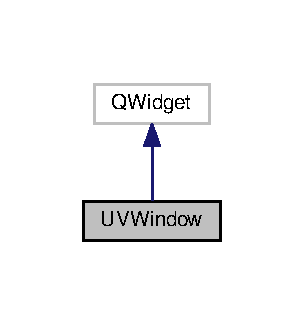
\includegraphics[width=146pt]{class_u_v_window__inherit__graph}
\end{center}
\end{figure}


Collaboration diagram for U\-V\-Window\-:
\nopagebreak
\begin{figure}[H]
\begin{center}
\leavevmode
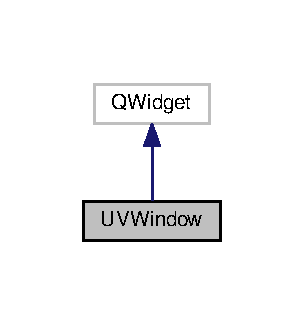
\includegraphics[width=146pt]{class_u_v_window__coll__graph}
\end{center}
\end{figure}
\subsection*{Public Slots}
\begin{DoxyCompactItemize}
\item 
\hypertarget{class_u_v_window_aa1af4be87f5aa569fa86606031033825}{void {\bfseries sauver} ()}\label{class_u_v_window_aa1af4be87f5aa569fa86606031033825}

\item 
\hypertarget{class_u_v_window_aeaf5064be5e25cc836722ed7cf6538e1}{void {\bfseries supprimer} ()}\label{class_u_v_window_aeaf5064be5e25cc836722ed7cf6538e1}

\item 
\hypertarget{class_u_v_window_a1fa3eada232c9db3a2cb81e32a6187aa}{void {\bfseries pbsauver\-Enable} ()}\label{class_u_v_window_a1fa3eada232c9db3a2cb81e32a6187aa}

\item 
\hypertarget{class_u_v_window_a225790ce1ed5e897b4f19e58c73b700f}{void {\bfseries rechercher} ()}\label{class_u_v_window_a225790ce1ed5e897b4f19e58c73b700f}

\item 
\hypertarget{class_u_v_window_a00cf849c430916afe95f6b727c5a900c}{void {\bfseries nouveau} ()}\label{class_u_v_window_a00cf849c430916afe95f6b727c5a900c}

\end{DoxyCompactItemize}
\subsection*{Public Member Functions}
\begin{DoxyCompactItemize}
\item 
\hypertarget{class_u_v_window_af473ab82c2310d5bf149bfa4ad795a5d}{void {\bfseries associer\-U\-V} (\hyperlink{class_u_v}{U\-V} $\ast$uv)}\label{class_u_v_window_af473ab82c2310d5bf149bfa4ad795a5d}

\item 
\hypertarget{class_u_v_window_a9ab0b242d5e666cb3bd5ce0aa0905e45}{void {\bfseries change\-T\-C} ()}\label{class_u_v_window_a9ab0b242d5e666cb3bd5ce0aa0905e45}

\item 
\hypertarget{class_u_v_window_a852bccb255fd5caf4ab26621435bcb0a}{void {\bfseries change\-H\-U\-T\-E\-C\-H} ()}\label{class_u_v_window_a852bccb255fd5caf4ab26621435bcb0a}

\item 
\hypertarget{class_u_v_window_ae91dde11f6ce5be07effc2e1f9f7b29e}{void {\bfseries change\-G\-B} ()}\label{class_u_v_window_ae91dde11f6ce5be07effc2e1f9f7b29e}

\item 
\hypertarget{class_u_v_window_a8bf1a182d841943322da78812dc802d5}{void {\bfseries change\-G\-I} ()}\label{class_u_v_window_a8bf1a182d841943322da78812dc802d5}

\item 
\hypertarget{class_u_v_window_a7eac2a6f7ae1b4e2c70b14be0c091b32}{void {\bfseries change\-G\-M} ()}\label{class_u_v_window_a7eac2a6f7ae1b4e2c70b14be0c091b32}

\item 
\hypertarget{class_u_v_window_ae6e564de6bd7b63e3a138f2a4a246466}{void {\bfseries change\-G\-P} ()}\label{class_u_v_window_ae6e564de6bd7b63e3a138f2a4a246466}

\item 
\hypertarget{class_u_v_window_a481ec8ffb35143328075ffd4612e5215}{void {\bfseries change\-G\-S\-M} ()}\label{class_u_v_window_a481ec8ffb35143328075ffd4612e5215}

\item 
\hypertarget{class_u_v_window_aedd3b862188eb04bf4caed25284eae4b}{void {\bfseries change\-G\-S\-U} ()}\label{class_u_v_window_aedd3b862188eb04bf4caed25284eae4b}

\end{DoxyCompactItemize}
\subsection*{Friends}
\begin{DoxyCompactItemize}
\item 
\hypertarget{class_u_v_window_a89f0e38a39f054c26a0ab852f8a79b18}{class {\bfseries Home\-Window}}\label{class_u_v_window_a89f0e38a39f054c26a0ab852f8a79b18}

\end{DoxyCompactItemize}


\subsection{Detailed Description}


Definition at line 937 of file U\-T\-Profiler.\-h.



The documentation for this class was generated from the following files\-:\begin{DoxyCompactItemize}
\item 
\hyperlink{_u_t_profiler_8h}{U\-T\-Profiler.\-h}\item 
U\-V\-Window.\-cpp\end{DoxyCompactItemize}

\chapter{File Documentation}
\hypertarget{_dossier_window_8cpp}{\section{Dossier\-Window.\-cpp File Reference}
\label{_dossier_window_8cpp}\index{Dossier\-Window.\-cpp@{Dossier\-Window.\-cpp}}
}


Fenêtre de gestion des dossiers.  


{\ttfamily \#include \char`\"{}U\-T\-Profiler.\-h\char`\"{}}\\*
Include dependency graph for Dossier\-Window.\-cpp\-:
\nopagebreak
\begin{figure}[H]
\begin{center}
\leavevmode
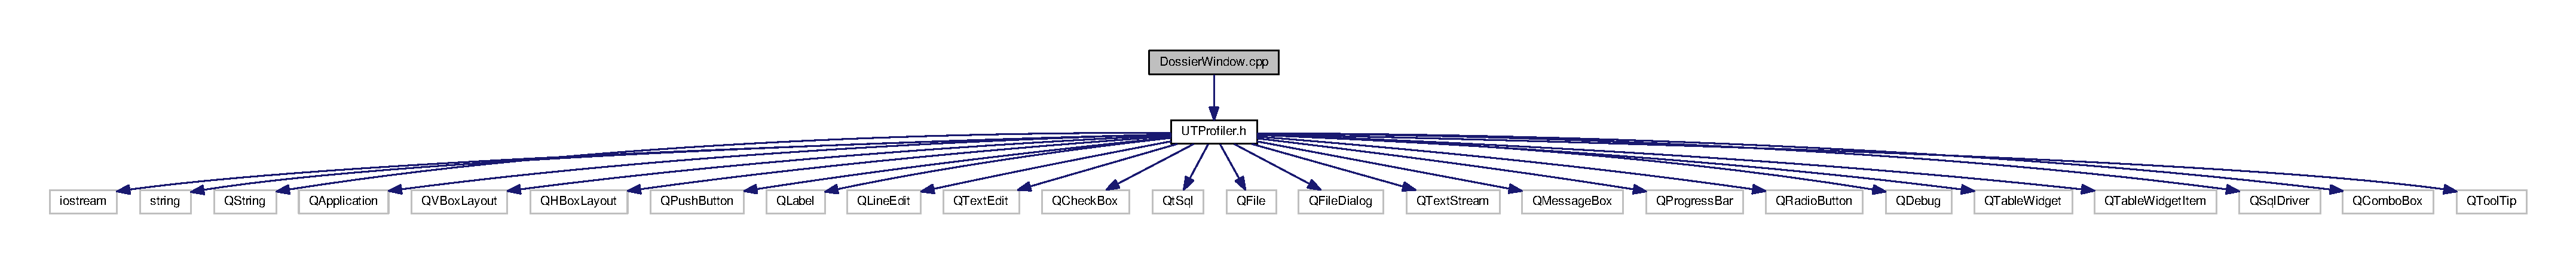
\includegraphics[width=350pt]{_dossier_window_8cpp__incl}
\end{center}
\end{figure}


\subsection{Detailed Description}
Fenêtre de gestion des dossiers. \begin{DoxyAuthor}{Author}
Gabrielle Rit et Timothée Monceaux 
\end{DoxyAuthor}


Definition in file \hyperlink{_dossier_window_8cpp_source}{Dossier\-Window.\-cpp}.


\hypertarget{_formation_window_8cpp}{\section{Formation\-Window.\-cpp File Reference}
\label{_formation_window_8cpp}\index{Formation\-Window.\-cpp@{Formation\-Window.\-cpp}}
}


Fenêtre de gestion des formations.  


{\ttfamily \#include \char`\"{}U\-T\-Profiler.\-h\char`\"{}}\\*
Include dependency graph for Formation\-Window.\-cpp\-:
\nopagebreak
\begin{figure}[H]
\begin{center}
\leavevmode
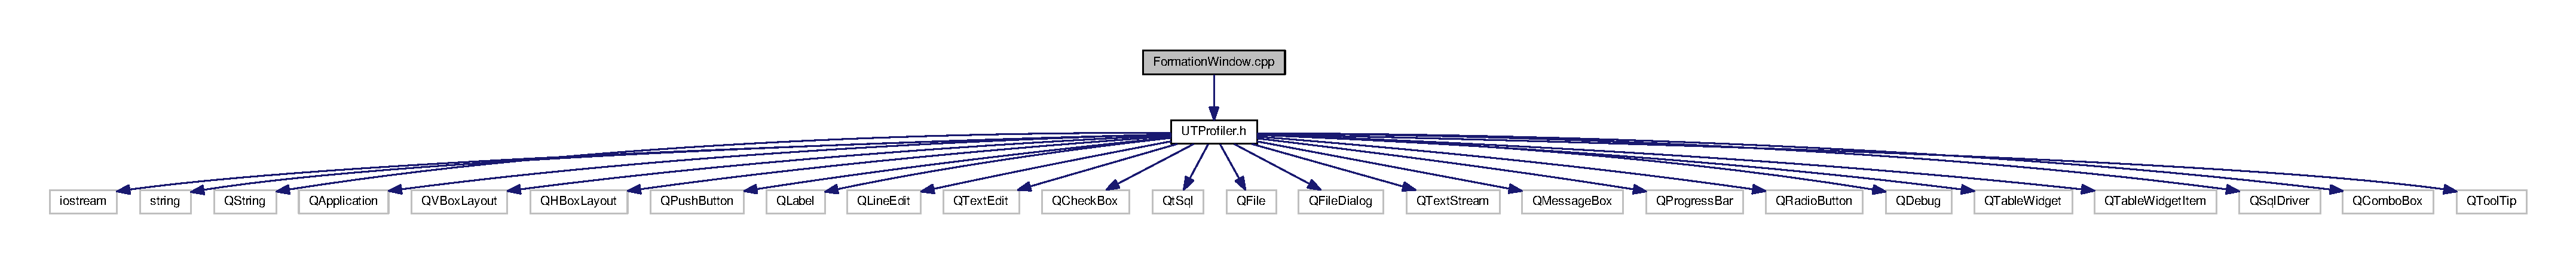
\includegraphics[width=350pt]{_formation_window_8cpp__incl}
\end{center}
\end{figure}


\subsection{Detailed Description}
Fenêtre de gestion des formations. \begin{DoxyAuthor}{Author}
Gabrielle Rit et Timothée Monceaux 
\end{DoxyAuthor}


Definition in file \hyperlink{_formation_window_8cpp_source}{Formation\-Window.\-cpp}.


\hypertarget{_home_window_8cpp}{\section{Home\-Window.\-cpp File Reference}
\label{_home_window_8cpp}\index{Home\-Window.\-cpp@{Home\-Window.\-cpp}}
}


Fenêtre d'accueil de U\-T\-Profiler.  


{\ttfamily \#include \char`\"{}U\-T\-Profiler.\-h\char`\"{}}\\*
Include dependency graph for Home\-Window.\-cpp\-:
\nopagebreak
\begin{figure}[H]
\begin{center}
\leavevmode
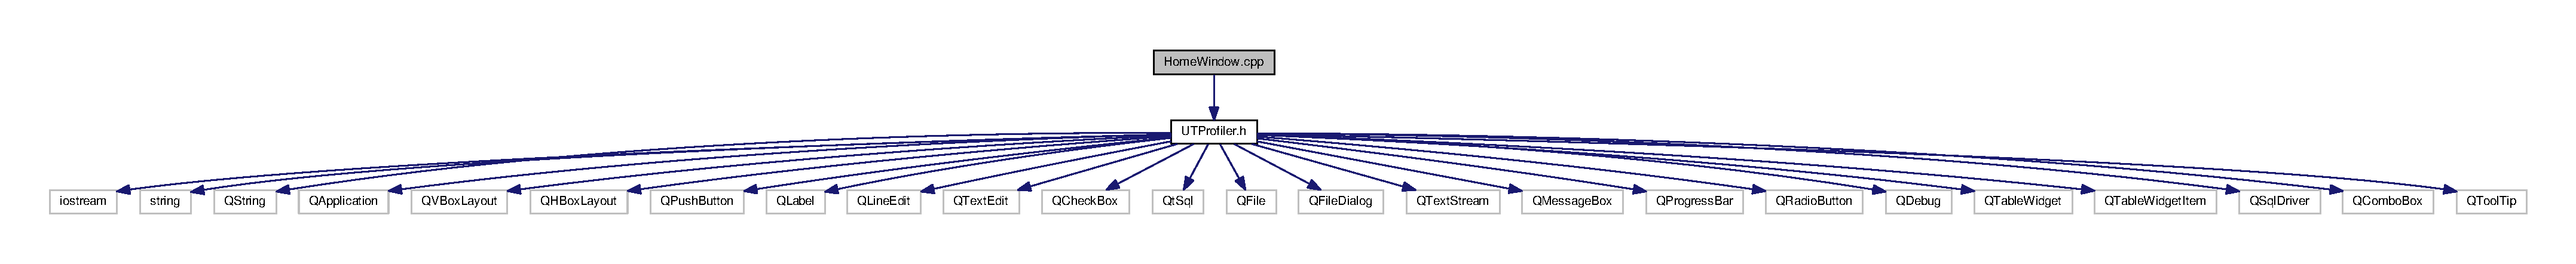
\includegraphics[width=350pt]{_home_window_8cpp__incl}
\end{center}
\end{figure}


\subsection{Detailed Description}
Fenêtre d'accueil de U\-T\-Profiler. \begin{DoxyAuthor}{Author}
Gabrielle Rit et Timothée Monceaux 
\end{DoxyAuthor}


Definition in file \hyperlink{_home_window_8cpp_source}{Home\-Window.\-cpp}.


\hypertarget{_interface_s_q_l_8cpp}{\section{Interface\-S\-Q\-L.\-cpp File Reference}
\label{_interface_s_q_l_8cpp}\index{Interface\-S\-Q\-L.\-cpp@{Interface\-S\-Q\-L.\-cpp}}
}


Fichier source où sont implémentées les méthodes de la classe \hyperlink{class_interface_s_q_l}{Interface\-S\-Q\-L}.  


{\ttfamily \#include \char`\"{}U\-T\-Profiler.\-h\char`\"{}}\\*
Include dependency graph for Interface\-S\-Q\-L.\-cpp\-:
\nopagebreak
\begin{figure}[H]
\begin{center}
\leavevmode
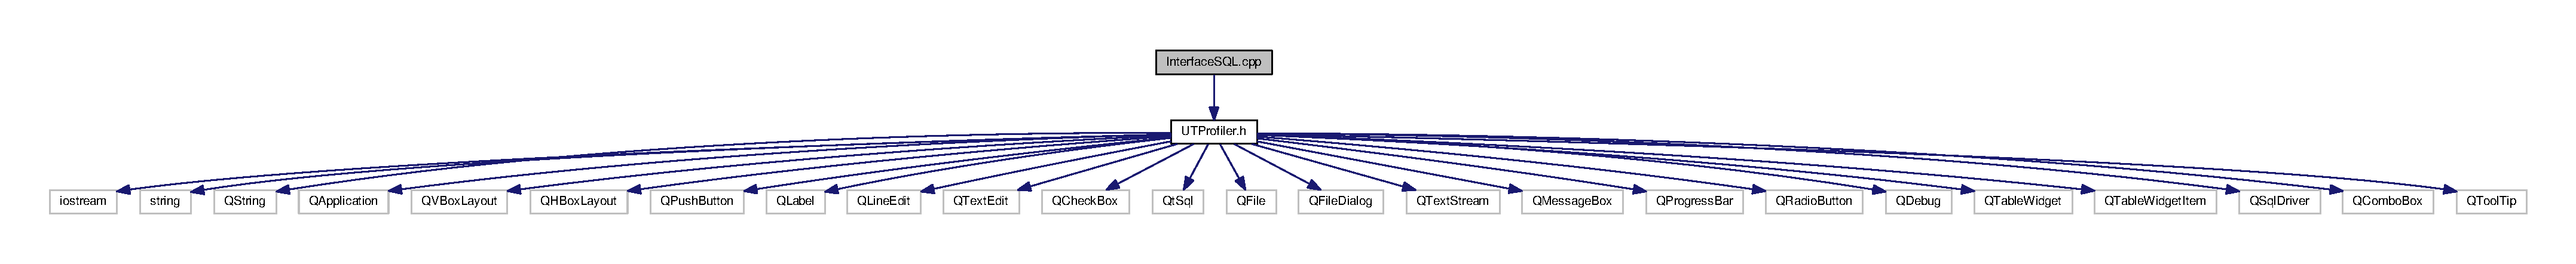
\includegraphics[width=350pt]{_interface_s_q_l_8cpp__incl}
\end{center}
\end{figure}


\subsection{Detailed Description}
Fichier source où sont implémentées les méthodes de la classe \hyperlink{class_interface_s_q_l}{Interface\-S\-Q\-L}. \begin{DoxyAuthor}{Author}
Gabrielle Rit Timothée Monceaux 
\end{DoxyAuthor}
\begin{DoxyVersion}{Version}
0.\-1 
\end{DoxyVersion}


Definition in file \hyperlink{_interface_s_q_l_8cpp_source}{Interface\-S\-Q\-L.\-cpp}.


\hypertarget{_u_t_profiler_8h}{\section{U\-T\-Profiler.\-h File Reference}
\label{_u_t_profiler_8h}\index{U\-T\-Profiler.\-h@{U\-T\-Profiler.\-h}}
}


Ce header recense les déclarations de toutes nos classes.  


{\ttfamily \#include $<$iostream$>$}\\*
{\ttfamily \#include $<$string$>$}\\*
{\ttfamily \#include $<$Q\-String$>$}\\*
{\ttfamily \#include $<$Q\-Application$>$}\\*
{\ttfamily \#include $<$Q\-V\-Box\-Layout$>$}\\*
{\ttfamily \#include $<$Q\-H\-Box\-Layout$>$}\\*
{\ttfamily \#include $<$Q\-Push\-Button$>$}\\*
{\ttfamily \#include $<$Q\-Label$>$}\\*
{\ttfamily \#include $<$Q\-Line\-Edit$>$}\\*
{\ttfamily \#include $<$Q\-Text\-Edit$>$}\\*
{\ttfamily \#include $<$Q\-Check\-Box$>$}\\*
{\ttfamily \#include $<$Qt\-Sql$>$}\\*
{\ttfamily \#include $<$Q\-File$>$}\\*
{\ttfamily \#include $<$Q\-File\-Dialog$>$}\\*
{\ttfamily \#include $<$Q\-Text\-Stream$>$}\\*
{\ttfamily \#include $<$Q\-Message\-Box$>$}\\*
{\ttfamily \#include $<$Q\-Progress\-Bar$>$}\\*
{\ttfamily \#include $<$Q\-Radio\-Button$>$}\\*
{\ttfamily \#include $<$Q\-Debug$>$}\\*
{\ttfamily \#include $<$Q\-Table\-Widget$>$}\\*
{\ttfamily \#include $<$Q\-Table\-Widget\-Item$>$}\\*
{\ttfamily \#include $<$Q\-Sql\-Driver$>$}\\*
{\ttfamily \#include $<$Q\-Combo\-Box$>$}\\*
{\ttfamily \#include $<$Q\-Tool\-Tip$>$}\\*
Include dependency graph for U\-T\-Profiler.\-h\-:
\nopagebreak
\begin{figure}[H]
\begin{center}
\leavevmode
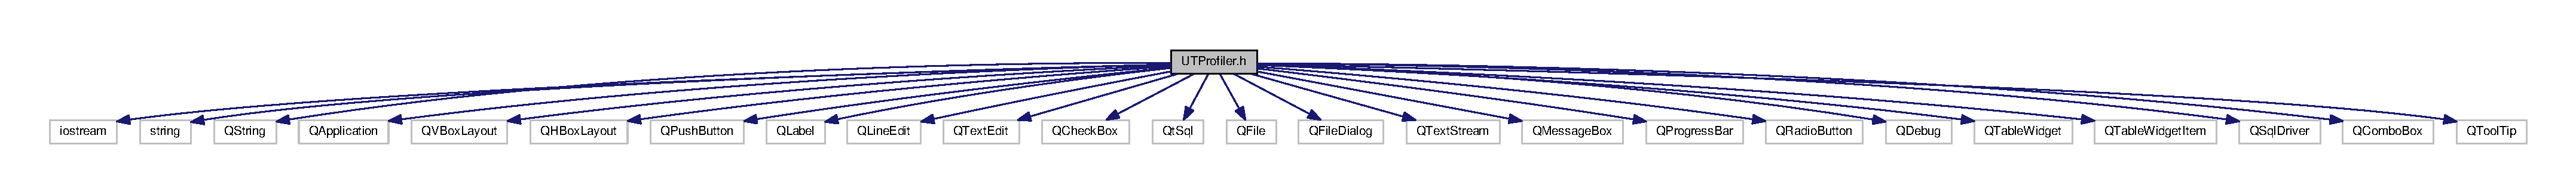
\includegraphics[width=350pt]{_u_t_profiler_8h__incl}
\end{center}
\end{figure}
\subsection*{Classes}
\begin{DoxyCompactItemize}
\item 
class \hyperlink{class_u_t_profiler_exception}{U\-T\-Profiler\-Exception}
\begin{DoxyCompactList}\small\item\em Classe permettant de gérer l'ensemble des exceptions de l'application. \end{DoxyCompactList}\item 
class \hyperlink{class_u_v}{U\-V}
\begin{DoxyCompactList}\small\item\em Classe permettant de décrire une des U\-Vs de l'U\-T\-C. \end{DoxyCompactList}\item 
class \hyperlink{class_inscription}{Inscription}
\begin{DoxyCompactList}\small\item\em Classe permettant de décrire l'inscription d'un étudiant à une \hyperlink{class_u_v}{U\-V} de l'U\-T\-C. \end{DoxyCompactList}\item 
class \hyperlink{class_formation_exterieure}{Formation\-Exterieure}
\begin{DoxyCompactList}\small\item\em Classe permettant de décrire une formation extérieure à l'U\-T\-C mais rapportant un certain nombre de crédits par équivalence. \end{DoxyCompactList}\item 
class \hyperlink{class_semestre}{Semestre}
\begin{DoxyCompactList}\small\item\em Classe permettant de décrire un semestre d'un étudiant de l'U\-T\-C. \end{DoxyCompactList}\item 
class \hyperlink{class_dossier}{Dossier}
\begin{DoxyCompactList}\small\item\em Classe représentant un dossier. \end{DoxyCompactList}\item 
class \hyperlink{class_formation}{Formation}
\begin{DoxyCompactList}\small\item\em Classe représentant une formation. \end{DoxyCompactList}\item 
class \hyperlink{class_interface_s_q_l}{Interface\-S\-Q\-L}
\begin{DoxyCompactList}\small\item\em Classe permettant la communication avec la base de données. \end{DoxyCompactList}\item 
class \hyperlink{class_new_u_v_window}{New\-U\-V\-Window}
\item 
class \hyperlink{class_u_v_window}{U\-V\-Window}
\item 
class \hyperlink{class_dossier_window}{Dossier\-Window}
\begin{DoxyCompactList}\small\item\em Classe pour la fenêtre qui permet de consulter, modifier, ajouter, supprimer un dossier. \end{DoxyCompactList}\item 
class \hyperlink{class_formation_ext_window}{Formation\-Ext\-Window}
\begin{DoxyCompactList}\small\item\em Classe qui permet d'ajouter une formation extérieure à un login existant. \end{DoxyCompactList}\item 
class \hyperlink{class_semestre_window}{Semestre\-Window}
\begin{DoxyCompactList}\small\item\em Classe qui permet d'ajouter un semestre/une inscription à un uv, à un login existant. \end{DoxyCompactList}\item 
class \hyperlink{class_new_formation_window}{New\-Formation\-Window}
\begin{DoxyCompactList}\small\item\em Classe qui permet d'ajouter une nouvelle formation. \end{DoxyCompactList}\item 
class \hyperlink{class_formation_window}{Formation\-Window}
\begin{DoxyCompactList}\small\item\em Classe de la fenêtre pour la gestion des formations. \end{DoxyCompactList}\item 
class \hyperlink{class_search_dossier_window}{Search\-Dossier\-Window}
\item 
class \hyperlink{class_retrouver_completion_window}{Retrouver\-Completion\-Window}
\item 
class \hyperlink{class_completion_profil_window}{Completion\-Profil\-Window}
\item 
class \hyperlink{class_home_window}{Home\-Window}
\begin{DoxyCompactList}\small\item\em Classe de la fenêtre d'accueil de U\-T\-Profiler. \end{DoxyCompactList}\item 
class \hyperlink{class_associer_u_v_window}{Associer\-U\-V\-Window}
\begin{DoxyCompactList}\small\item\em Classe de la fenêtre pour associer une uv à une formation. \end{DoxyCompactList}\item 
class \hyperlink{class_associer_filiere_window}{Associer\-Filiere\-Window}
\begin{DoxyCompactList}\small\item\em Classe de la fenêtre pour associer une filière à une branche. \end{DoxyCompactList}\end{DoxyCompactItemize}
\subsection*{Enumerations}
\begin{DoxyCompactItemize}
\item 
enum \hyperlink{_u_t_profiler_8h_a72fcaae0ef529616dd62b747e259d545}{Saison} \{ {\bfseries Printemps}, 
{\bfseries Automne}
 \}
\begin{DoxyCompactList}\small\item\em Recense les deux différents semestres d'une année à l'U\-T\-C \-: Printemps et Automne. \end{DoxyCompactList}\item 
enum \hyperlink{_u_t_profiler_8h_a89d667cddcff9ee818f60f3d9c6ac987}{Resultat} \{ \\*
{\bfseries A}, 
{\bfseries B}, 
{\bfseries C}, 
{\bfseries D}, 
\\*
{\bfseries E}, 
{\bfseries F\-X}, 
{\bfseries F}, 
{\bfseries R\-E\-S}, 
\\*
{\bfseries E\-C}
 \}
\begin{DoxyCompactList}\small\item\em Recense les différents statuts possibles quant à la validation d'une \hyperlink{class_u_v}{U\-V} \-: de A à F, En Cours, ou Réservé. \end{DoxyCompactList}\item 
enum \hyperlink{_u_t_profiler_8h_acd11e93d6654b761aee5afb6d2587ef7}{Categorie} \{ {\bfseries C\-S}, 
{\bfseries T\-M}, 
{\bfseries T\-S\-H}, 
{\bfseries S\-P}
 \}
\begin{DoxyCompactList}\small\item\em Recense les 4 Catégories d'\hyperlink{class_u_v}{U\-V} \-: C\-S, T\-M, T\-S\-H et S\-P. \end{DoxyCompactList}\end{DoxyCompactItemize}
\subsection*{Functions}
\begin{DoxyCompactItemize}
\item 
\hypertarget{_u_t_profiler_8h_a46cc93fa0ee0d1a8b574050903292776}{Q\-String {\bfseries check\-Syntax} (Q\-String s)}\label{_u_t_profiler_8h_a46cc93fa0ee0d1a8b574050903292776}

\item 
\hypertarget{_u_t_profiler_8h_a517805bc687ac358159e1c2bccde4cf5}{void {\bfseries Completion\-Profil} (\hyperlink{class_dossier}{Dossier} $\ast$dossier)}\label{_u_t_profiler_8h_a517805bc687ac358159e1c2bccde4cf5}

\end{DoxyCompactItemize}


\subsection{Detailed Description}
Ce header recense les déclarations de toutes nos classes. \begin{DoxyAuthor}{Author}
Gabrielle Rit Timothée Monceaux 
\end{DoxyAuthor}
\begin{DoxyVersion}{Version}
0.\-1 
\end{DoxyVersion}


Definition in file \hyperlink{_u_t_profiler_8h_source}{U\-T\-Profiler.\-h}.


%--- End generated contents ---

% Index
\newpage
\phantomsection
\addcontentsline{toc}{chapter}{Index}
\printindex

\end{document}
